%%% Årsrapportmal for nasjonale medisinske kvalitetsregistre.               %%%
%                                                                             %
% Suggested scheme for converitng to MS Word file:

% # compile latex source
% latex qRegAnnualReport.tex

% # make html from latex source
% htlatex qRegAnnualReport.tex

% # Next steps in libreoffice
% -open qRegAnnualReport.html
% -export as openoffice (odt)
% -open new odt-file
% -remove comments
% -set page size to A4
% -fix superscript on front page
% -remove footnote references that points to local html-file
% -adjust table
% -add page breaks
% -save as doc/docx
% -check that all is ok


% For print, bruk dokumentklassen 'book'. Bruk 'report' for å unngå blanke
% sider
\documentclass[norsk, a4paper, twocolumn]{report}

\usepackage[utf8x]{inputenc}
\usepackage[norsk]{babel}
\usepackage{longtable}
\usepackage{multicol}
%\usepackage{color}
\usepackage{wasysym}
\usepackage[raggedright]{titlesec}
\usepackage{color}
\usepackage{soul}
\usepackage{framed}

%Fra samledokument:
\usepackage{textcomp}
\usepackage{fancyhdr}
\pagestyle{fancy}
%\usepackage{amsmath}
\usepackage{rotating} %add rotating for plain tables
\usepackage{pdflscape} %add rotating/landcape for pdf
\usepackage[pdftex, colorlinks, linkcolor=OffBlaa3, urlcolor=OffBlaa3]{hyperref}
\usepackage{afterpage} 
%\afterpage{\clearpage} %unngå sideskift etter floatflsuh
%\restylefloat{figure} %gjør det mulig å angi H som parameter for plassering av floats
%for nice looking tabs
\usepackage{booktabs}


%bytte font
\renewcommand{\familydefault}{\sfdefault}

%setter grå skrift fremfort sort
\usepackage{xcolor}
\usepackage{graphicx}


% Gjør alle lenker mørkeblå
\definecolor{darkblue}{rgb}{0.0,0.0,0.3}
\hypersetup{colorlinks,breaklinks,linkcolor=darkblue,urlcolor=darkblue,anchorcolor=darkblue,citecolor=darkblue}

% Ikke sett inn sidenummer for ``Parts''
\makeatletter
\let\sv@endpart\@endpart
\def\@endpart{\thispagestyle{empty}\sv@endpart}
\makeatother

% Ikke bruk innrykk for nye avsnitt, men heller litt større vertikal avstand
\setlength{\parindent}{0pt}
\setlength{\parskip}{1ex plus 0.5ex minus 0.2ex}


% Sett registerets navn
\def \registernavn {\textit{Nasjonalt kvalitetsregister for ryggkirugi (NKR)}}


% tittelting
\title{\registernavn \\ \textbf{Årsrapport for 2016 med \\
plan for forbedringstiltak}}

\usepackage{authblk}
\author[1]{Tore Solberg}
\author[2]{Lena Ringstad Olsen}

\affil[1]{Universitetssykehuset Nord Norge (UNN)}
\affil[2]{SKDE}

\date{\parbox{\linewidth}{\centering%
  \today\endgraf\bigskip
  \begin{small}
  På vegne av fagrådet:\endgraf\medskip
  Øystein P Nygaard, St. Olav, HM (fagrådsleder)\\
  Jens Ivar Brox, OUS, HSØ\\
  Ivar Austevoll, HUS, HV\\
  Christian Hellum, OUS, HSØ\\
  Greger Lønne, NOP, HSØ\\
  Frode Kolstad, NNKF, HSØ\\
  Stein Andersen (Adm. leder, Ryggforeningen)\\
  Tore K Solberg, UNN, HN (faglig leder)\endgraf
  \end{small}
}}

\renewcommand*{\Authand}{, }
\renewcommand*{\Authands}{ og }
\renewcommand\Authfont{\scshape}
\renewcommand\Affilfont{\itshape\small}


% stil for veiledende tekst
\definecolor{guidegray}{rgb}{0.2,0.2,0.2}
\newcommand{\guide}[1] {
	\textit{[\textcolor{guidegray}{#1}]}
	}


% overstyre mulige ord-deling-er
\hyphenation{stadium-vurder-ing system-atiske pasi-ent-rap-porterte
retnings-linjer hjemmelsgrunnlag data-behandlings-ansvar nasjon-ale
indi-kator-er styrings-gruppe}

%% Preamble, klippet ut fra Resultatkapittelet


\begin{document}

\maketitle

\onecolumn


% Ta ut hele kapittelet ved bruk til faktisk rapport.
% Av en eller annen grunn ønskes også versjonsoversikten tatt ut fra malen\ldots
% Tas inn igjen ved å fjerne løkka rundt



\tableofcontents


\part{Årsrapport}\label{par:rap}
Analysene i denne rapporten er gjort på vegne av fagrådet til Nasjonalt
kvalitetsregister for ryggkirurgi i samarbeid med Senter for Klinisk Evaluering og
Dokumentasjon (SKDE), Helse Nord. Rapporten er i hovedsak hentet direkte fra
registerets rapportsystem som er tilgjengelig online for brukerne av registeret.
Rapportene oppdateres automatisk og kontinuerlig etter hvert som nye data
registreres. NKR’s rapportsystem inkludert samlerapporten er utviklet i samarbeid
med statistiker Lena Ringstad Olsen og Are Edvardsen (SKDE/Helse Nord) IKT).
 Dekningsgrad-analysene er gjennomført i et samarbeid mellom SKDE (statistiker Alexander Walnum), NPR og NKR. Forbruksrater for rygg og nakkekirurgi er bergnet i samarbeid med Bård Uleberg (SKDE).



\textbf{Det er viktig å merke seg at rapporten ikke evaluerer alternative behandlingformer til kirurgi. Sammenstilling av resultater er gjort uten justering for forskjeller i pasientpopulasjonene til de uklike sykehusene. Kvalitetsindikatorene er valgt ut fra at de kan peke på kvalitetsforskjeller. Om dette er tilfelle kan best vurderes av fagfolk ved de enkelte sykehus.Indikatorene kan dermed være et grunnlag for kvalitetsforbedring og  praksisendring.} 

\thispagestyle{empty}



\chapter{Sammendrag/Summary}


Nasjonalt Kvalitetsregister for Ryggkirurgi (NKR) har som mål å sikre og forbedre 
kvaliteten på rygg og nakkekirurgi som utføres ved norske sykehus.

For degenerativ rygg var tilslutningen på sykehusnivå 100 \% og dekningsgraden var 64,3 \% på individnivå i
2016. Tilsvarende tall for NKR degenerativ nakke var 100 og 75 \% i 2015. Dekningsgradsanalysene for nakkekirurgi blir ikke oppdatert før i årsrapporten for 2017. At
dekningsgraden er utilfredsstillende skyldes i første rekke mangelfulle rutiner for
rapportering av akutt, ikke planlagt kirurgi ved flere sykehus, spesielt i helger,
høytider og ferier. Dette er veldokumentert i dekningsgradsanalysen med tilhørende frafallsanalyser utført av Norsk Pasientregister (Helsedirektoratet).
Pasientgruppene opplever en sterk, klinisk relevant og statistisk signifikant
forbedring av smerterelatert funksjon i dagliglivets aktiviteter, livskvalitet og
inntekstgivendearbeidsevne etter operasjon.
 Det er stor praksisvariasjon hva angår liggetid på sykehus og bruk av mer omfattende kirurgi, slik som avstivninsoperasjoner (fusjonskirurgi) i behandling av spinal stenose. Både for nakke og ryggkirurgi er det forskjeller i behandlingsresultatet ved ulike sykehus. En
god del av variasjonen kan forklares av at pasientpopulasjonene er forskjellige og at
indikasjonsstillingen for kirurgi er ulik. Strengere indikasjonsstilling, færre reoperasjoner, reduserte
ventetider og bedre kommunikasjon med fremmedspråklige vil sannsynligvis kunne
bedre operasjonsresultatene.

\section*{Summary in English}

The Norwegian registry for spine surgery (NORspine) aims at improving the quality of surgical treatment for degenerative disorders in the cervical and lumbar spine. 
In 2016, the  national coverage of the NORspine was 100 \% at the institutional level and 64,3 \% at the individual level for lumbar spine surgery. For cervical spine surgery , the corresponding figures were 100 \%  and 75 \% in 2015 (will be updated with new figures form 2017 in 2018). The patients experienced strong and clinically relevant improvements of pain, disability and health-related quality of life after surgery. There was a large practice variation in the number of days patients are hospitalized and in the use of more comprehensive operations (fusions) in surgery for spinal stenosis.There is also variation in clinical results between hospitals, both for patients operated in the cervical and lumbar spine. Many of there differences can be explained by variation in patient populations and differences in indications (criteria) used for performing surgery. Stronger indications, less re-operations, faster access to surgery. better communication with patients who are foreign language users could improve results.



\chapter{Registerbeskrivelse}\label{cha:reg}


\section{Bakgrunn og formål}


\subsection{Bakgrunn for registeret}\label{sec:bak}
Registeret bygger videre på et regionalt register etablert ved UNN i 2000. Data fra det regionale registeret har blitt brukt til å validere måleinstrumenter og metoder som brukes i NKR. Utviklingsfasen for NKR startet for fullt etter 30. oktober 2006 ble det gitt konsesjon fra Datatilsynet slik at registeret kunne ekspanderes til et nasjonalt register (NKR), og samme år kom en registerplattform med kobling til Folkeregisteret på plass. I løpet av 2007 – 2010 har NKR etablert databehandleravtaler med samtlige HF og bistått de hvert sykehus med oppkobling via Norsk Helsenett. En alternativ VPN -løsning ble også utviklet i 2009 slik at sykehus utenfor Norsk Helsenett også fikk mulighet for oppkobling. I løpet av 2010 kunne derfor alle sykehus teknisk sett nå registerportalen til NKR.

Kostnadsfri online bestilling og distribusjon av spørreskjema/samtykkeerklæring fra trykkeriet er etablert for brukerne. Det har vært gjort et større arbeid knyttet til dokumentasjon (Registerbeskrivelse) og brukerveiledning (Brukermanual og hjelpefunksjon i databasen) og presentasjon av NKR på faglige møter i inn- og utland. En forbedret Versjon 2.0 av registeret ble satt i drift 1. september 2009 da NKR tok over all etterkontroll av pasienter 3 og 12 måneder etter operasjon, ved å sende ut og registrere skannbare spørreskjema uten å involvere de enkelte sykehusene. Dette medførte at pasientene selv begynte å rapporterte postoperative komplikasjoner, basert på definerte spørsmål i skjemaene. 

NKR fikk konsesjon for uttrekk av data fra NPR i 2010. I 2011 har NKR etablert en standardisert metode for å vaske og kvalitetssikre datauttrekk fra NPR som bygger på en kombinasjon av prosedyrekoder (NCSP) og diagnosekoder (ICD-10). Videre er det utarbeidet en standardisert metode for å beregne alder og kjønnsjusterte operasjonsrater som kan splittes på type inngrep (lett og tung ryggkirurgi), pasientens bosted (kommune, HF og RHF) og behandlingssted (kirurgisk enhet, HF, RHF og offentlig / privat virksomhet).

NKR har nå fått på plass en direkte kobling av data på individ nivå mellom NKR og NPR slik at dekningsgradsanalysene kan bli mer standardiserte og nøyaktige. Rapportsystemet til NKR gjennomgikk en betydelig forbedring ila 2011 og 2012. NKR tilbyr standardiserte og automatisk genererte samlerapporter i PDF format for de ulike HF som distribueres per e-post til sykehusene.  Nye og interaktive online rapporter og tilbud om nedlastning av egne rådata ble utviklet i 2013 og 2014. Et tilsvarende rapportsystem for NKR, degenerativ nakke ble etablert og satt i drift i 2016. NKR er nå i gang med å etablere en ny registerplattform for NKR (samme som degenerativ nakke; Open Qreg) i samarbeid med Helse Nord IKT,  under Norsk Helsenett. Samtidig etableres det med en ny versjon 3.0 av NKR. Dette medfører en omfattende revisjon av eksisterende registreringsskjema. I dette arbeidet deltar en pasientorganisasjonen «Ryggforeningen» ved Stein Andersen. I 2016 ble han medlem i NKRs fagråd. Det ble i 2016 også etablert teknisk løsning med SMS-varsling som påminnelse ved etterkontroll. Denne løsningen skal komme i drift i løpet av 2017.

\subsection{Registerets formål}\label{sec:for}
Nasjonalt Kvalitetsregister for Ryggkirurgi (NKR) har som mål å sikre og forbedre kvaliteten på ryggkirurgi som utføres ved norske sykehus. 
Målgruppen er pasienter som blir operert for degenerative tilstander i rygg og nakke (LS og C-kolumna) ved alle offentlige og private sykehus. Degenerative tilstander kan skape trange forhold for nervestrukturer og på grunn av skiveprolaps, benpåleiringer, fortykkelse av leddbånd/bindevev og feilstillinger i ryggsøylen. Pasientene har ofte sterke smerter, dårlig fysisk funksjon som medfører arbeidsuførhet og redusert livskvalitet.

Formålet med rapportene fra NKR er at det enkelte sykehus skal kunne holde oversikt over egne operasjonsresultater (ønskede og uønskede) og bruke informasjonen til forbedringsarbeid. Resultatene fra ”de beste sykehusene” og et nasjonalt gjennomsnitt brukes som referanseverdier for det enkelte sykehus.

NKR har bred støtte i fagmiljøet, både gjennom Norsk Spinalkirurgisk Forening, Norsk Nevrokirurgisk Forening, Norsk Ortopedisk Forening og andre fagmiljøer. I tillegg samarbeider NKR med pasientorganisasjonen "Ryggforeningen", som også er representert i fagrådet.  NKR ønsker å bidra til en bedre og mer oversiktlig helsetjeneste for pasientene. 

\section{Juridisk hjemmelsgrunnlag}\label{cha:jur}
Behandling av personopplysninger i NKR drives i henhold til konsesjonen fra Datatilsynet og bestemmelsene i helseregisterloven.  Registeret henter inn aktivt samtykke fra pasientene i henhold til konsesjonen.
NKR er i dag etablert som et elektronisk register hvor opplysningene legges fortløpende inn gjennom registerportalen www.helseregister.no via Norsk Helsenett. All pålogging til registeret skjer i dag med en to-faktorautentisering av brukerne. 



\section{Faglig ledelse og databehandlingsansvar}\label{cha:led}
Databehandlingsansvaret for NKR ble i 2011 flyttet fra administrerende direktør ved Helse Nord RHF til administrerende direktør ved Universitetssykehuset i Nord-Norge HF (UNN HF). Driften av registeret er finansiert av Helse Nord RHF og UNN HF. Sekretariatsfunksjoner og daglig ledelse er lokalisert til UNN HF.

Av hensyn til interessekonflikter er registeret faglig uavhengig og kan ikke motta støtte fra industrien eller andre med kommersielle interesser. Fagrådet til NKR har det faglige ansvaret og forvalter de data som samles inn og godkjenner eventuelle forskningsprosjekter knyttet til aggregerte, nasjonale data. Fagrådet skal i første rekke vurdere om prosjektene er i samsvar med formålet til NKR. Fagrådet er et kliniker og forskernettverk som består av representanter fra alle RHF-ene, en representant fra hhv. Norsk Ortopedisk og Nevrokirurgisk forening samt en brukerrepresentant fra pasientorganisasjonen ``Ryggforeningen''.

Registrerende avdeling er ansvarlig overfor fagrådet til NKR for feil i resultater på bakgrunn av feilregistreringer. Fagrådet til NKR, eller den de delegerer ansvaret til ved utlevering av data, er ansvarlig for vurderinger og tolkninger av aggregerte data fra de ulike sykehus. Kirurgiske enheter som NKR har databehandleravtaler med kan få utlevert egne data til kvalitetssikring og til forskning. For alle forskningsprosjekt forutsetter NKR at mottaker av data innhenter nødvendige godkjenninger fra offentlige instanser (for eksempel fra Personvernombud eller Regional etisk komité). Rapportsystemet (inkludert Årsrapporten) til NKR presenterer data på aggregert nivå og viser derfor ingen data om enkeltpersoner. I tilfeller der utvalget inneholder få registreringer og er kombinert med for eksempel demografisk informasjon, kan det ikke utelukkes at opplysningene kan tilbakeføres til enkeltpersoner. Det er NKR og fagrådet sitt ansvar å vurdere hvorvidt rapporter skal klassifiseres som sensitive eller ikke. 

%\subsection{Aktivitet i \\fagråd/referansegruppe}
\subsection{Aktivitet i fagråd/referansegruppe}
15. april 2016 ble det årlige brukermøtet og ett av tre fagrådsmøter avhold i Trondheim. På brukermøtet deltok representanter fra 25 forskjellige sykehusavdelinger. Dagen før ble fagrådsmøtet avholdt. Fagrådet har i tillegg avhold flere telefonmøter for gjennomgang av versjon 3.0 av degenerativ rygg, evaluering av søknader på forskningsprosjekt knyttet til NKR. I alt 3 av 4 nye forskningsprosjekt fra ulike kliniske/universitetsmiljø i Norge ble godkjent.





\chapter{Resultater}\label{cha:res}


\documentclass [norsk,a4paper,twoside]{article}\usepackage[]{graphicx}\usepackage[]{color}
%% maxwidth is the original width if it is less than linewidth
%% otherwise use linewidth (to make sure the graphics do not exceed the margin)
\makeatletter
\def\maxwidth{ %
  \ifdim\Gin@nat@width>\linewidth
    \linewidth
  \else
    \Gin@nat@width
  \fi
}
\makeatother

\definecolor{fgcolor}{rgb}{0.345, 0.345, 0.345}
\newcommand{\hlnum}[1]{\textcolor[rgb]{0.686,0.059,0.569}{#1}}%
\newcommand{\hlstr}[1]{\textcolor[rgb]{0.192,0.494,0.8}{#1}}%
\newcommand{\hlcom}[1]{\textcolor[rgb]{0.678,0.584,0.686}{\textit{#1}}}%
\newcommand{\hlopt}[1]{\textcolor[rgb]{0,0,0}{#1}}%
\newcommand{\hlstd}[1]{\textcolor[rgb]{0.345,0.345,0.345}{#1}}%
\newcommand{\hlkwa}[1]{\textcolor[rgb]{0.161,0.373,0.58}{\textbf{#1}}}%
\newcommand{\hlkwb}[1]{\textcolor[rgb]{0.69,0.353,0.396}{#1}}%
\newcommand{\hlkwc}[1]{\textcolor[rgb]{0.333,0.667,0.333}{#1}}%
\newcommand{\hlkwd}[1]{\textcolor[rgb]{0.737,0.353,0.396}{\textbf{#1}}}%
\let\hlipl\hlkwb

\usepackage{framed}
\makeatletter
\newenvironment{kframe}{%
 \def\at@end@of@kframe{}%
 \ifinner\ifhmode%
  \def\at@end@of@kframe{\end{minipage}}%
  \begin{minipage}{\columnwidth}%
 \fi\fi%
 \def\FrameCommand##1{\hskip\@totalleftmargin \hskip-\fboxsep
 \colorbox{shadecolor}{##1}\hskip-\fboxsep
     % There is no \\@totalrightmargin, so:
     \hskip-\linewidth \hskip-\@totalleftmargin \hskip\columnwidth}%
 \MakeFramed {\advance\hsize-\width
   \@totalleftmargin\z@ \linewidth\hsize
   \@setminipage}}%
 {\par\unskip\endMakeFramed%
 \at@end@of@kframe}
\makeatother

\definecolor{shadecolor}{rgb}{.97, .97, .97}
\definecolor{messagecolor}{rgb}{0, 0, 0}
\definecolor{warningcolor}{rgb}{1, 0, 1}
\definecolor{errorcolor}{rgb}{1, 0, 0}
\newenvironment{knitrout}{}{} % an empty environment to be redefined in TeX

\usepackage{alltt}
\addtolength{\hoffset}{-0.5cm}
\addtolength{\textwidth}{1cm}
\addtolength{\voffset}{-1cm}
\addtolength{\textheight}{2cm}


%for nice looking tabs
\usepackage{booktabs}

\usepackage[norsk]{babel}
\usepackage[utf8x]{inputenc}
\usepackage{textcomp}
\usepackage{fancyhdr}
\pagestyle{fancy}
\usepackage{amsmath}
\usepackage{rotating} %add rotating for plain tables
\usepackage{pdflscape} %add rotating/landcape for pdf

%bytte font
\renewcommand{\familydefault}{\sfdefault}

%setter grå skrift fremfort sort
\usepackage{xcolor}
\usepackage{graphicx}
\usepackage[pdftex, colorlinks, linkcolor=OffBlaa3, urlcolor=OffBlaa3]{hyperref}
\newcommand{\kommentar}[1]{\cbstart\textcolor{red}{#1\cbend}}
\IfFileExists{upquote.sty}{\usepackage{upquote}}{}
\begin{document}





\begin{knitrout}
\definecolor{shadecolor}{rgb}{0.969, 0.969, 0.969}\color{fgcolor}\begin{kframe}


{\ttfamily\noindent\itshape\color{messagecolor}{\#\# The following objects are masked \_by\_ .GlobalEnv:\\\#\# \\\#\#\ \ \ \  ASA, HovedInngrep, UforetrygdPre}}\end{kframe}
\end{knitrout}





\section{Forbruksrater av rygg- og nakkekirurgi i Norge (kilde: NPR/SSB)}
Variasjon i forbruksrater av rygg og nakkekirurgi mellom regioner kan 
gjenspeile ulik tilgjengelighet til helsetjenesten, men også praksisvariasjon som kan
representere i kvalitetsforskjeller i behandlingstilbudet. Figur \ref{fig:AA_Ryggkirurgi_BoRHF1}, \ref{fig:AA_Ryggkirurgi_BoHF1}, \ref{fig:AA_Nakkekirurgi_BoRHF1} og \ref{fig:AA_Nakkekirurgi_BoHF1} viser at det
er forskjeller i forbruksrater mellom ulike boområder i Norge i aldersgruppen 20 - 85 år. Disse kan ikke
forklares ut fra forskjeller i sykelighet. Tilgjengeligheten av rygg og nakkekirurgi er spesielt lav i boområdene til
Helse Nord, mens Helse Vest har gjennomgående høyest operasjonsrate. Forskjellene er størst for nakkekirurgi, der operasjonsraten er speiselt lav i Norland og 2-3 ganger høyere i boområdene til Stavanger og Østfold HF.
For degenerativ rygg har operasjonsraten hatt en svak økning (2\%) i Norge fra 156 i 2013  til 159 per 100000 innbygger per år i 2017. For nakkekirurgi har raten økt fra med 25\%, fra 24 til 30 per inbygger per 100.000 år i samme tidsperiode, og økningen har vært størst i Helse Vest RHF, \ref{fig:Rygkirurgi_line1.pdf} og \ref{fig:Nakkekirurgi_line1.pdf}.
 
\begin{figure}[ht]
\scalebox{0.9}{\includegraphics{Figurer/AA_Ryggkirurgi_BoRHF1.pdf}}
\caption{Kjønns- og aldersstandardiserte rater pr. 100 000 innbyggere, ryggkirurgi i RHf’enes opptaksområder, 2012-2017. Gjennomsnitt i perioden (søyler) og enkeltår (punkter).}
\label{fig:AA_Ryggkirurgi_BoRHF1}
\end{figure}

\begin{figure}[ht]
\scalebox{0.9}{\includegraphics{Figurer/AA_Ryggkirurgi_BoHF1.pdf}}
\caption{Kjønns- og aldersstandardiserte rater pr. 100 000 innbyggere, ryggkirurgi i helseforetakenes opptaksområder, 2012-2017. Gjennomsnitt i perioden (søyler) og enkeltår (punkter).}
\label{fig:AA_Ryggkirurgi_BoHF1}
\end{figure}


\begin{figure}[ht]
\scalebox{0.9}{\includegraphics{Figurer/AA_Nakkekirurgi_BoRHF1.pdf}}
\caption{Kjønns- og aldersstandardiserte rater pr. 100 000 innbyggere, nakkekirurgi i RHf’enes opptaksområder, 2012-2017. Gjennomsnitt i perioden (søyler) og enkeltår (punkter).}
\label{fig:AA_Nakkekirurgi_BoRHF1}
\end{figure}

\begin{figure}[ht]
\scalebox{0.9}{\includegraphics{Figurer/AA_Nakkekirurgi_BoHF1.pdf}}
\caption{Kjønns- og aldersstandardiserte rater pr. 100 000 innbyggere, nakkekirurgi i Hf’enes opptaksområder, 2012-2017. Gjennomsnitt i perioden (søyler) og enkeltår (punkter).}
\label{fig:AA_Nakkekirurgi_BoHF1}
\end{figure}

\begin{figure}[ht]
\scalebox{0.9}{\includegraphics{Figurer/Rygkirurgi_line1.pdf}}
\caption{Kjønns- og aldersstandardiserte rater pr. 100 000 innbyggere, ryggkirurgi i RHf’enes opptaksområder, 2013-2017 per år (punkter).}
\label{fig:Rygkirurgi_line1}
\end{figure}

\begin{figure}[ht]
\scalebox{0.9}{\includegraphics{Figurer/Nakkekirurgi_line1.pdf}}
\caption{Kjønns- og aldersstandardiserte rater pr. 100 000 innbyggere, nakkekirurgi i RHf’enes opptaksområder, 2013-2017 per år (punkter).}
\label{fig:Nakkekirurgi_line1}
\end{figure}




\clearpage



\section{Oppsummeringstall for NKR}




\subsection{Degenerativ nakke}

% latex table generated in R 3.5.0 by xtable 1.8-2 package
% Wed Sep 26 12:16:31 2018
\begin{table}[ht]
\centering
\begin{tabular}{lrrrrrr}
  \hline
 & 2013 & 2014 & 2015 & 2016 & 2017 & Sum \\ 
  \hline
Aleris Helse AS & 0 & 0 & 0 & 5 & 17 & 22 \\ 
  Haukeland USH & 94 & 139 & 118 & 98 & 111 & 637 \\ 
  Oslo, RH & 222 & 303 & 307 & 281 & 318 & 1628 \\ 
  Oslo, Ullevål USH & 83 & 88 & 148 & 113 & 182 & 659 \\ 
  Oslofjordklin., øst & 102 & 195 & 173 & 180 & 178 & 828 \\ 
  Oslofjordklinikken Vest & 0 & 13 & 47 & 50 & 50 & 160 \\ 
  Stavanger USH & 119 & 145 & 186 & 146 & 164 & 867 \\ 
  Tromsø, UNN & 47 & 70 & 49 & 57 & 61 & 331 \\ 
  Trondheim, St. Olav & 104 & 123 & 114 & 123 & 119 & 671 \\ 
  Volvat & 0 & 0 & 2 & 5 & 0 & 7 \\ 
  Sum & 771 & 1076 & 1144 & 1058 & 1200 & 5810 \\ 
   \hline
\end{tabular}
\caption{Antall registreringer av nakkeoperasjoner ved hver avdeling siste 5 år, samt totalt siden 2012.} 
\label{tab:AntRegNakke}
\end{table}



Tabell \ref{tab:AntRegNakke} viser antall 
registreringer gjort ved de respektive avdelinger siste 5 år. Registreringene startet i 2012. 
Det er  
10 avdelinger som rapporterer til NKR degenerativ nakke. Totalt er det registrert 5810 operasjoner siden oppstart (2012). Av disse er 54.9\% utført på menn og 45.1\% på kvinner.
Siste inngrep registrert i datauttrekket som ligger til grunn for denne rapporten, ble utført 
2017-12-27. 
\par




\subsection{Degenerativ rygg}

Tabell \ref{tab:AntReg} viser antall 
registreringer gjort ved de respektive avdelinger siste 5 år. Det er  
47 avdelinger som har registrerer i perioden 2011 til 2017. Totalt er det registrert 30108 
operasjoner. Av disse er 52.7\% utført på menn og 47.3\% på kvinner.
Siste rygginngrep registrert i datauttrekket som ligger til grunn for denne rapporten, ble utført 
2017-12-30. Siden oppstart i 2007 til og med 2017 er det totalt registrert 38612 operasjoner i NKR degenerativ rygg. 
\par

Flere enheter har hatt en stor og gledelig økning av antall registreringer til NKR, degenerativ rygg. Spesielt gjelder dette Kristiansund, Larvik, Førde og Ullevål (nevrokirurgisk avd.).
% latex table generated in R 3.5.0 by xtable 1.8-2 package
% Wed Sep 26 12:16:31 2018
\begin{table}[ht]
\centering
\begin{tabular}{lrrrrrr}
  \hline
 & 2013 & 2014 & 2015 & 2016 & 2017 & Sum \\ 
  \hline
Ahus & 151 & 67 & 137 & 186 & 226 & 824 \\ 
  Aleris, Bergen & 266 & 145 & 95 & 59 & 52 & 980 \\ 
  Aleris, Oslo & 4 & 38 & 190 & 72 & 7 & 633 \\ 
  Arendal & 95 & 87 & 82 & 73 & 47 & 533 \\ 
  Bodø & 0 & 0 & 27 & 20 & 42 & 107 \\ 
  Bærum & 88 & 65 & 112 & 134 & 145 & 707 \\ 
  Drammen & 102 & 186 & 249 & 273 & 235 & 1283 \\ 
  Elverum & 127 & 147 & 140 & 128 & 109 & 873 \\ 
  Flekkefjord & 10 & 2 & 8 & 6 & 3 & 47 \\ 
  Førde & 0 & 0 & 0 & 25 & 86 & 111 \\ 
  Gjøvik & 75 & 94 & 76 & 118 & 110 & 654 \\ 
  Haugesund & 38 & 54 & 42 & 84 & 87 & 310 \\ 
  Haukeland, nevrokir & 170 & 186 & 168 & 170 & 137 & 1091 \\ 
  Haukeland, ort & 0 & 1 & 18 & 23 & 34 & 81 \\ 
  Ibsensykehuset & 0 & 0 & 0 & 1 & 7 & 8 \\ 
  Kolibri Medical Group & 18 & 3 & 0 & 0 & 0 & 21 \\ 
  Kristiansand & 112 & 110 & 137 & 165 & 145 & 864 \\ 
  Kristiansund & 0 & 0 & 0 & 34 & 134 & 168 \\ 
  Kysthospitalet Hagevik & 245 & 269 & 275 & 291 & 361 & 1859 \\ 
  Larvik & 0 & 0 & 0 & 117 & 184 & 382 \\ 
  Levanger & 99 & 112 & 116 & 109 & 82 & 657 \\ 
  Lillehammer & 61 & 62 & 100 & 77 & 99 & 572 \\ 
  Martina Hansens & 270 & 304 & 341 & 307 & 413 & 2191 \\ 
  Namsos & 55 & 93 & 73 & 71 & 75 & 477 \\ 
  NIMI & 24 & 129 & 111 & 116 & 98 & 538 \\ 
  Oslofjordklinikken Vest & 0 & 6 & 59 & 96 & 90 & 251 \\ 
  Oslofjordklinikken Øst & 303 & 345 & 341 & 327 & 327 & 2126 \\ 
  Rana & 19 & 23 & 23 & 30 & 25 & 143 \\ 
  Rikshospitalet, nevrokir & 52 & 55 & 63 & 33 & 34 & 344 \\ 
  Rikshospitalet, ort & 4 & 2 & 0 & 0 & 0 & 22 \\ 
  Skien & 23 & 41 & 39 & 66 & 92 & 262 \\ 
  St.Olavs, nevrokir & 325 & 348 & 356 & 300 & 375 & 2362 \\ 
  St.Olavs, ort & 46 & 50 & 32 & 39 & 23 & 313 \\ 
  Stavanger, nevrokir & 200 & 172 & 156 & 131 & 158 & 1137 \\ 
  Stavanger, ort & 234 & 237 & 274 & 270 & 236 & 1567 \\ 
  Teres Colloseum, Oslo & 41 & 26 & 26 & 79 & 156 & 334 \\ 
  Teres Colloseum, Stavanger & 0 & 31 & 46 & 32 & 21 & 173 \\ 
  Teres, Bergen & 0 & 0 & 0 & 0 & 0 & 11 \\ 
  Teres, Drammen & 37 & 0 & 0 & 0 & 0 & 116 \\ 
  Ullevål, nevrokir & 80 & 30 & 42 & 88 & 167 & 441 \\ 
  Ullevål, ort & 136 & 126 & 162 & 166 & 145 & 983 \\ 
  Ulriksdal & 9 & 0 & 0 & 0 & 0 & 177 \\ 
  UNN, nevrokir & 221 & 222 & 245 & 215 & 245 & 1725 \\ 
  Volda & 29 & 27 & 38 & 31 & 20 & 177 \\ 
  Volvat & 22 & 81 & 139 & 136 & 132 & 510 \\ 
  Østfold & 0 & 61 & 48 & 44 & 38 & 191 \\ 
  Ålesund & 103 & 127 & 102 & 110 & 109 & 772 \\ 
  Sum & 3894 & 4164 & 4688 & 4852 & 5311 & 30108 \\ 
   \hline
\end{tabular}
\caption{Antall registreringer ved hver avdeling siste 5 år, samt totalt siden 2011.} 
\label{tab:AntReg}
\end{table}


\clearpage



\section{Bakgrunnsdata, degenerativ rygg}


\subsection{Alder}




Gjennomsnittsalderen har økt jevnt fra 54.3 år 
i 2011 til 57.0 år i 2017. 
Ryggkirurgi øker mest i den eldste og mest sårbare delen av
befolkningen. Disse pasientene trenger mer omfattende utredning før operasjon og
lengre liggetid. Dette medfører økte kostnader, spesielt for offentlige sykehus som i
all hovedsak håndterer denne pasientgruppen. I 2017 ble 26 \% 
(1354 
operasjoner) av alle
ryggoperasjonene meldt til NKR utført på personer over 70 år, mot 19 \% 
i 2011. 

\begin{figure}[ht]
\scalebox{0.7}{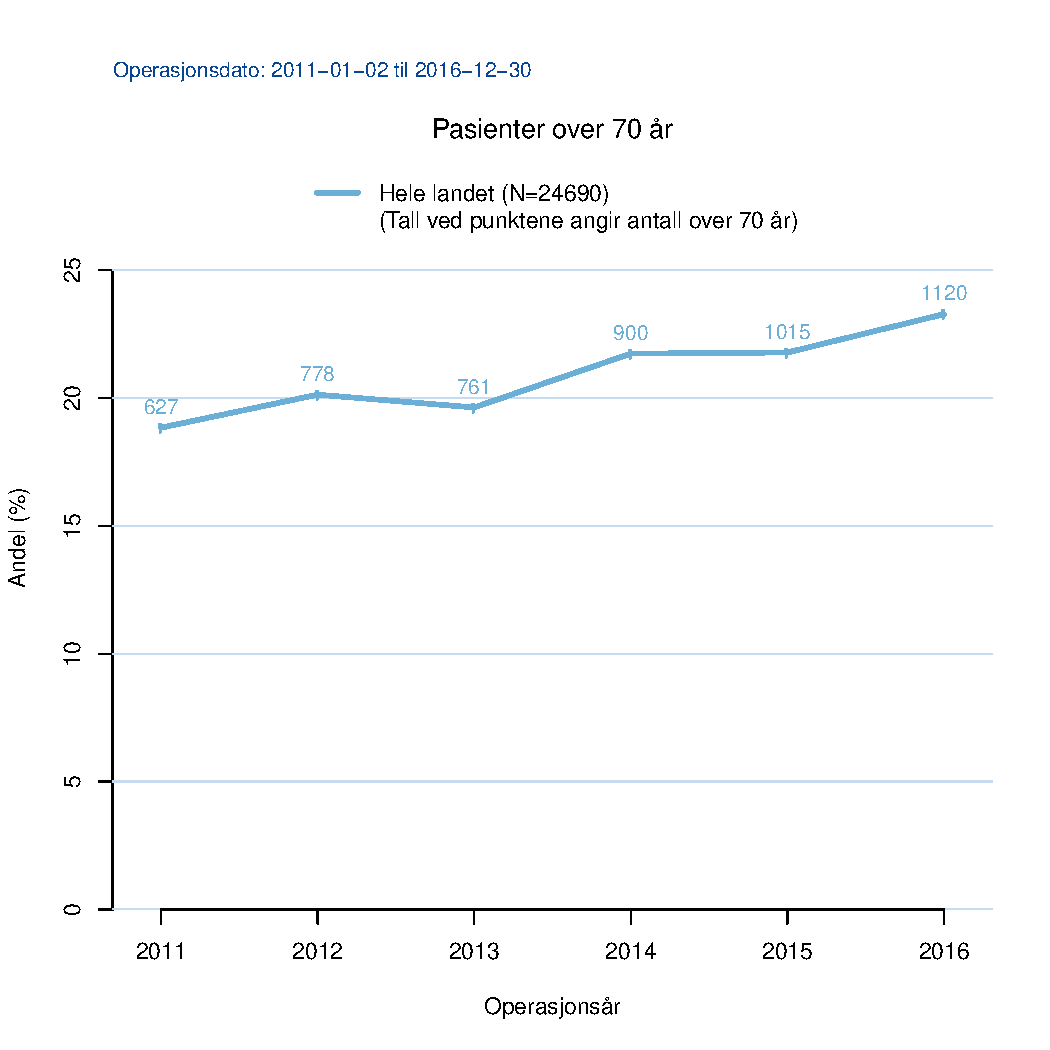
\includegraphics{Figurer/FigAlder70.pdf}}
\caption{\label{fig:Alder70} Andel ryggoperasjoner utført på personer som er 70 år eller mer.}
\end{figure}



%Figur \ref{fig:Alder} viser aldersfordeling for alle pasienter i rappAar.

%\begin{figure}[ht]
%	\centering 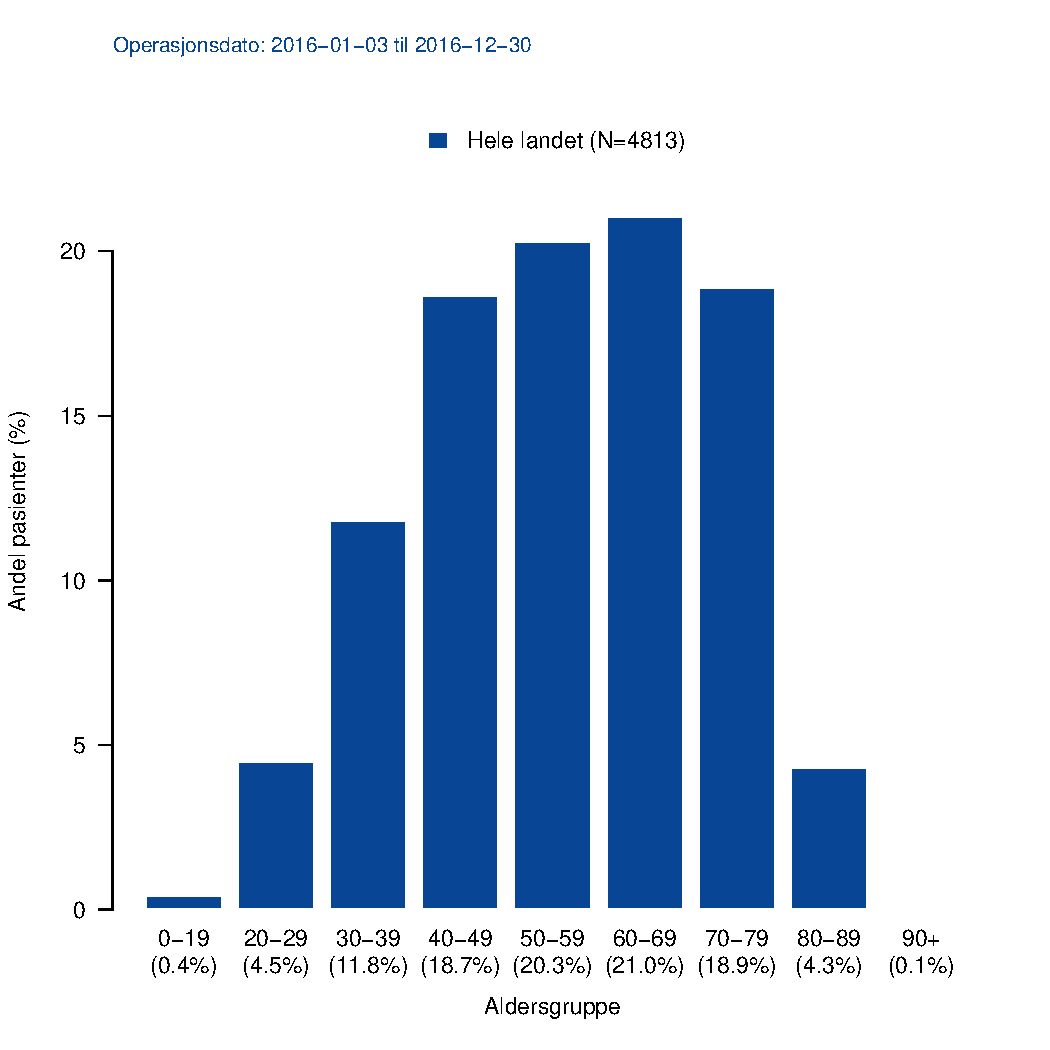
\includegraphics[width= s1\textwidth]{FigAlderFord.pdf}
%	\caption{\label{fig:Alder} paste0(AlderFord$Tittel,', ',rappAar)}
%\end{figure}

\subsection{Kroppsmasseindex (Body Mass Index, BMI)}



Opplysninger om høyde og vekt er rapportert fra pasientene selv.
Andelen pasienter med fedme har vært jevt økende fra 
20.6 \% 
i 2011
til 25.6 \%
i  2017.

Publikasjoner fra NKR viser at pasienter med fedme kan forvente signifikant mindre bedring etter 
ryggkirurgi sammenliknet med de som har lavere BMI. 




\subsection{Morsmål / etnisitet og utdanning}



Andelen fremmedspråklige (inkl. samisk) som opereres har økt fra 4.6 \% til 6.9 \% i perioden 2011 til 2017.\\
Beslutning om ryggkirurgi baserer seg på en felles forståelse mellom kirurg og
pasient av hva helseproblemene består i og hva som kan oppnås med operasjon
(«shared desicion making»). I behandling av fremmedspråklige er kommunikasjon
en utfordring. Eksempelvis var suksessraten ved lumbal prolapskirurgi for de med norsk som morsmål 65 \% mot 56 \% 
\textit{Tore sjekk tall} 
for fremmedspråklige. Bedre kommunikasjon (f.eks. ved hjelp av tolketjeneste) kan teoretisk bidra til å redusere disse
forskjellene. Figur \ref{fig:Morsmal} viser andelen fremmedspråklige operert ved de ulike avdelingene i 2017.

\begin{figure}[ht]
\scalebox{0.7}{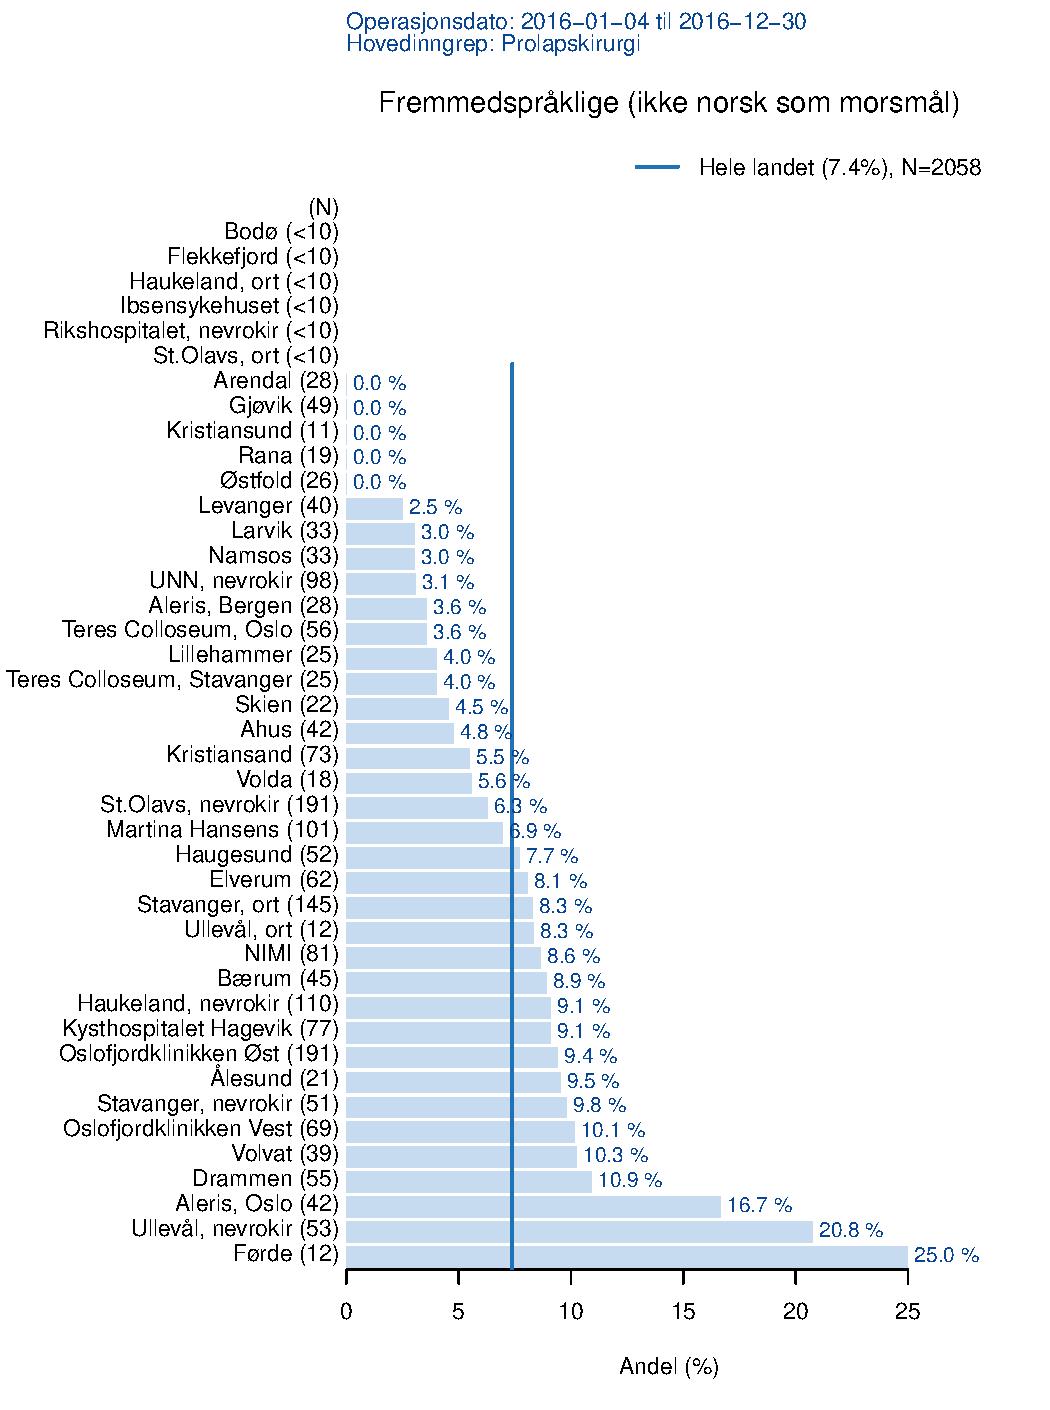
\includegraphics{Figurer/FigMorsmal.pdf}}
\caption{\label{fig:Morsmal} Andel fremmedspråklige av alle ryggopererte ved ulike sykehus i
Norge.}
\end{figure}




Lav utdanning er assosiert til dårligere operasjonsresultat. Andelen ryggopererte med høyere utdanning (høyskole eller universitet) var 36.6 i 2017 mot  30.9 i 2011. 
Opplysningene om utdanning er rapportert av pasientene selv. 
Figur \ref{fig:HoyUtdAvd} viser andel ryggopererte 
med høyskole eller universitetsutdanning ved hvert sykehus/avdeling.


\begin{figure}[ht]
\scalebox{0.7}{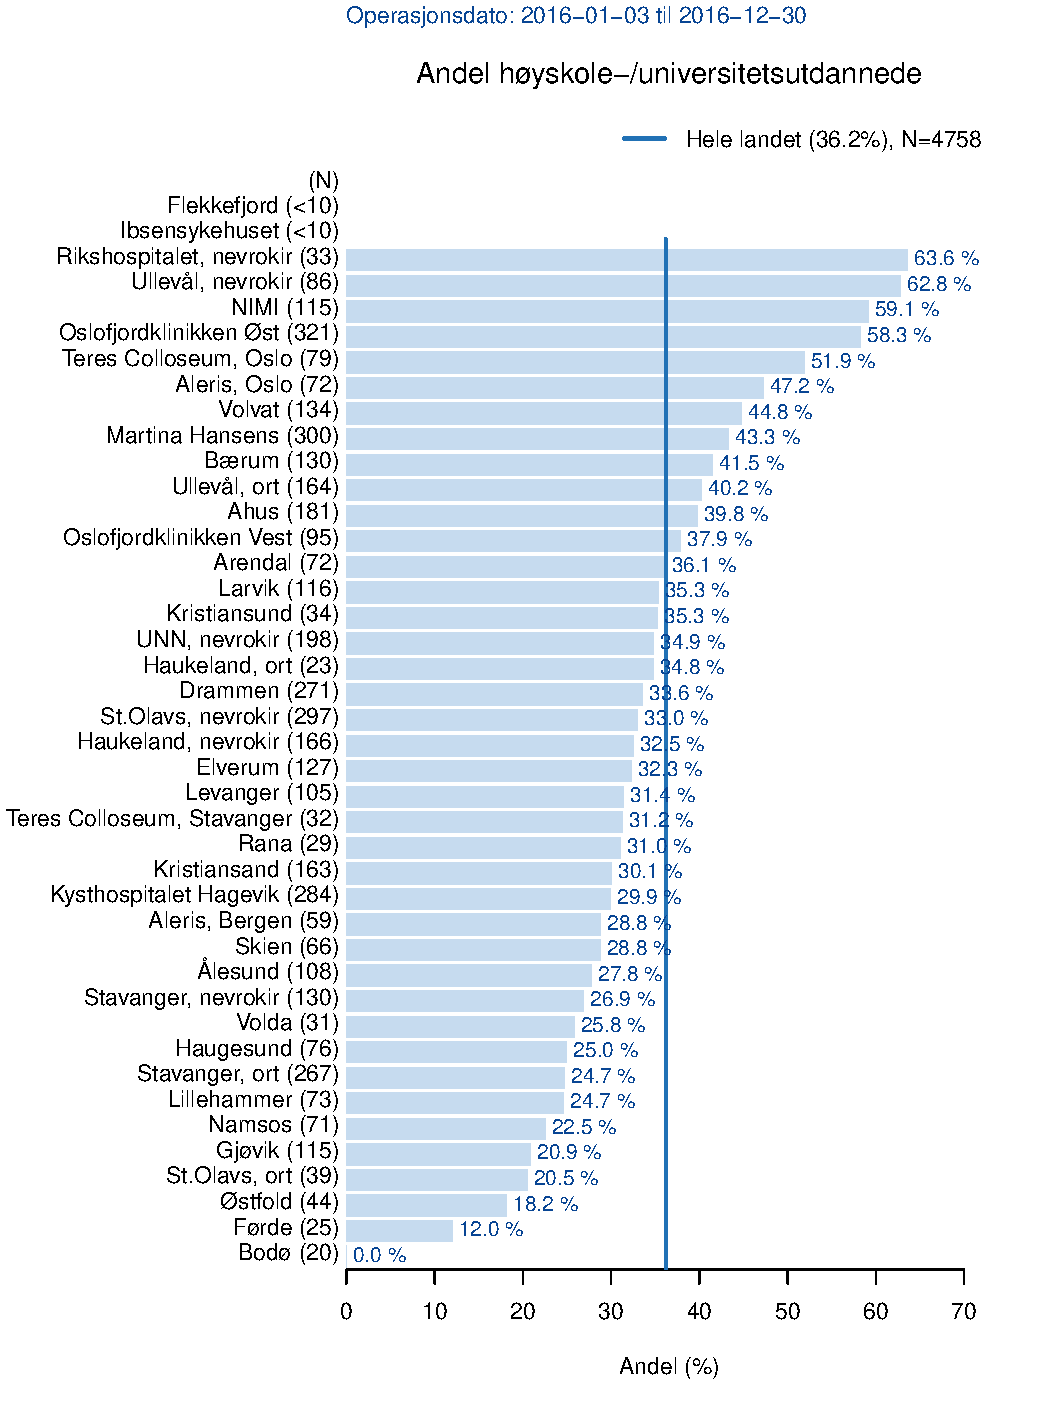
\includegraphics{Figurer/FigHoyUtdAvd.pdf}}
\caption{\label{fig:HoyUtdAvd} Andel pasienter med høyere utdanning (høyskole/universitet).}
\end{figure}


\clearpage
Avdelinger som har en pasientpopulasjon med lav utdanning og mange fremmedspråklige pasienter vil kunne forvente svakere operasjonsresultater bedømt ut fra pasient rapporterte resultatmål (PROM).
\subsection{Arbeidsstatus}
Kun  20% er i fullt arbeid når de blir ryggoperert.

% latex table generated in R 3.5.0 by xtable 1.8-2 package
% Wed Sep 26 12:16:39 2018
\begin{table}[ht]
\centering
\begin{tabular}{lr}
  \hline
 & Andeler \\ 
  \hline
I arbeid & 19.8\% \\ 
  Hjemmeværende & 1.3\% \\ 
  Student/skoleelev & 1.3\% \\ 
  Pensjonist & 31.1\% \\ 
  Arbeidsledig & 1.5\% \\ 
  Sykemeldt & 20.6\% \\ 
  Aktiv sykemeldt & 0.9\% \\ 
  Delvis Sykemeldt & 7\% \\ 
  Attføring/rehabiliteirng & 4.2\% \\ 
  Uføretrygdet & 12.3\% \\ 
   \hline
\end{tabular}
\caption{Arbeidsstatus, pasienter operert i 2017.} 
\label{tab:Arb}
\end{table}


Tabell \ref{tab:Arb} viser fordeling av arbeidsstatus før operasjon for de 98.5\% 
av pasientene i registeret som har svart på spørsmål om arbeidsstatus. 
Andelen pasienter som mottok sykepenger (sykemeldte, uføretrygdede eller personer 
på attføring) og av den grunn var helt eller delvis ute av jobb før operasjonen var 
45 \%. 

%\clearpage


\subsection{Uføretrygd og erstatning }




Pasienter som har en uavklart uføre eller erstatningssak vil sjeldnere komme tidlig tilbake i jobb etter operasjon og rapporterer mindre helseforbedringer etter operasjon. Sykehus som opererer en høy andel av denne pasientkategorien vil følgelig få dårligere resultater bedømt ut fra PROM og arbeidstilknytning.
Både andel som har søkt eller planlegger å søke uføretrygd eller erstatning ligger stabilt og var i 2017 
henholdsvis 4.7 \% og 4.5 \%. 
Figur \ref{fig:Ufor} viser andel ryggopererte ved hver avdeling som har søkt eller planlegger å søke uføretrygd.

\begin{figure}[ht]
\scalebox{0.7}{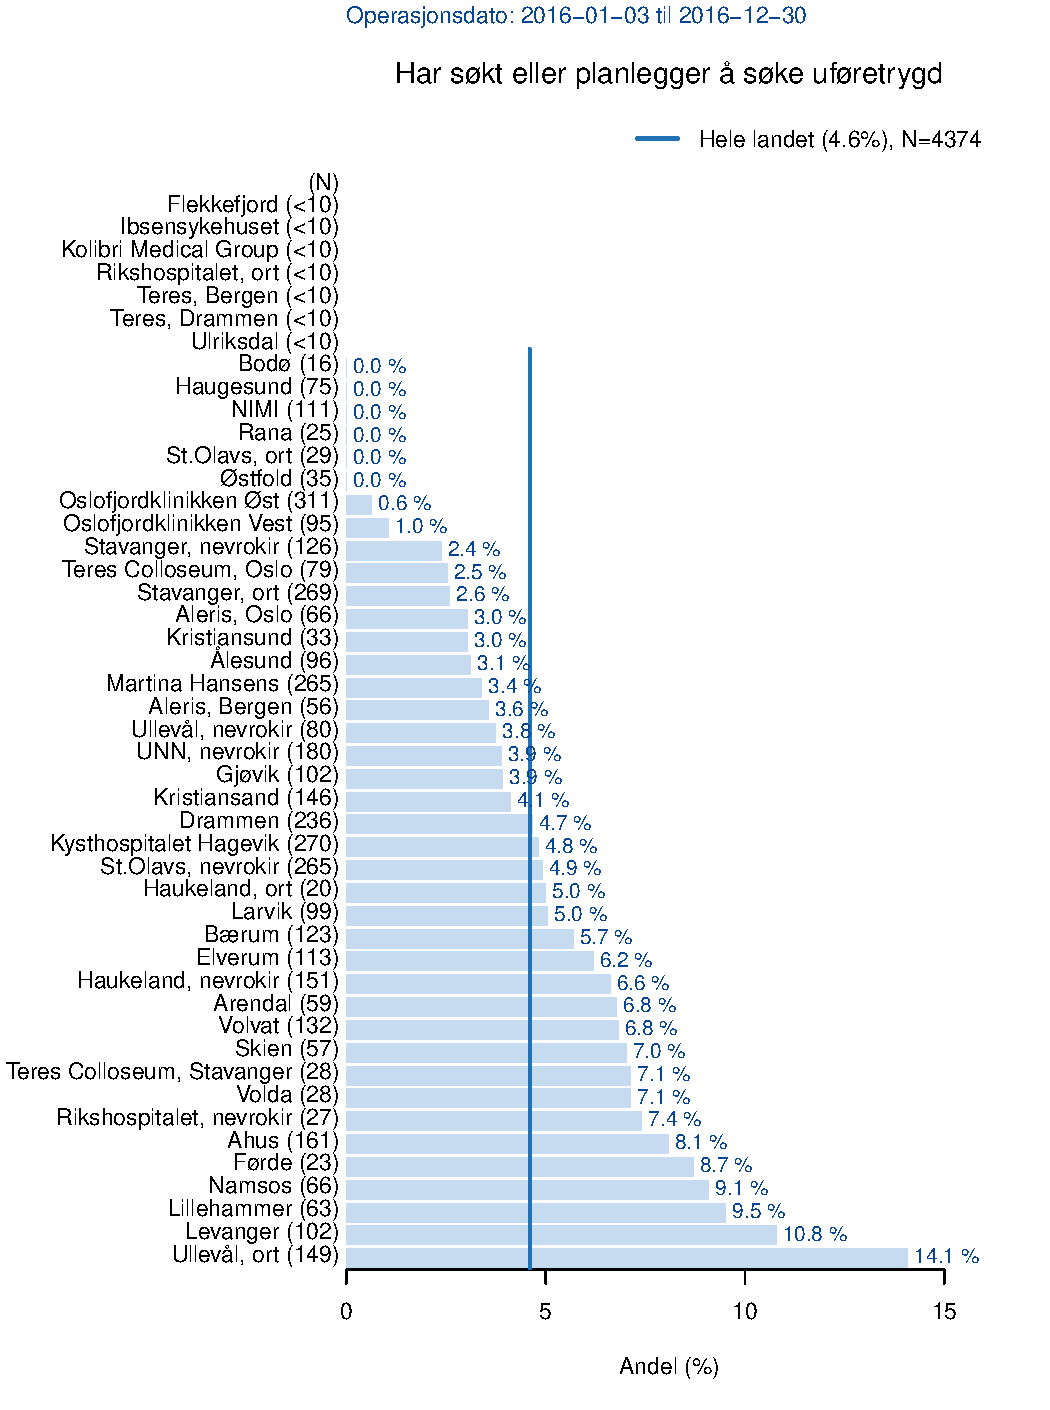
\includegraphics{Figurer/FigUforAvd.pdf}}
\caption{\label{fig:Ufor} Andel pasienter som har søkt eller planlegger å søke uføretrygd i 2017} 
\end{figure}


\clearpage

\subsection{Tidligere ryggoperert}
Informasjonen er hentet fra legeskjema.
%Figur \ref{fig:TidlOp} viser en prosentvis fordelig mellom primæroperasjon, det vil si første gangs 
%operasjon, og operasjoner hos pasienter som har vært operert tidligere.  
%Søylene representerer hvert år frem til i dag. Tallet på toppen av søylen viser antall operasjoner utført 
%det aktuelle året. 
Reoperasjoner har generelt dårligere effekt enn første gangs operasjon.





Andelen reoperasjoner var 25 \% i 2011 og 27 \% i 2017.
Av de pasientene operert i 2017 som hadde vært operert tidligere, var 57.6\% 
operert i samme nivå, 33.7\% 
operert i annet nivå og 8.6\% 
operert i både samme og annet nivå.




NKR har tidligere vist at multiple reoperasjoner har minimal effekt. Andelen som har vært operert 
mer enn 2 ganger tidligere ligger mellom 0.9 \%
og 1.6 \% for prolapspasienter og mellom 1.7 \%
og 3.1 \% for lumbal spinal stenosepasienter i perioden 2011-2017. 
Det gjenstår å evaluere om undergrupper av pasientene kan ha god nytte av flere reoperasjoner og type kirurgi som kan være mest aktuell for dem.


\subsection{ASA-grad og røyking}
ASA angir pasientens fysiske ”sårbarhet” ved anestesi og operasjon på en skala fra 1 til 5. 
Opplysningene hentes fra legeskjema.
% latex table generated in R 3.5.0 by xtable 1.8-2 package
% Wed Sep 26 12:16:45 2018
\begin{table}[ht]
\centering
\begin{tabular}{crr}
  \hline
 & Antall & Prosent \\ 
  \hline
I & 1362 & 25.8\% \\ 
  II & 3090 & 58.6\% \\ 
  III & 784 & 14.9\% \\ 
  IV & 10 & 0.2\% \\ 
  V & 1 & 0\% \\ 
  Ikke besvart & 25 & 0.5\% \\ 
   \hline
\end{tabular}
\caption{Fordeling av ASA-grad, operasjoner utført i 2017} 
\label{tab:ASA}
\end{table}


Tabell \ref{tab:ASA} viser fordeling av ASA grad. Andelen pasienter med ASA grad I-II 
var 84.4\%. Pasienter som røyker, havner 
automatisk i ASA-grad II eller høyere. Data fra NKR har vist at røyking er assosiert til dåligere operasjonsresultat.
Mange kirurger krever eller anbefaler røykeslutt før mer omfattende inngrep slik som fusjonskirurgi.
%txt
Andel røykere som ryggopereres har gått ned fra 28.2 \% i 2011 til 19.1 \% i 2017. 



\subsection{Radiologisk utredning}

Tabell \ref{tab:RV} viser hvor stor andel av pasientene som har vært til ulike typer 
radiologisk undersøkelser. En pasient kan ha vært til flere undersøkelser. Hyppigste radilologiske diagnoser er skiveprolaps og spinal stenose.
Spørsmålene er besvart av leger. 

% latex table generated in R 3.5.0 by xtable 1.8-2 package
% Wed Sep 26 12:16:47 2018
\begin{table}[ht]
\centering
\begin{tabular}{lrr}
  \hline
 & Antall & Andeler \\ 
  \hline
CT & 371 & 7\% \\ 
  MR & 5175 & 98\% \\ 
  Radikulografi & 38 & 1\% \\ 
  Diskografi & 2 & 0\% \\ 
  Diagnostisk blokade & 28 & 1\% \\ 
  Røntgen LS-columna & 1208 & 23\% \\ 
  Med fleksjon/ekstensjon & 394 & 7\% \\ 
  Tot. ant. & 5272 &   \\ 
   \hline
\end{tabular}
\caption{Radiologisk vurdering, 2017} 
\label{tab:RV}
\end{table}




Tabell \ref{tab:RF} viser diagnoser basert på radiologiske funn hos alle pasienter 
i 2017. 
Spørsmålene er besvart av leger.
En pasient kan ha flere diagnoser.
%txtRFnorm


% latex table generated in R 3.5.0 by xtable 1.8-2 package
% Wed Sep 26 12:16:47 2018
\begin{table}[ht]
\centering
\begin{tabular}{lrr}
  \hline
 & Antall & Andeler \\ 
  \hline
Skiveprolaps & 2346 & 44\% \\ 
  Sentral spinalstenose & 1755 & 33\% \\ 
  Lateral spinalstenose & 1771 & 34\% \\ 
  Foraminal stenose & 636 & 12\% \\ 
  Degenerativ rygg/skivedegenerasjon & 926 & 18\% \\ 
  Istmisk spondylolistese & 143 & 3\% \\ 
  Degenerativ spondylolistese & 521 & 10\% \\ 
  Degenerativ skoliose & 155 & 3\% \\ 
  Synovial syste & 144 & 3\% \\ 
  Pseudomeningocele & 1 & 0\% \\ 
  Tot.ant. & 5272 &   \\ 
   \hline
\end{tabular}
\caption{Radiologiske diagnoser, 2017} 
\label{tab:RF}
\end{table}





\section{Virksomhetsdata}

Andelen som er operert ved hjelp av synsfremmende midler (mikroskop eller
lupebriller), som har åpenbare fordeler, har økt fra 86 \% i 2011 til 
98 \% i 2017 for lumbalt prolaps. 
Tilsvarende tall for lumbal spinal stenose var en økning fra 68 \% i 2011 til 
98 \% i 2017.



\subsection{Type operasjon}



De hyppigste tilstandene pasienter ble operert for i 2017 var lumbalt prolaps (41 \%) og spinal stenose (42 \%). Tabell \ref{tab:AntHovedInngrep} viser fordeling av hovedinngrepstype, samt antall registrerte operasjoner for hver hovedinngrepstype.
''Foramenotomi'' betyr at det er gjort dekompresjon for lumbal spinal stenose med bevaring av midtlinjestrukturer. 

% latex table generated in R 3.5.0 by xtable 1.8-2 package
% Wed Sep 26 12:16:47 2018
\begin{table}[ht]
\centering
\begin{tabular}{lrr}
  \hline
 & Antall & Andeler \\ 
  \hline
Udefinerbart & 161 & 3\% \\ 
  Prolapskirurgi & 2161 & 41\% \\ 
  Foramenotomi & 2087 & 40\% \\ 
  Laminektomi & 191 & 4\% \\ 
  Interspin. implantat & 1 & 0\% \\ 
  Fusjonskirurgi & 598 & 11\% \\ 
  Skiveprotese & 45 & 1\% \\ 
  Rev. av implantat & 28 & 1\% \\ 
   \hline
\end{tabular}
\caption{Fordeling av hovedinngrep, 2017} 
\label{tab:AntHovedInngrep}
\end{table}



%\begin{figure}[ht]
%      \scalebox{s1}{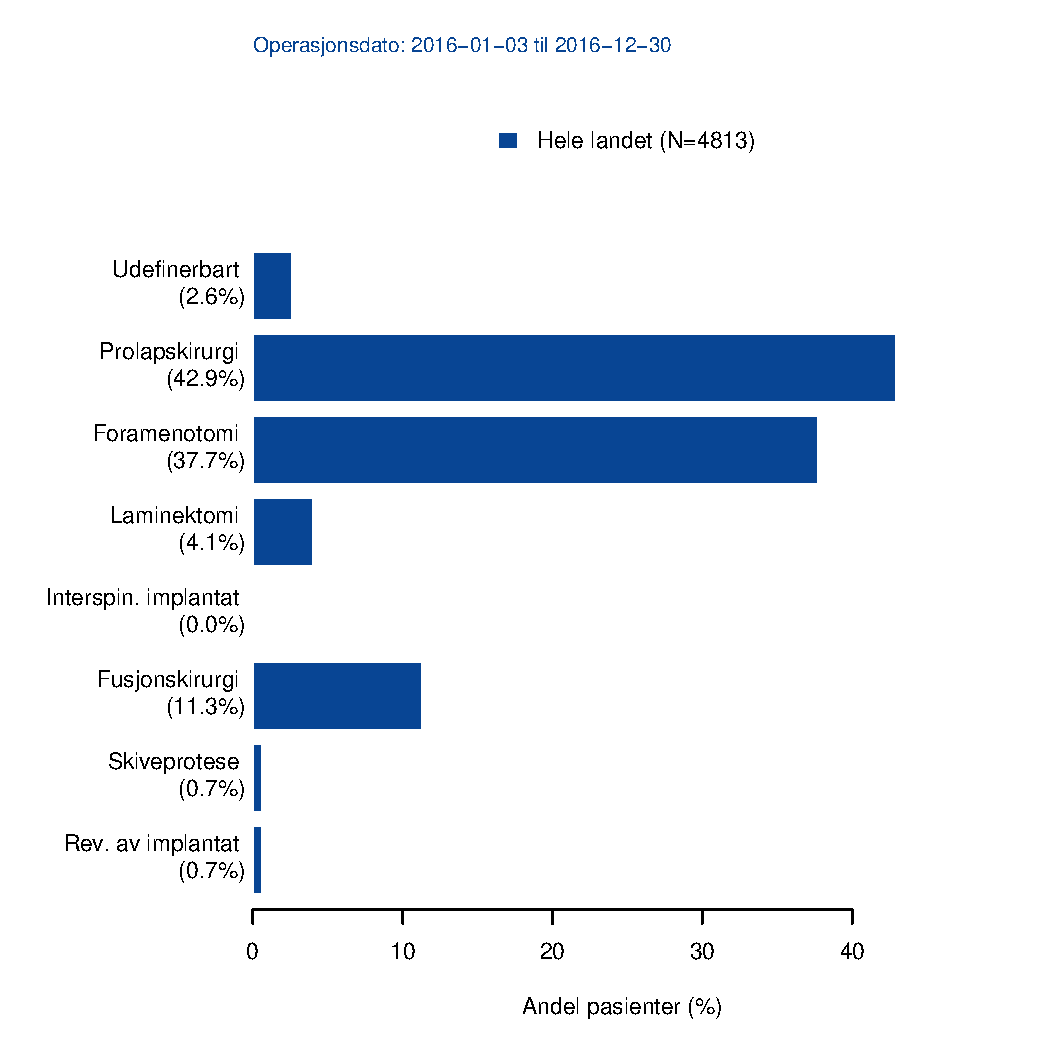
\includegraphics{Figurer/HovedInngrep.pdf}}
%      \caption{\label{fig:HovedInngrep} HovedInngrep$Tittel}
%\end{figure}



\subsubsection{Degen. spondylolistese operert med fusjonskirurgi}


I 2017 hadde 18.3 \% av de som ble operert for spinal stenose  også en forskyvning mellom ryggvirvlene (Degenerativ spondylolistese). I internasjonal litteratur er det sprikende anbefalinger i forhold til om de bør få tilleggsbehandling med avstivningsoperasjon (fusjonskirurgi).
 

Norske studier basert på data fra NKR har vist at tilleggseffekten er liten og assosiert til høyere kostnader (flere liggedøgn på sykehus). 
I 2018 blir det publisert en ny studie fra NKR i samarbeid med  tilsvarende registre i Sverige og Danmark. Denne viser stor forskjell i bruk av fusjonskirurgi mellom landene og at denne tilleggbehandlingen ikke er assosiert til større behandlingseffektivitet, men økte kostnader. En pågående nasjonal RCT multisenter studie skal i samarbeid med NKR evaluere om undergrupper av pasientene med spinal stenose og degenerativ spondylolistese kan ha spesiell nytte av fusjonskirurgi.
\clearpage

Figur \ref{fig:degSponFusj} viser at det er stor variasjon i bruk av fusjonskirurgi, 
for denne pasientgruppen, også mellom avdelinger på samme sykehus. Nevrokirurgiske avdelinger bruker mindre fusjonskirurgi enn de ortopediske.
\begin{figure}[ht]
\scalebox{0.7}{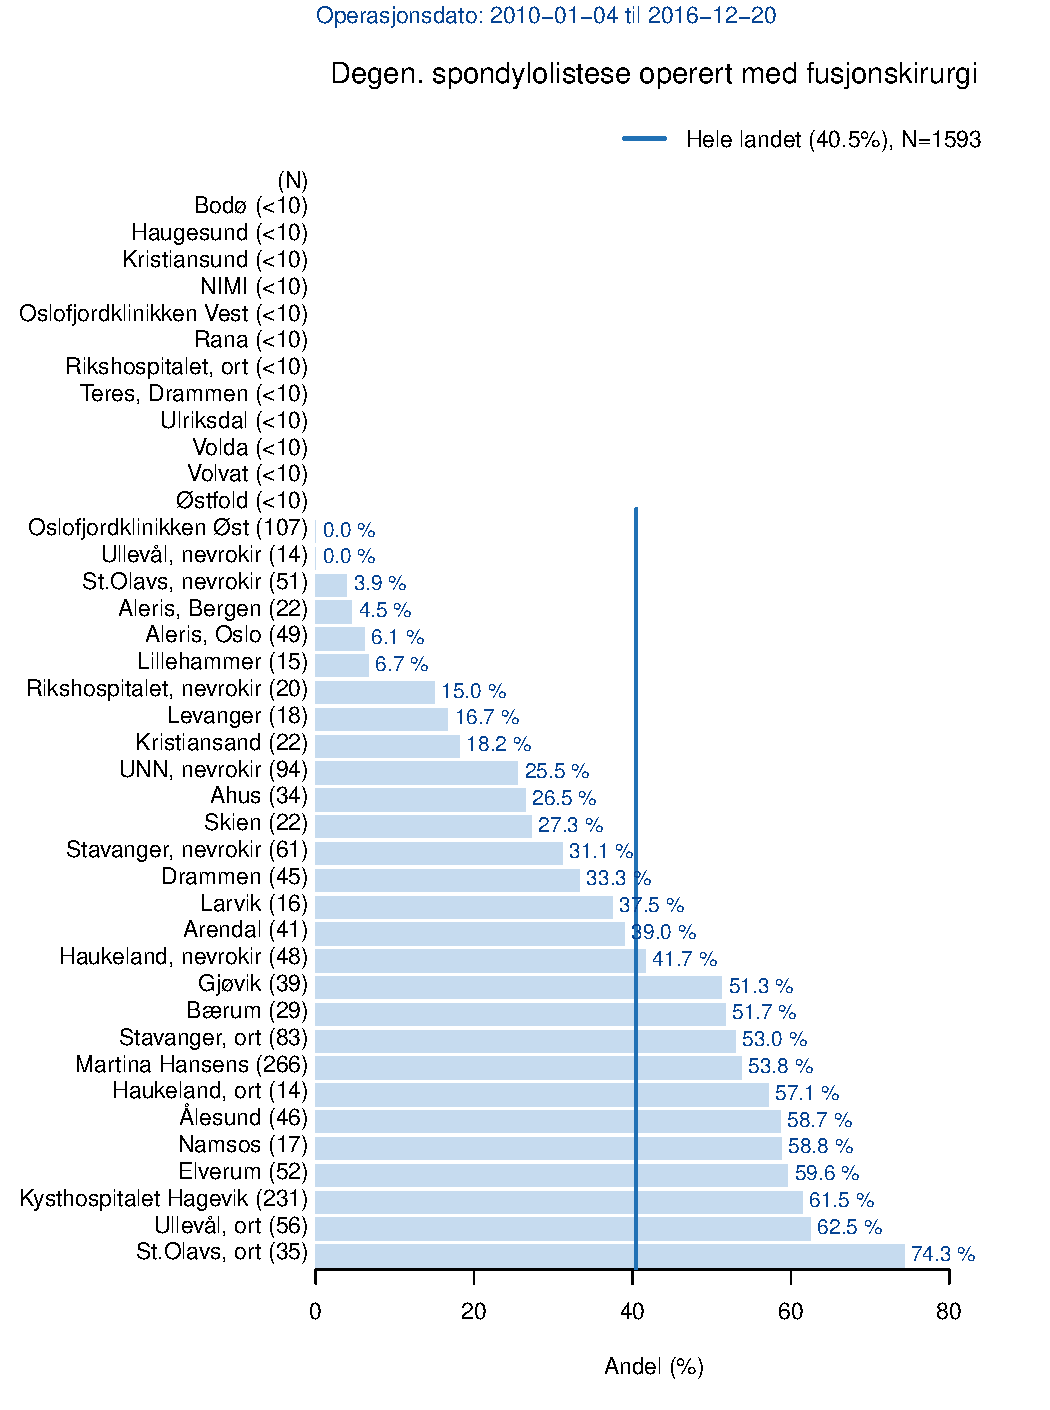
\includegraphics{Figurer/FigdegSponFusj.pdf}}
\caption{\label{fig:degSponFusj} Lumbal spinal stenose og degenerativ spondylolistese operert med fusjonskirurgi}
\end{figure}

Figur \ref{fig:degSponFusjSStid} viser at andelen som får 
tilleggsbehandling med fusjonskirurgi er redusert fra 50.9 \% 
i 2011 til 29.7 \% i 2017.

\begin{figure}[ht]
\scalebox{0.7}{\includegraphics{Figurer/FigdegSponFusjSStid.pdf}}
\caption{\label{fig:degSponFusjSStid} Andel pasienter med degenerativ spondylolistese og spinal stenose som blir operert med fusjonskirurgi per år}
\end{figure}



\clearpage


\subsection{Liggetid}

Informasjonen er hentet fra legeskjema.
%Figur \ref{fig:Liggedogn} viser liggedøgnsfordeling for alle pasienter operert i rappAar. 
%Figur \ref{fig:LiggedognTid} viser gjennomsnittlig antall liggedøgn per år.  
Det har vært en reduksjon i liggetid  på sykehus (ca 1 døgn) fram til 2017 for både lumbal prolaps og spinal stenose opererte. 
Dette kan henge sammen med økt bruk av mindre invasive operasjonsmetoder og mer dagkirurgi. 
Andelen operert med dagkirurgi for hhv lumbalt skiveprolaps og spinal stenose har gått opp fra 
23 \% og 9 \%  i 2011 til 31 \% og 13 \%  i 2017  
Figur \ref{fig:LiggetidAvdPro} og \ref{fig:LiggetidAvdSS} viser at det var stor variasjon i antall liggedøgn mellom sykehus og avdelinger i 2017.


      
      
      
      %\begin{figure}[h] 
%\scalebox{s1}{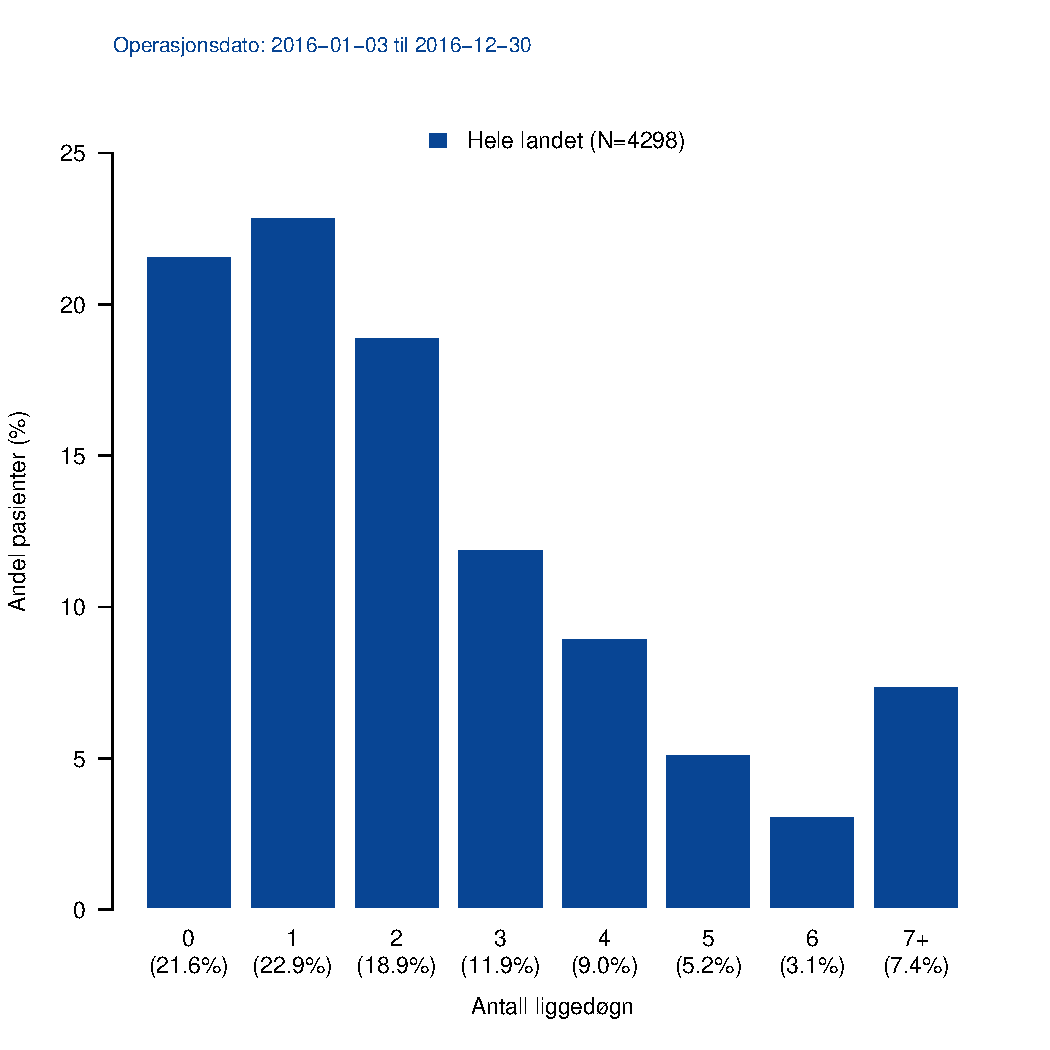
\includegraphics{Figurer/FigLiggetidFord.pdf}}
%\caption{LiggetidFord$Tittel}
%\label{fig:Liggedogn}
%\end{figure}

% \begin{figure}[h] 
% \centerline{
      % \scalebox{s2}{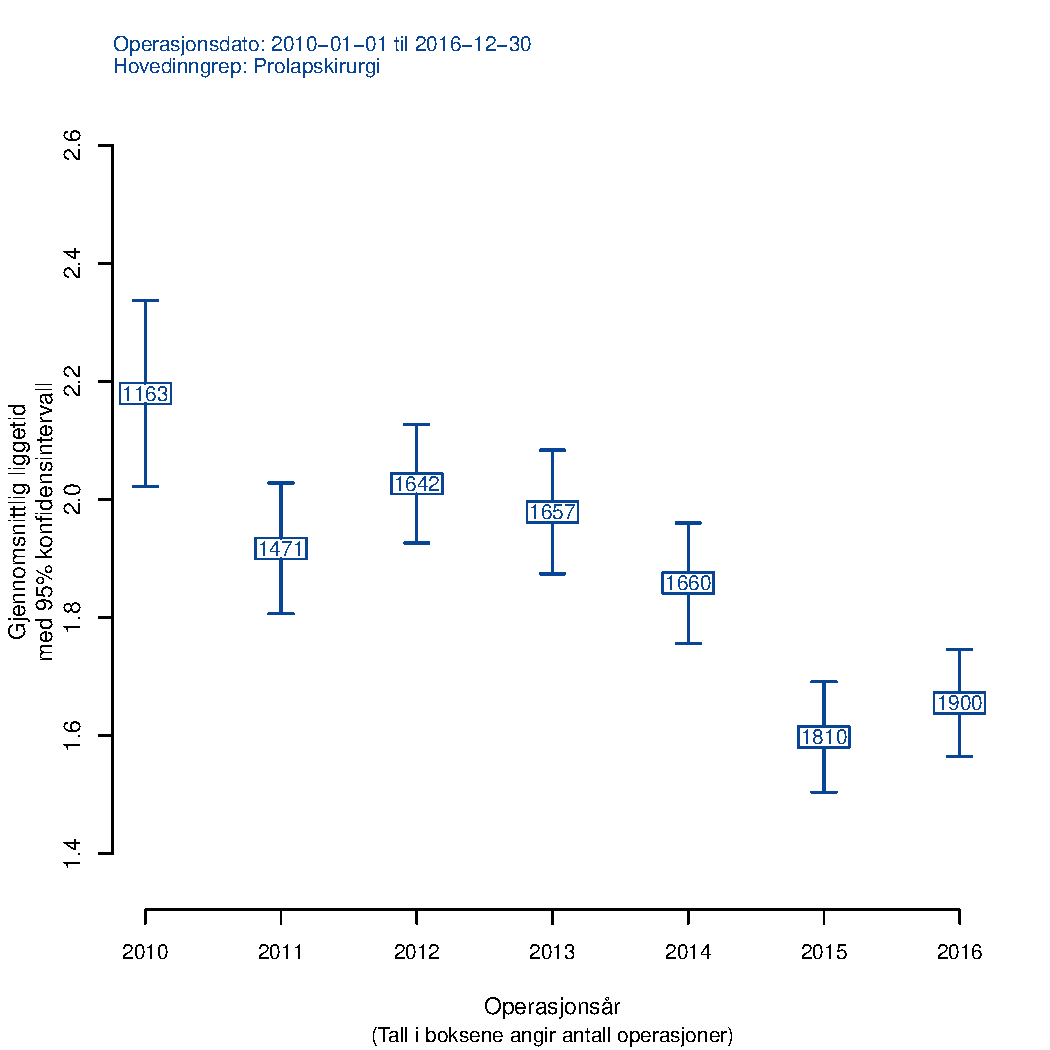
\includegraphics{Figurer/LiggetidBoxPro.pdf}}
      % \scalebox{s2}{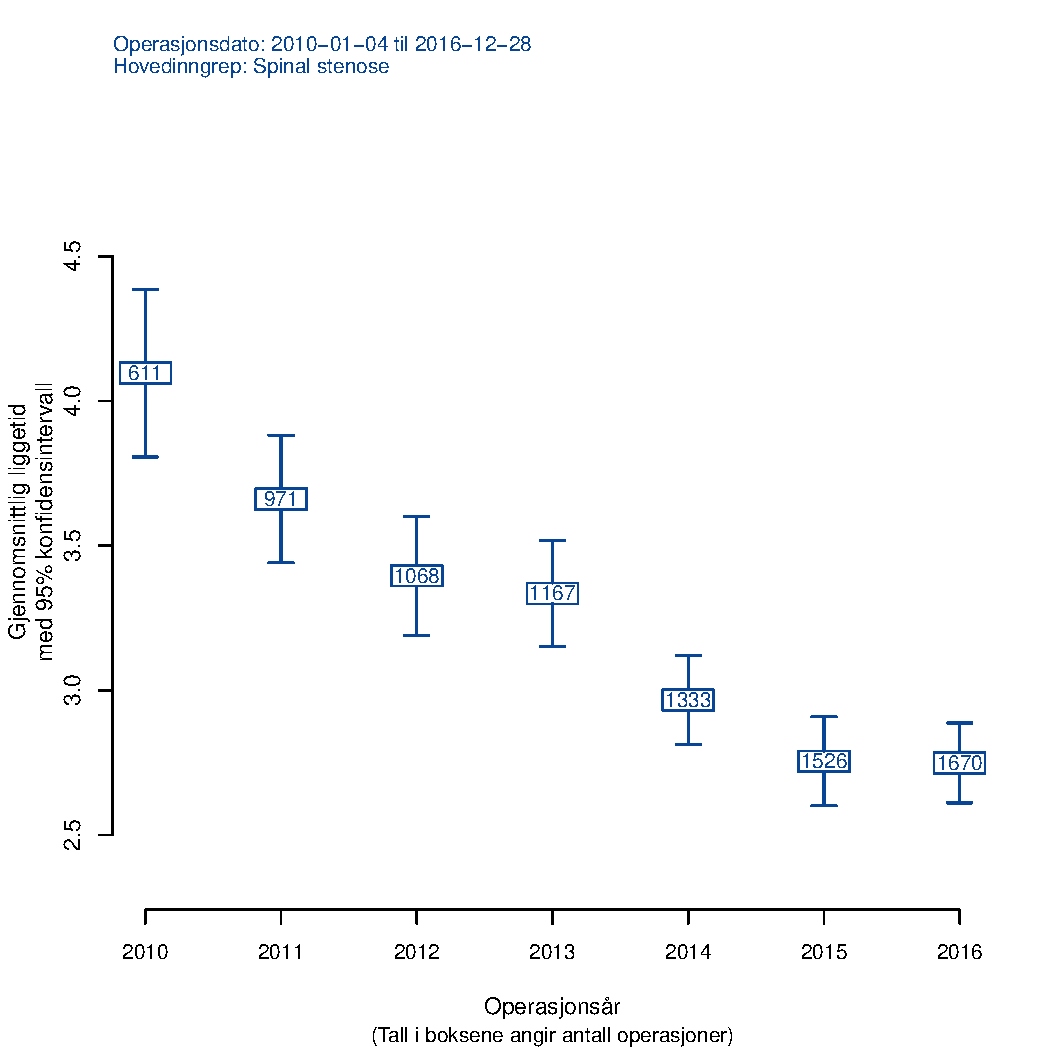
\includegraphics{Figurer/LiggetidBoxSS.pdf}}
      % }
% \caption{Gjennomsnittlig liggetid for hhv. lumbalt prolaps og spinal stenose. }
% \label{fig:LiggedognTid}
% \end{figure}

\begin{figure}[h] 
\scalebox{0.7}{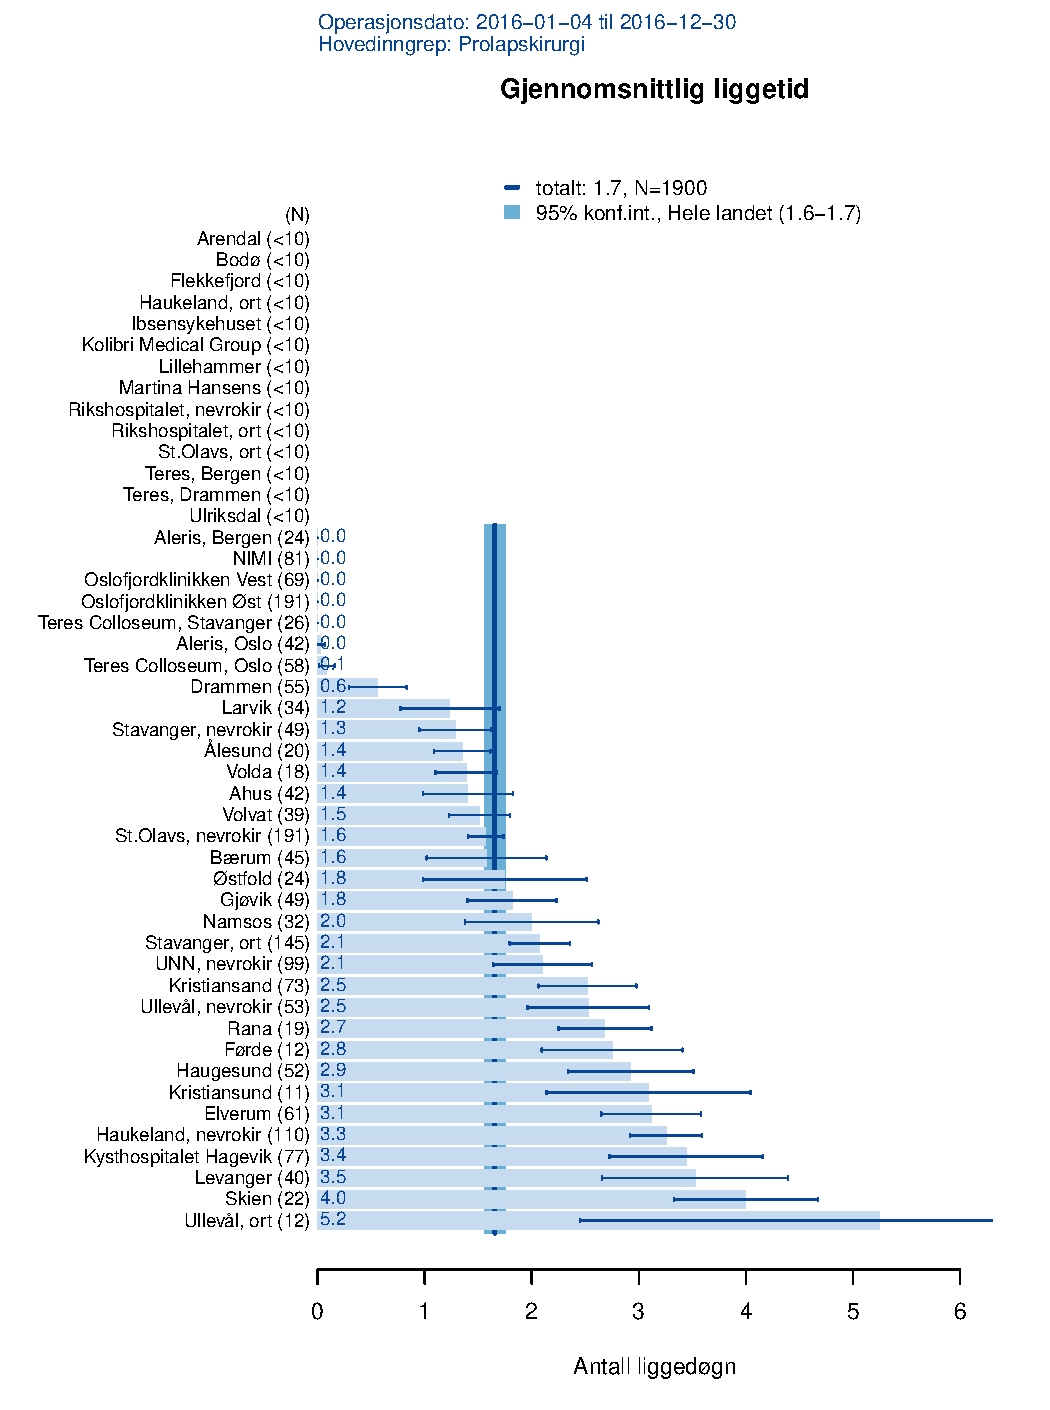
\includegraphics{Figurer/LiggetidAvdPro.pdf}}
\caption{Gjennomsnittlig liggetid for lumbalt prolaps ved ulike avdelinger i 2017. } 
\label{fig:LiggetidAvdPro}
\end{figure}

\begin{figure}[h] 
\scalebox{0.7}{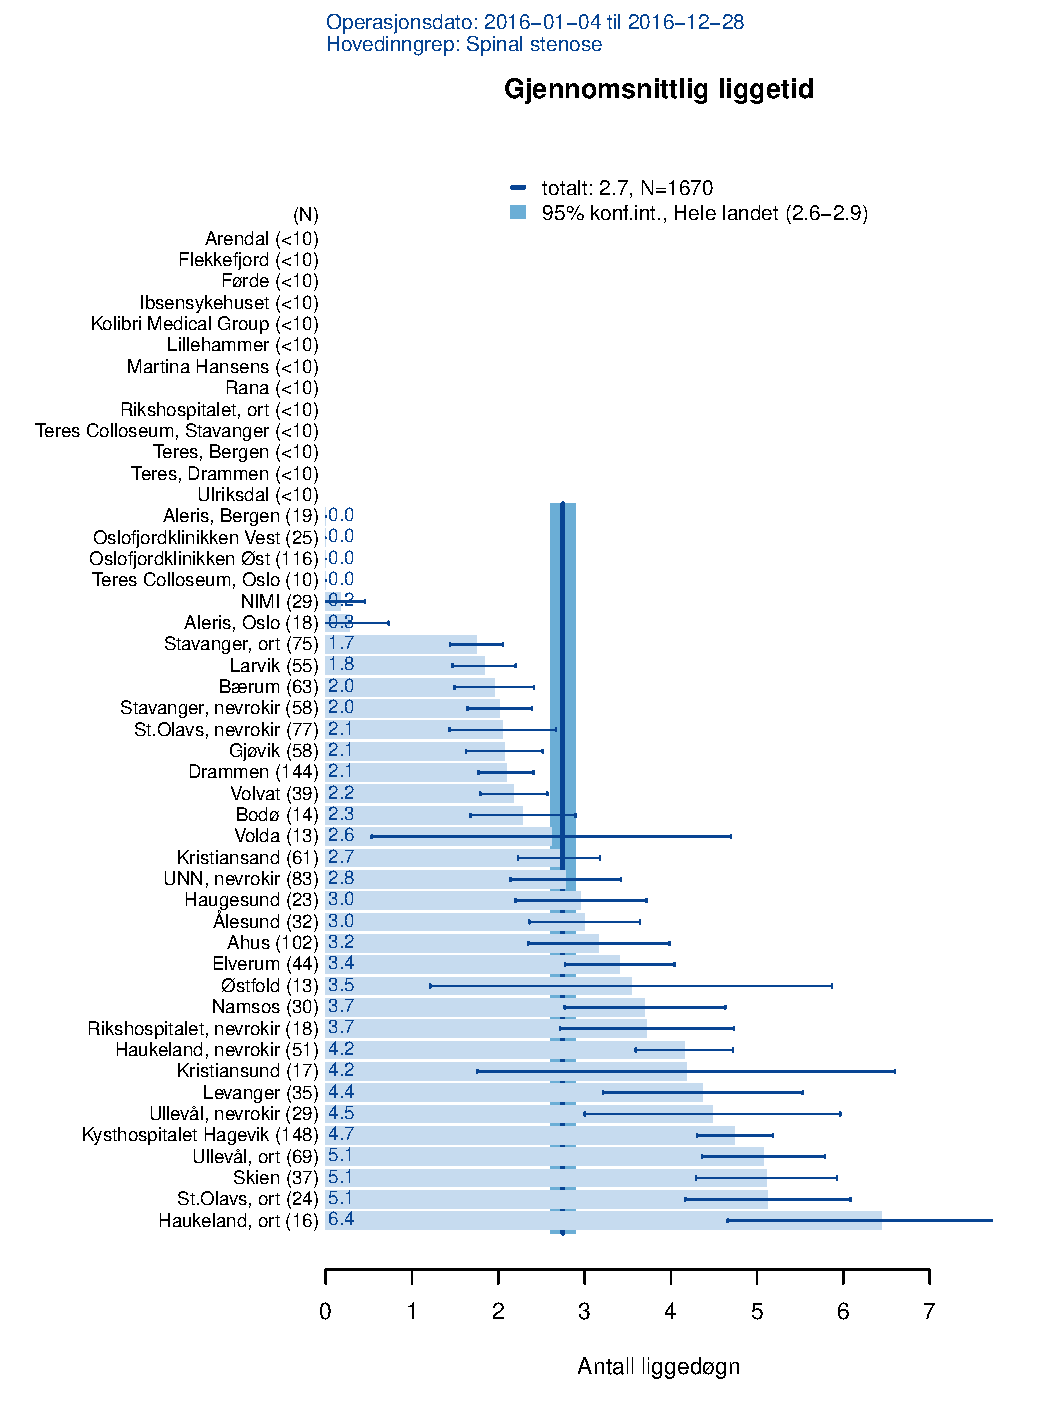
\includegraphics{Figurer/LiggetidAvdSS.pdf}}
\caption{Gjennomsnittlig liggetid for lumbal spinal stenose ved ulike avdelinger i 2017 } 
\label{fig:LiggetidAvdSS}
\end{figure}


      
      
      
      
      \clearpage

\section{Resultatmål}
All informasjon i dette kapitlet er hentet fra pasientskjema.  Viktige årsaker til variasjon i operasjonsresultat kan være at sykehusene behandler
ulike pasientgrupper med ulik risikoprofil. Ingen av resultatmålene er justert
for disse forskjellene. Noen risikofaktorer kan modifiseres/bedres gjennom bedre styring og planlegging av
virksomheten, strengere indikasjonsstilling og bedret pasientsikkerhet. Andre faktorer, for eksempel utdanningsnivå, lar seg ikke modifisere.
Sammenholdt med bakrunnsdata og virksomhetsdata kan resultatmålene imidlertid gi en pekepinn på hvor godt behandlingstilbudet fungerer på ulike sykehus. Indikasjonsstillingen («inngangsbilletten»)til kirurgi er mest avgjørende for om operasjonsresultatet blir vellykket: Fikk rett person, rett
behandling til rett tid?

Resultatmålene er utviklet gjennom forskning (valideringsstudier) i regi av NKR i samarbeid
med blant annet Nasjonalt kompetansesenter for rygg og nakke kirurgi og ulike universistessykehus i Norge. Noen få er hentet fra annen
internasjonal litteratur. De terskelverdiene som brukes er med andre ord forskningsbaserte.
 
\textbf{Det er viktig å merke seg at pasienter som er operert i 2016 først får resultater fra ettårs oppfølgning i 2017.} 


      
      


      
      \subsection{ Resultater etter ryggkirurgi, 2011 til 2017}

\subsection{Oswestry Disability Index (ODI)}


      
      
      
      ODI brukes som hovedeffektmål og uttrykker smerterelatert  fysisk funksjon i dagliglivets aktiviteter og sykdomsspesifikk livskvalitet hos ryggpasienter. Skalaen går fra 0
til 100, hvor 0 angir ingen funksjonshemming og følgelig beste livskvalitet.

I tillegg angir pasienten smerteintensitet i henholdsvis ben og rygg på en numerisk smerteskala (NRS), 
fra 0 (ingen smerte) til 10 (verst tenkelige smerte).
\\

Gjennomsnittlig ODI score var 46.4 før operasjon og 16.7 ett år etter
operasjon for lumbalt prolaps i 2016. Dette betyr at funksjonssvikten ble redusert 
fra alvorlig til minimal for gjennomsnittspasienten. 
Pasienter operert for lumbal spinal stenose fikk også
betydelig bedring (ODI redusert fra 39.2 (betydelig funksjonssvikt) til 23.2) (lett til moderat funksjonssvikt) ett år etter kirurgi. 
De som ble operert med fusjonkirurgi har
omtrent samme forbedring (ODI redusert fra 42.0 til 25.1). Resultatene synes å være omtrent de samme fra år til år. Suksessrate, det vil si forbedring av ODI på mer enn 20 poeng, ligger stabilt rundt 60 \% for prolapspasienter, ett år etter operasjon. 
For spinal stenosepasienter ligger "suksessraten" ett år etter operasjon (forbedring av ODI på mer enn 30 \%) stabilt rundt 60\%.
Dette betyr at selv om
pasientene kan forvente en betydelig bedring, vil mange fortsatt ha en del restplager
ett år etter kirurgi. \\
 
 NKR
sammenstiller også norske resultater tilsvarende registre i Sverige og
Danmark. Indikasjonsstillen for kirurgi er lik og resultatene synes å være de samme i de tre nordiske landene.
Resultatene varierer imidlertid mye mellom sykehus og fra pasient til pasient. \\

%Figur \ref{fig:OswEndr} viser gjennomsnittlig endring av ODI fra før operasjon til ett år etter.





      
      Figurene \ref{fig:OswEndrAvdPro} og \ref{fig:OswEndrAvdSS} viser gjennomsnittlig endring 12 måneder etter for hver avdeling for henholdsvis prolaps og spinal stenose pasienter. Forskjellene er små. Vi ser også at konfidensintervallene er relativt brede og overlappende.

\begin{figure}[h] 
\scalebox{0.7}{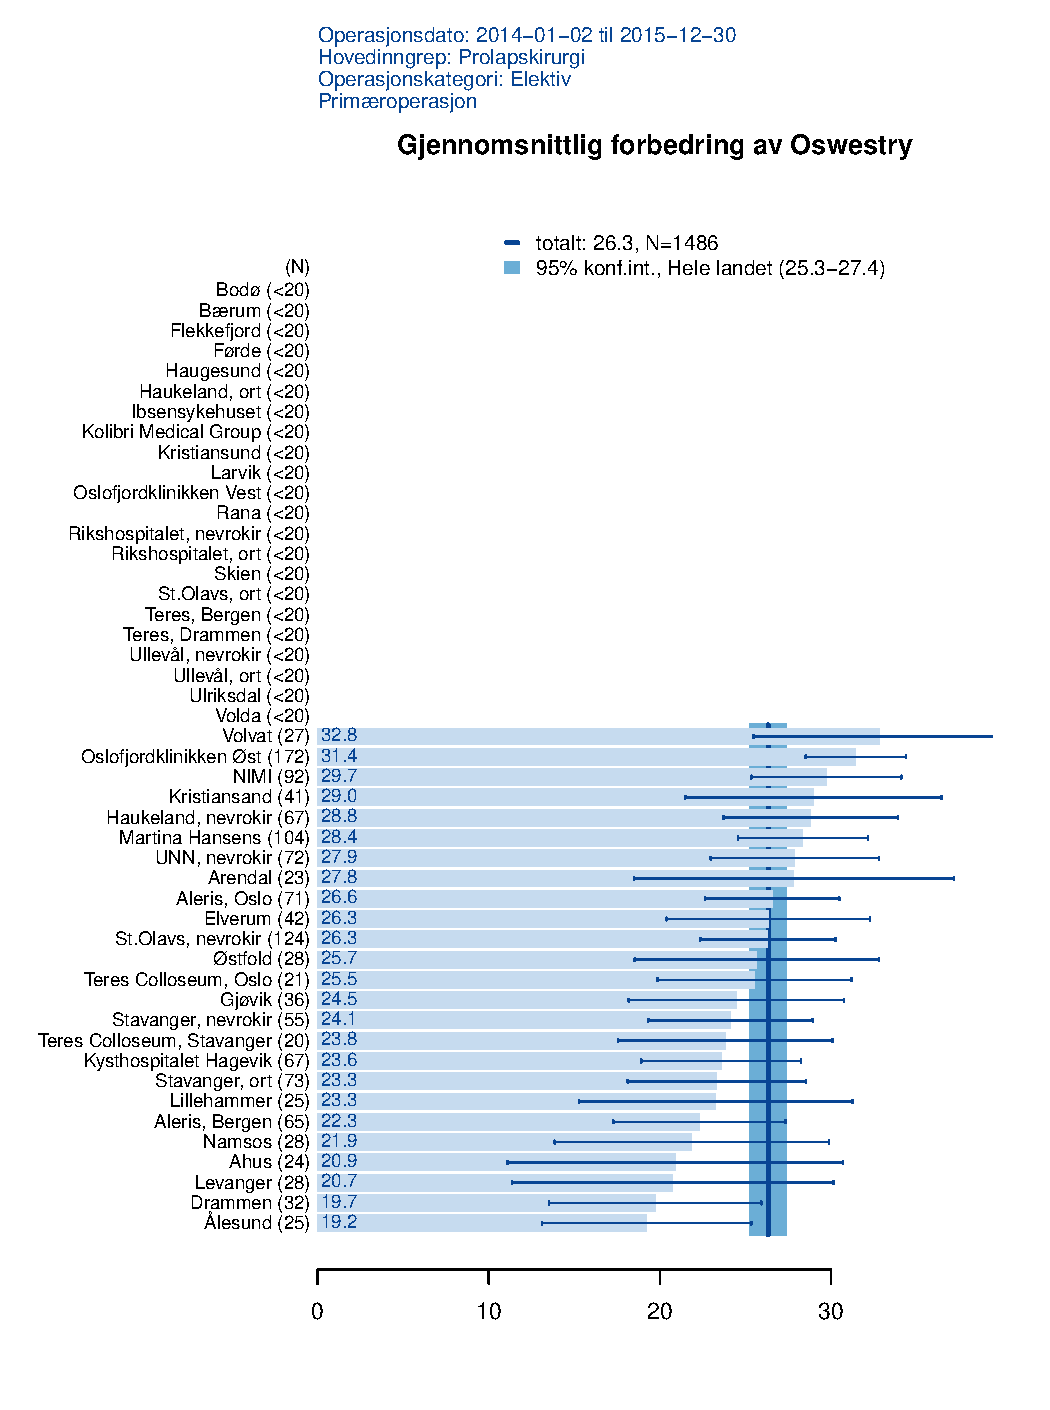
\includegraphics{Figurer/OswEndrAvdPro.pdf}}
\caption{Gjennomsnittlig endring av ODI per avdeling for lumbalt prolaps.}
\label{fig:OswEndrAvdPro}
\end{figure}

\begin{figure}[h] 
\scalebox{0.7}{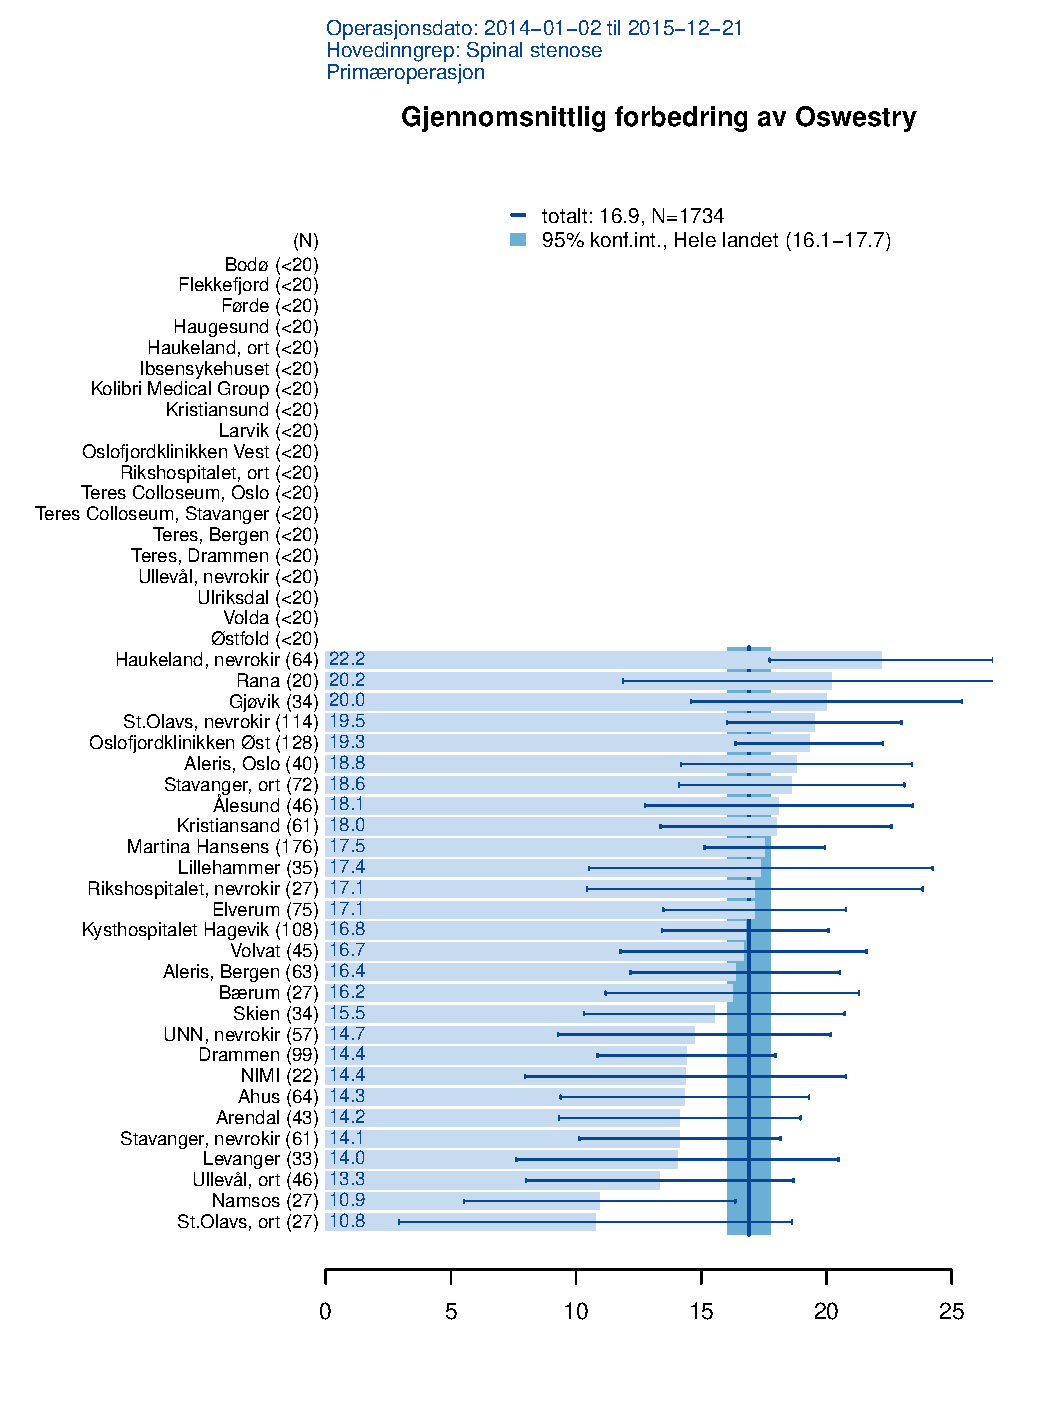
\includegraphics{Figurer/OswEndrAvdSS.pdf}}
\caption{Gjennomsnittlig endring av ODI per avdeling for spinal stenose.}
\label{fig:OswEndrAvdSS}
\end{figure}



\clearpage


ODI skår under eller lik 22 poeng oppleves av de fleste pasientene som et godt og helt akseptabelt fysisk funksjonsnivå 12 mnd etter ryggopersjon. Figurene \ref{fig:Osw22Pro} og \ref{fig:Osw22SS} angir hvor stor andel av henholdsvis prolaps og spinal stenose opererete som oppnår dette.

\begin{figure}[ht]
\scalebox{0.7}{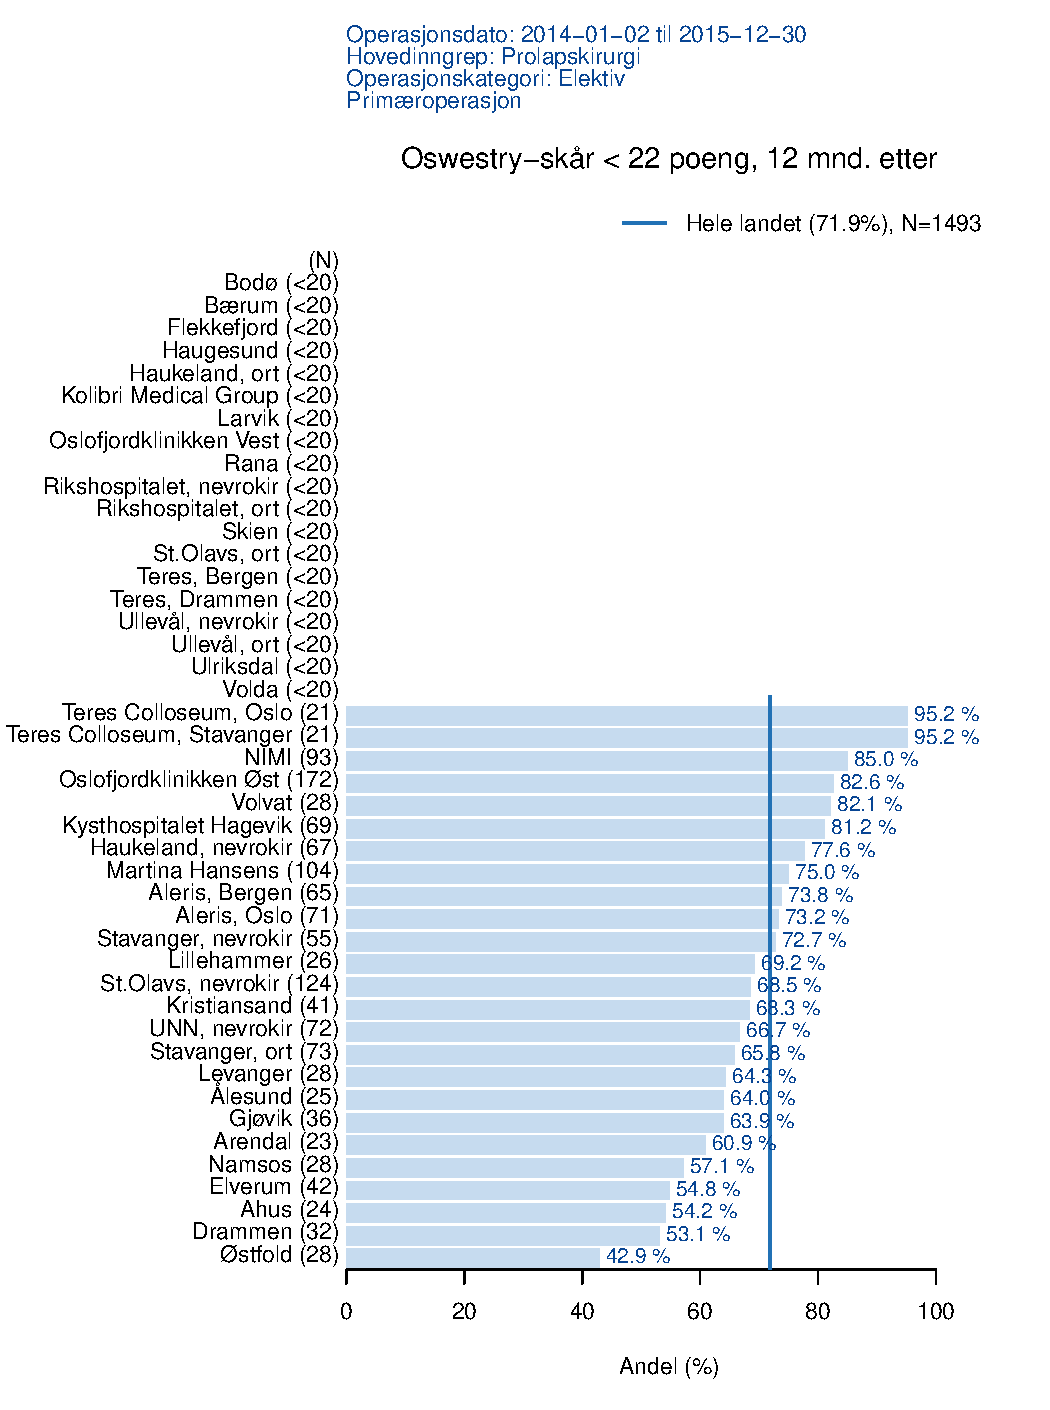
\includegraphics{Figurer/FigOsw22Pro.pdf}}
\caption{\label{fig:Osw22Pro}   Andel pasienter med ODI under 22 ett år
      etter prolapsoperasjon. Pasienter operert i 2015 og 2016.}
\end{figure}

\begin{figure}[ht]
\scalebox{0.7}{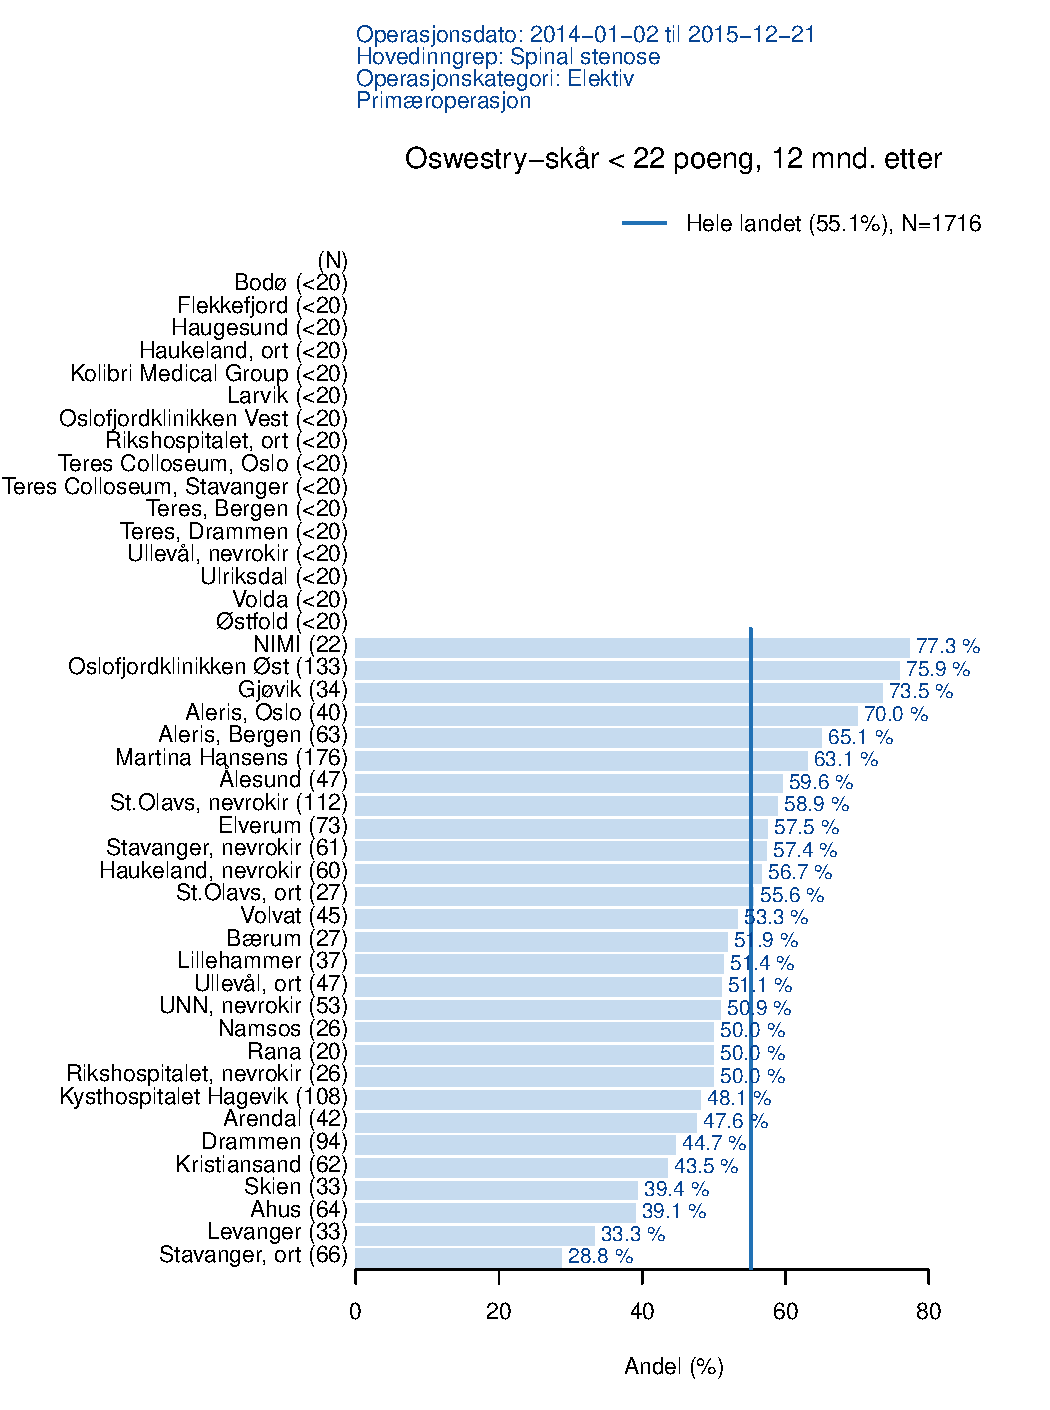
\includegraphics{Figurer/FigOsw22SS.pdf}}
\caption{\label{fig:Osw22SS}   Andel pasienter med ODI under 22 ett år
      etter spinal stenose operasjon. Pasienter operert i 2015 og 2016.}
\end{figure}


\clearpage

\subsection{Opplevd nytte av operasjon}
På spørreskjema etter operasjon blir pasientene bedt om å si hvor stor nytte de har hatt av operasjonen.
% De syv svaralternativene er angitt nedenfor og vår vitenskapelig baserte tolkinig er i parentes:
      % \begin{itemize}
% \item ''helt bra'' og ''mye bedre'' (Klart bedre)
% \item ''litt bedre'', ''ingen endring'' og ''litt verre'' (uendret) 
% \item ''mye verre'' og ''verre enn noen gang før'' (klar verre)
% \end{itemize}
Andelen som opplever at de har blitt helt bra eller mye bedre ett år etter operasjon har ligget stabilt siden 2011 og var 74\% for lumbalt prolaps og 60\% for spinal stenose opererte (2017) . Andelen  som angir at de er klart verre er henholdsvis har ligget stabilt rundt 3,0 \% for lumbalt prolaps og 5,5 \% spinal stenose opererte.
Et viktig fokusområde for NKR er å redusere andelen ryggopererte som får et dårlig operasjonsresultat.



      
      % \begin{figure}[h] 
% \begin{center}
% \scalebox{s2}{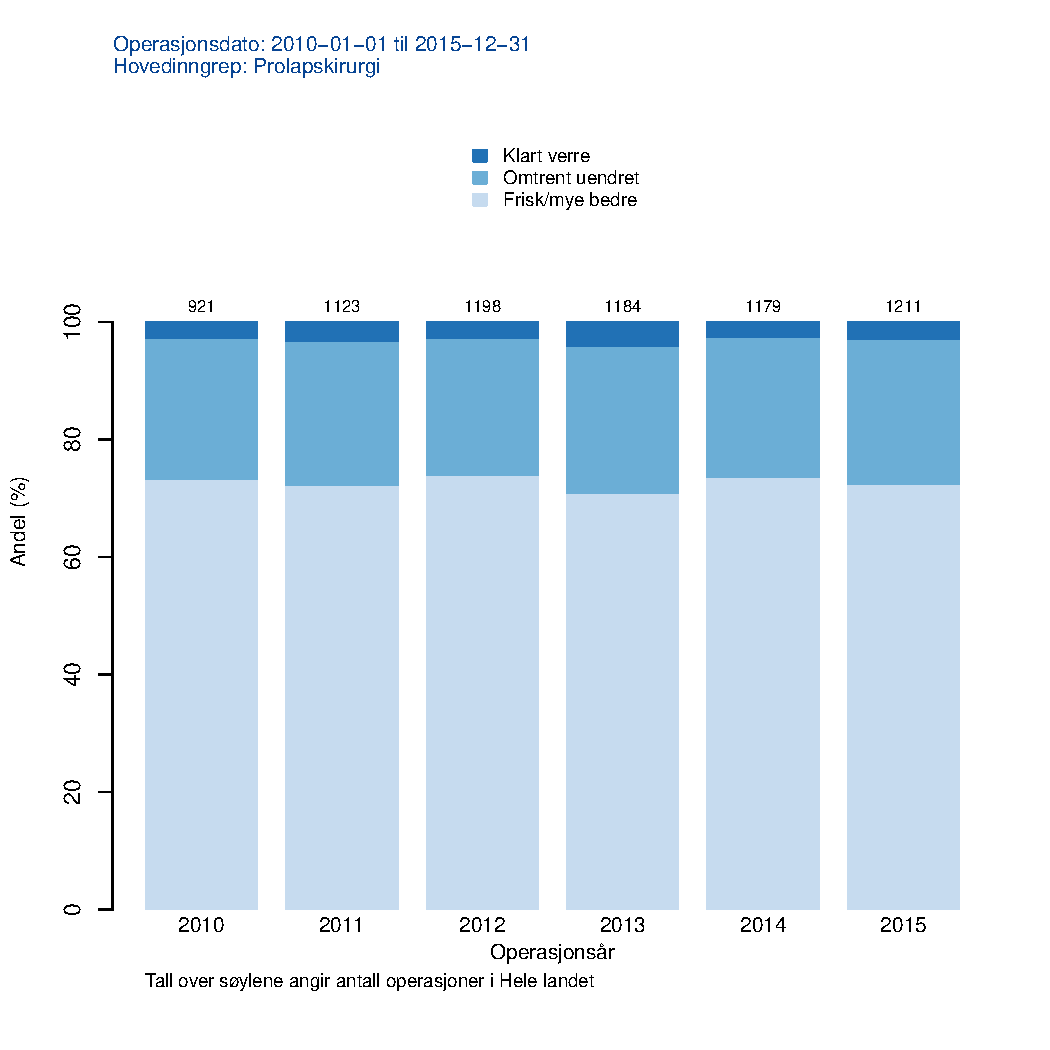
\includegraphics{Figurer/FigNyttePro.pdf}}
% \scalebox{s2}{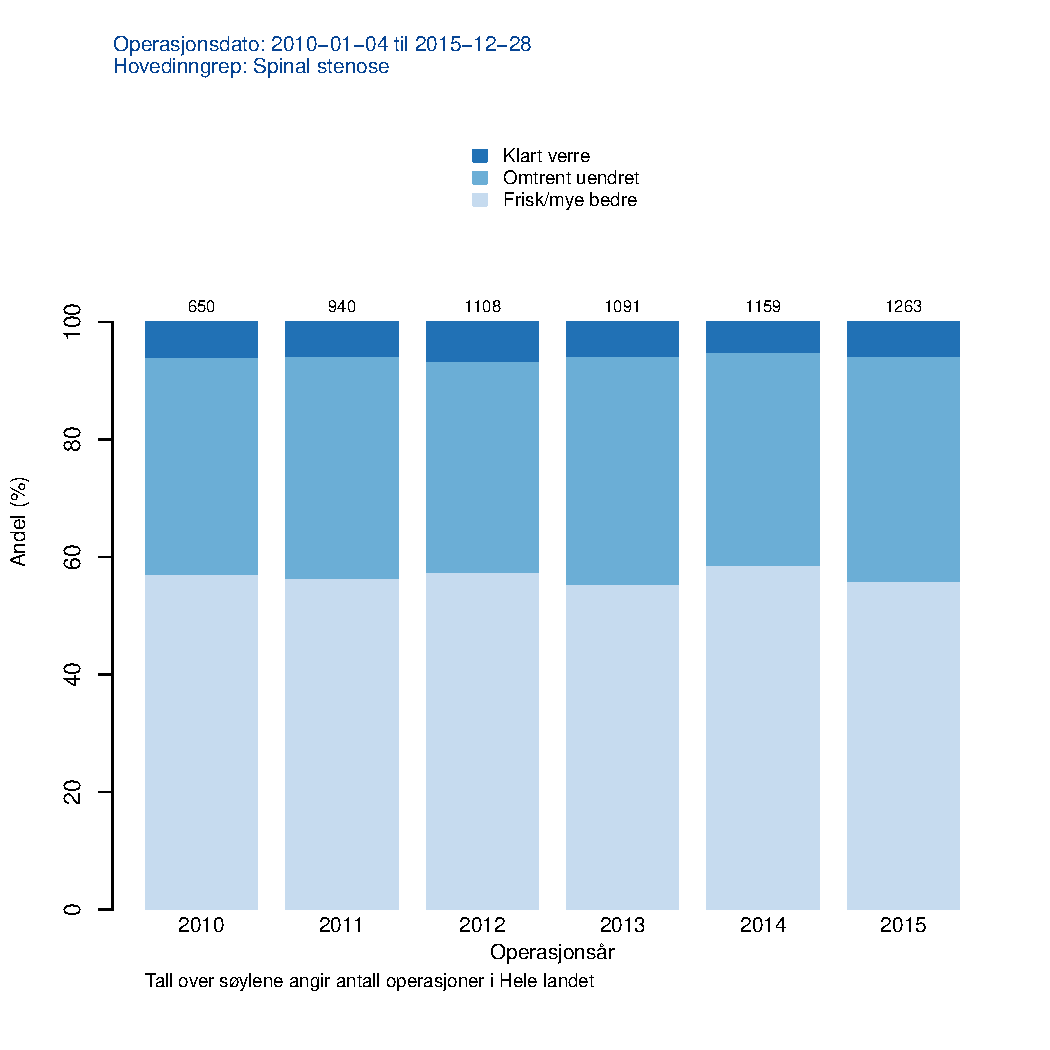
\includegraphics{Figurer/FigNytteSS.pdf}}
% \end{center}
% \caption{Spørsmål stilt 12 måneder etter operasjon til henholdsvis prolaps- og spinal stenosepasienter$:$ Hvilken nytte mener du at du har hatt av operasjonen?}
% \label{fig:Nytte}
% \end{figure}

\subsection{Pasienttilfredshet (PREM)}

% Figur \ref{fig:Fornoyd} viser hvor fornøyde pasientene var med behandlinga de fikk på sykehuset ktrtxt 
% etter operasjon fordelt på operasjonsår. Tallet øverst på søyla angir antall pasienter som har svart. 
På spørreskjemaet kan pasienten angi ett av 5 svaralternativer:
      \begin{itemize}
\item Fornøyd
\item Litt fornøyd
\item Hverken fornøyd eller misfornøyd
\item Litt misfornøyd
\item Misfornøyd
\end{itemize} 

 
Svarert på dette spørsmålet gjenspeiler et totalinntrykk og vil avhenge av en rekke andre faktorer enn selve den kirurgiske behandlingen. Andelen pasienter operert for lumbalt prolaps som ett år etter behandlinga er fornøyde med behandlingen de fikk på sykehuset  
ligger mellom 78 \% og 81 \% 
      for pasienter operert i perioden. 
%      startAar-rappAar. 
Tilsvarende ligger andel for lumbal spinal stenose ligger mellom 73 \% 
og 77 \%
Lumbal spinal stenose opererte gjennomgående var litt mindre fornøyd med behandlingen de fikk på sykehuset sammenliknet med prolapspasientene.





      
      % \begin{figure}[h] 
% \begin{center}
% \scalebox{s2}{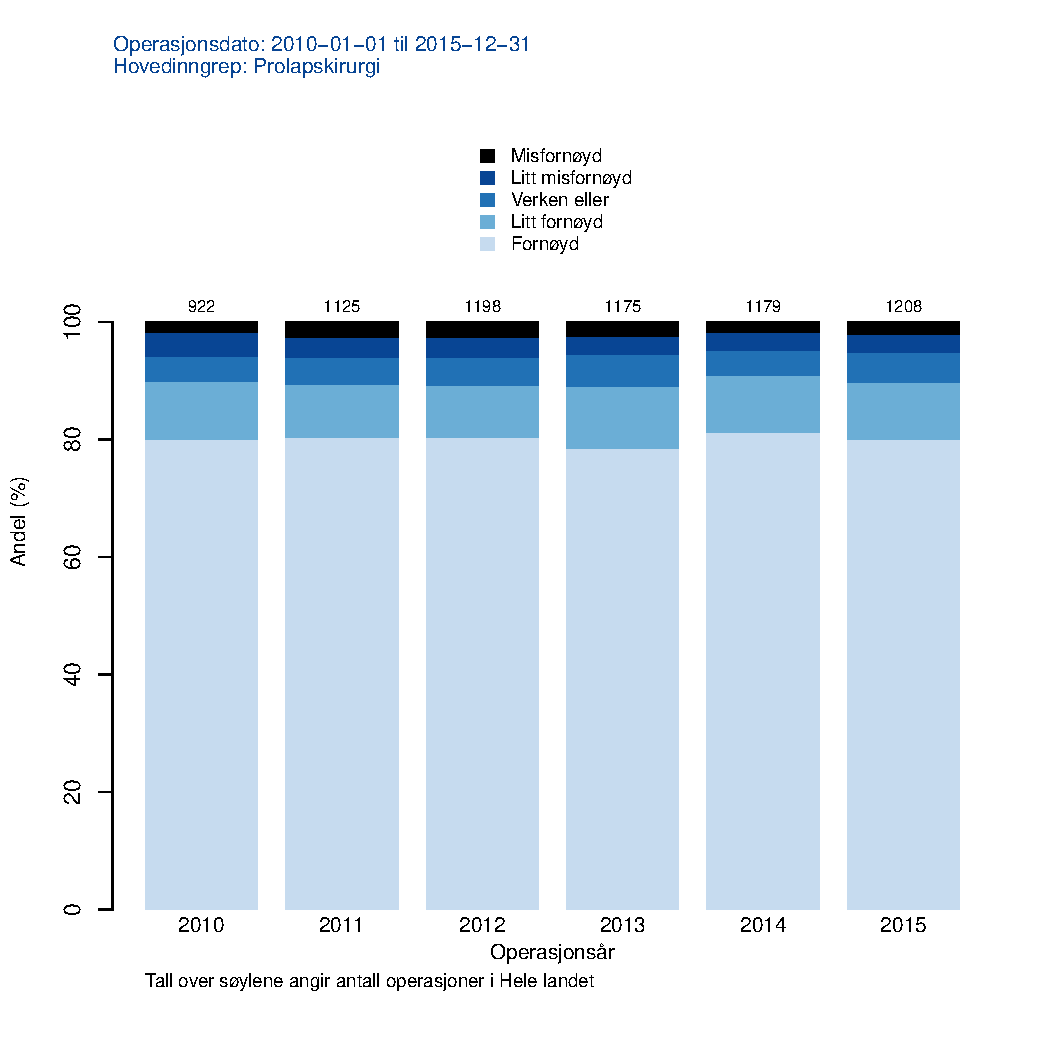
\includegraphics{Figurer/FigFornoydPro.pdf}}
% \scalebox{s2}{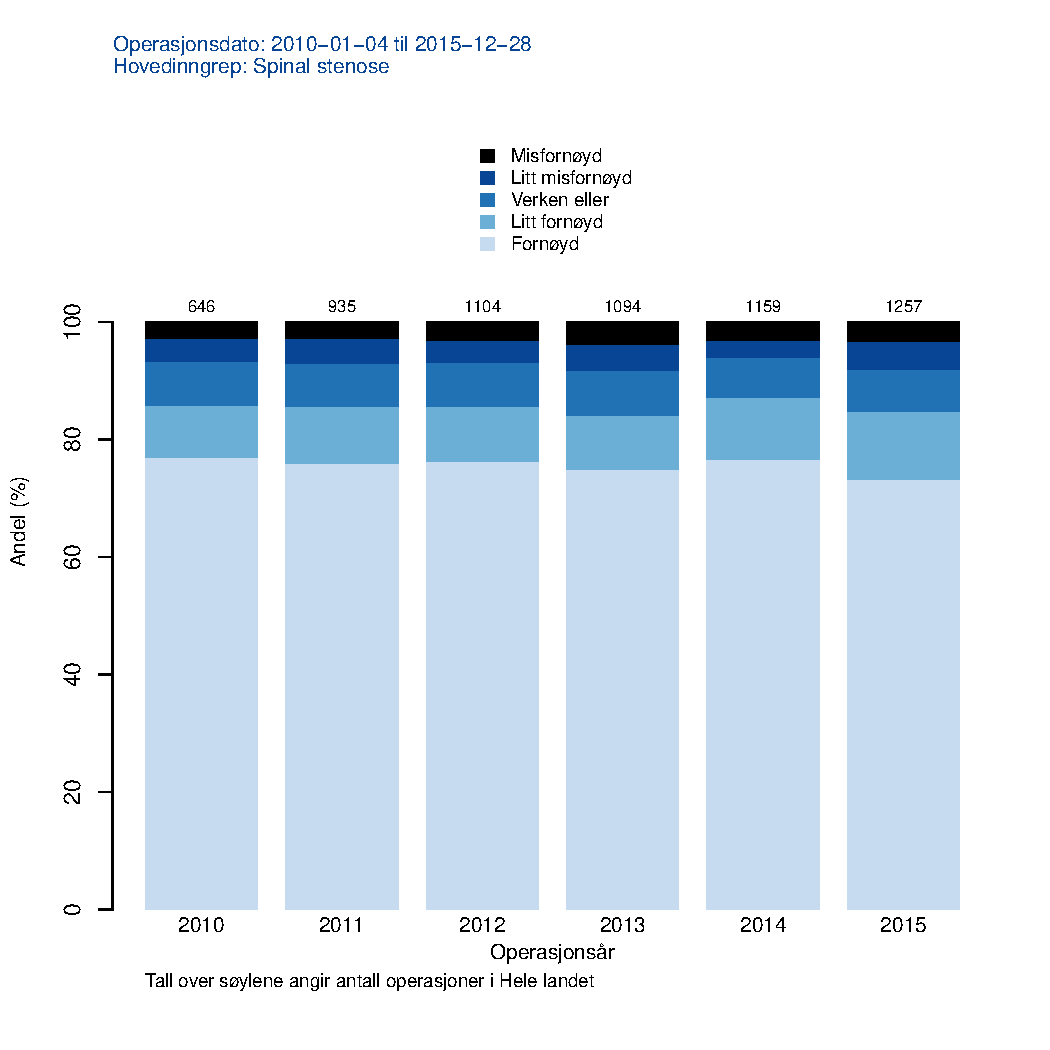
\includegraphics{Figurer/FigFornoydSS.pdf}}
% \end{center}
% \caption{Spørsmål stilt 12 måneder etter operasjon: Hvor fornøyd er du med behandlinga du har fått på sykehuset? til henholdsvis prolaps- og spinal stenosepasienter}
% \label{fig:Fornoyd}
% \end{figure}

\begin{figure}[h] 
\scalebox{0.7}{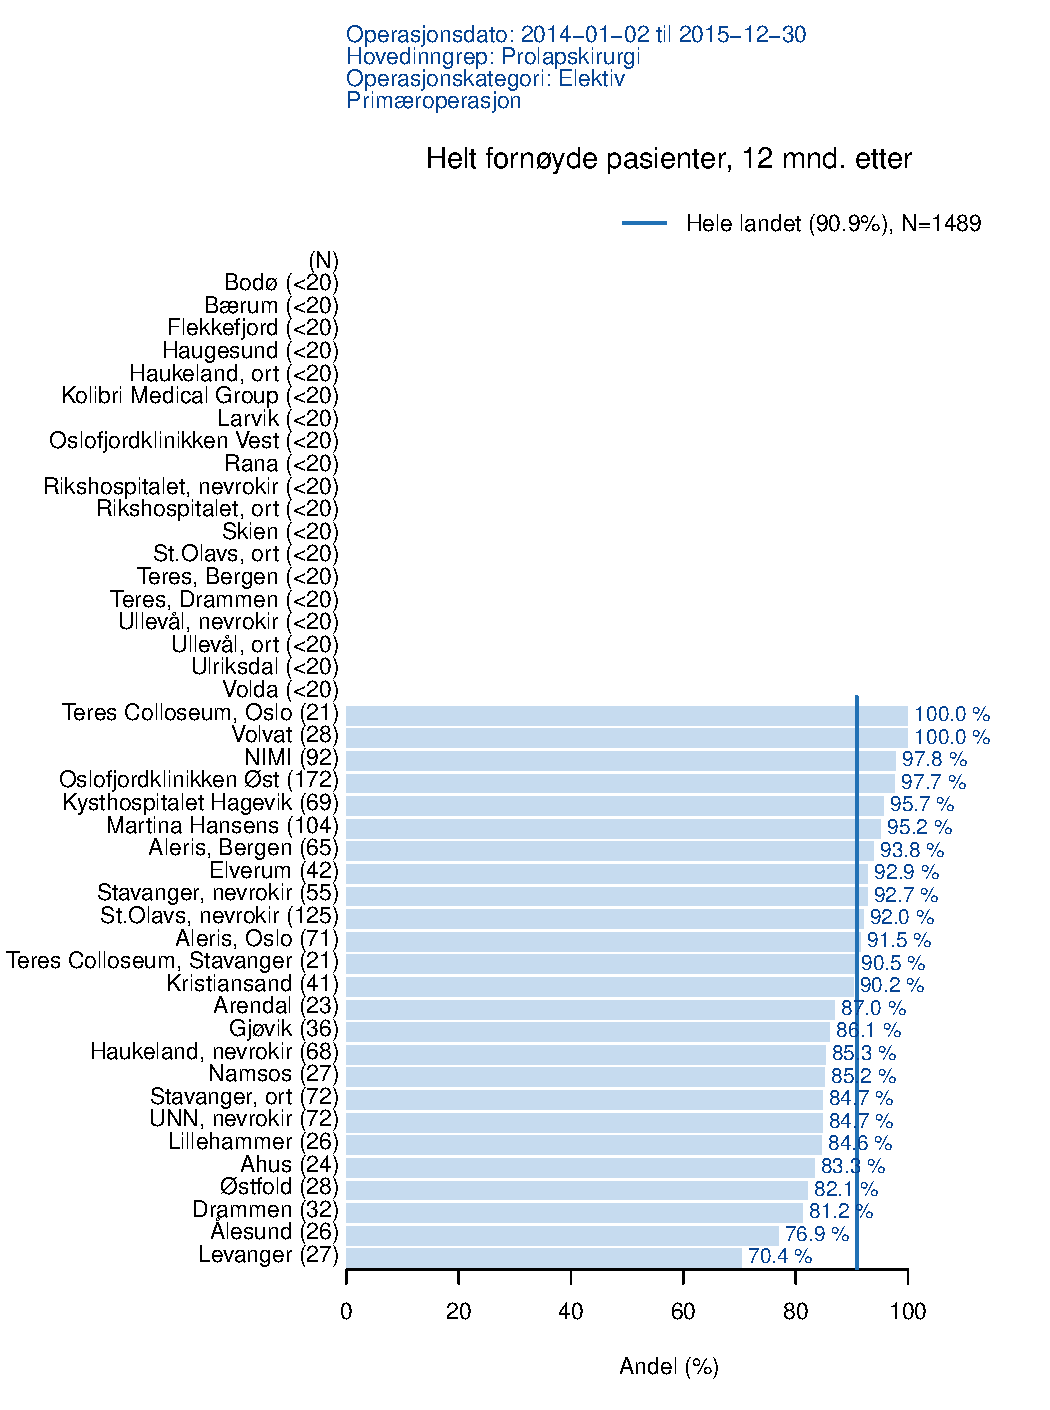
\includegraphics{Figurer/FigFornoydAvdPro.pdf}}
\caption{Andel pasienter operert for lumbalt prolaps i 2015 og 2016, som ett år etter er helt fornøyde med behandlinga de har fått på sykehuset}
\label{fig:FornoydAvdPro}
\end{figure}

\begin{figure}[h] 
\scalebox{0.7}{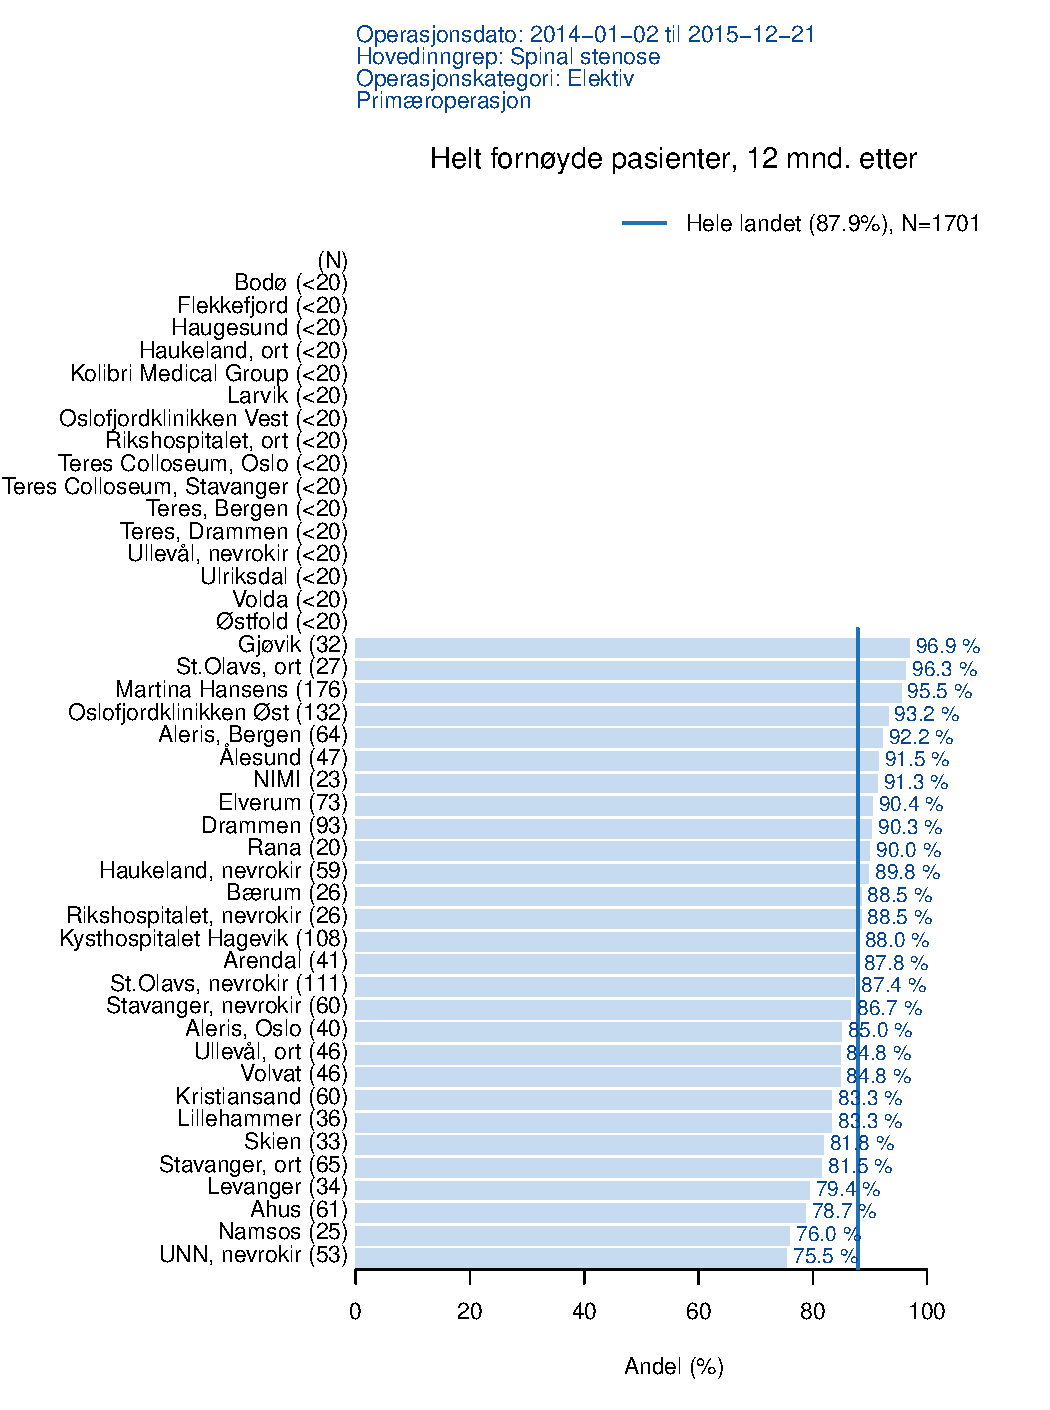
\includegraphics{Figurer/FigFornoydAvdSS.pdf}}
\caption{Andel pasienter opertert for lumbal spinal stenose i 2015 og 2016, som etter ett år er helt fornøyde med behandlinga de har fått på sykehuset}
\label{fig:FornoydAvdSS}
\end{figure}

\clearpage




      
      % Gjennomsnittlig liggetid på sykehus i forbindelse med prolapsoperasjon har gått ned med 
% NedgLiggetidPro døgn fra 2010 til rappAar.



\subsection{Kvalitetsindikatorer}
Det er viktig å merke seg at "indikator"  betyr en \textbf{mulig} sammenheng 
med kvalitet. Om indikatoren peker på et område som kan forbedres, må vurderes på det enkelte sykehus.

\subsubsection{Degenerativ rygg}



%\subsubsection{Sykehusvise resultater}


      
      Resultatene nedenfor gjelder planlagt, første gangs operasjon for lumbal spinal stenose og prolaps.
Kun avdelinger med mer enn 10 evt. 20 (avhenger av type resultat) registrerte operasjoner i er med i
analysen.
Grunnen til at reoperasjon og øyeblikkelig hjelp (ø-hjelp)
er filtrert bort er at andel slike inngrep er ulikt fordelt mellom sykehusene. 
      ''Suksess'' er her definert som mer enn 20 poengs forbedring av ODI. 
Hos pasienter med lumbalt prolaps som ikke har vært operert i ryggen tidligere er 
suksessraten 63.4 \% mot 54.8 \%. Hos prolapspasienter operert som ø-hjelp er andelen med betydelig forbedring 
(suksessrate)  78.7 \%, mot 57 \% av de som blir 
operert planlagt (elektivt). Dersom man har vært operert mer enn 2 ganger tidligere i
ryggen faller suksessraten fra  for lumbal spinal stenoseopererte betydelig (10\%). Langt færre pasienter i spinal stenosegruppen opereres som øyeblikkelig hjelp; 0.6 \%.  

Sykehus som får henvist få pasienter som ø-hjelp og
mange til reoperasjon vil dermed få dårligere resultater. 

 



For degenerativ rygg har fagrådet til NKR har valgt ut de kvalitetsindikatorerne som er angitt i tabell \ref{tab:KvalInd}
i kapittel \ref{sec:regspe}. 

\subsubsection{Dekningsgrad (Strukturmål)}
Høy dekningsgrad er en forutsetning for å kunne drive kvalitetssikring av egen virksomhet. Dekningsgraden gjenspeiler de ulike sykehusenes evne til og interesse for å evaluere sine egne resultater.
Lena: sett inn figur med fagekoder.

\clearpage

\subsubsection{Symptomvarighet for operasjon (Prosessmål)} 

Andelen pasienter som har hatt beinsmerter mer enn ett år på
operasjonstidspunktet var uendret fra 2011 til 2017 (47\%). 
I nasjonale retningslinjer (2007) er det anbefalt å operere pasienter for lumbalt prolaps før
beinsmertene har vart for lenge, helst innen ett år. Derfor bør denne
pasientgruppen håndteres raskt og effektivt når beslutning om operasjon er tatt og
ikke-kirurgisk behandling har vært forsøkt. Data fra NKR og nyere forskning viser at
pasienter som opereres for prolaps og har hatt beinsmerter mer enn ett år har
dårligere prognose. 
Det er stor variasjon i varighet av beinsmerter hos pasienter som blir
operert ved ulike sykehus. Det har sannsynligvis sammenheng med ventetid for
utredning og operasjon og tilgjengelig operasjonskapasitet i forhold til etterspørsel.
Lena: sett inn figur med fagekoder, dvs. varighet av bensmerter før operasjon.

Tabellen  \ref{tab:Utstr} viser fordeling av hvor lenge pasientene har hatt utstrålende smerter. 
Figurene \ref{fig:VarighSmerteUtstrAvdPro} og \ref{fig:VarighSmerteUtstrAvdSS} viser hvor stor andel av henholdsvis prolaps- og spinal stenosepasienter som har hatt ustrålende smerter i mer enn ett år ved hvert sykehus.

Det er bekymringsfult liten reduksjon i symptomvarighet før kirurgi fra år til år, spesielt for gruppen som ble opereret for lumbalt prolaps.


% latex table generated in R 3.5.0 by xtable 1.8-2 package
% Wed Sep 26 12:17:09 2018
\begin{table}[ht]
\centering
\begin{tabular}{lr}
  \hline
 & Andeler \\ 
  \hline
Ingen utstrålende smerter & 3\% \\ 
  $<$ 3 mnd & 12.4\% \\ 
  3 - 12 mnd & 35.1\% \\ 
  1 - 2 år & 18.7\% \\ 
  $>$ 2 år & 25.8\% \\ 
  Ikke besvart & 5.1\% \\ 
   \hline
\end{tabular}
\caption{Varighet av nåværende utstrålende smerter} 
\label{tab:Utstr}
\end{table}

      
      




 


\begin{figure}[h] 
\scalebox{0.7}{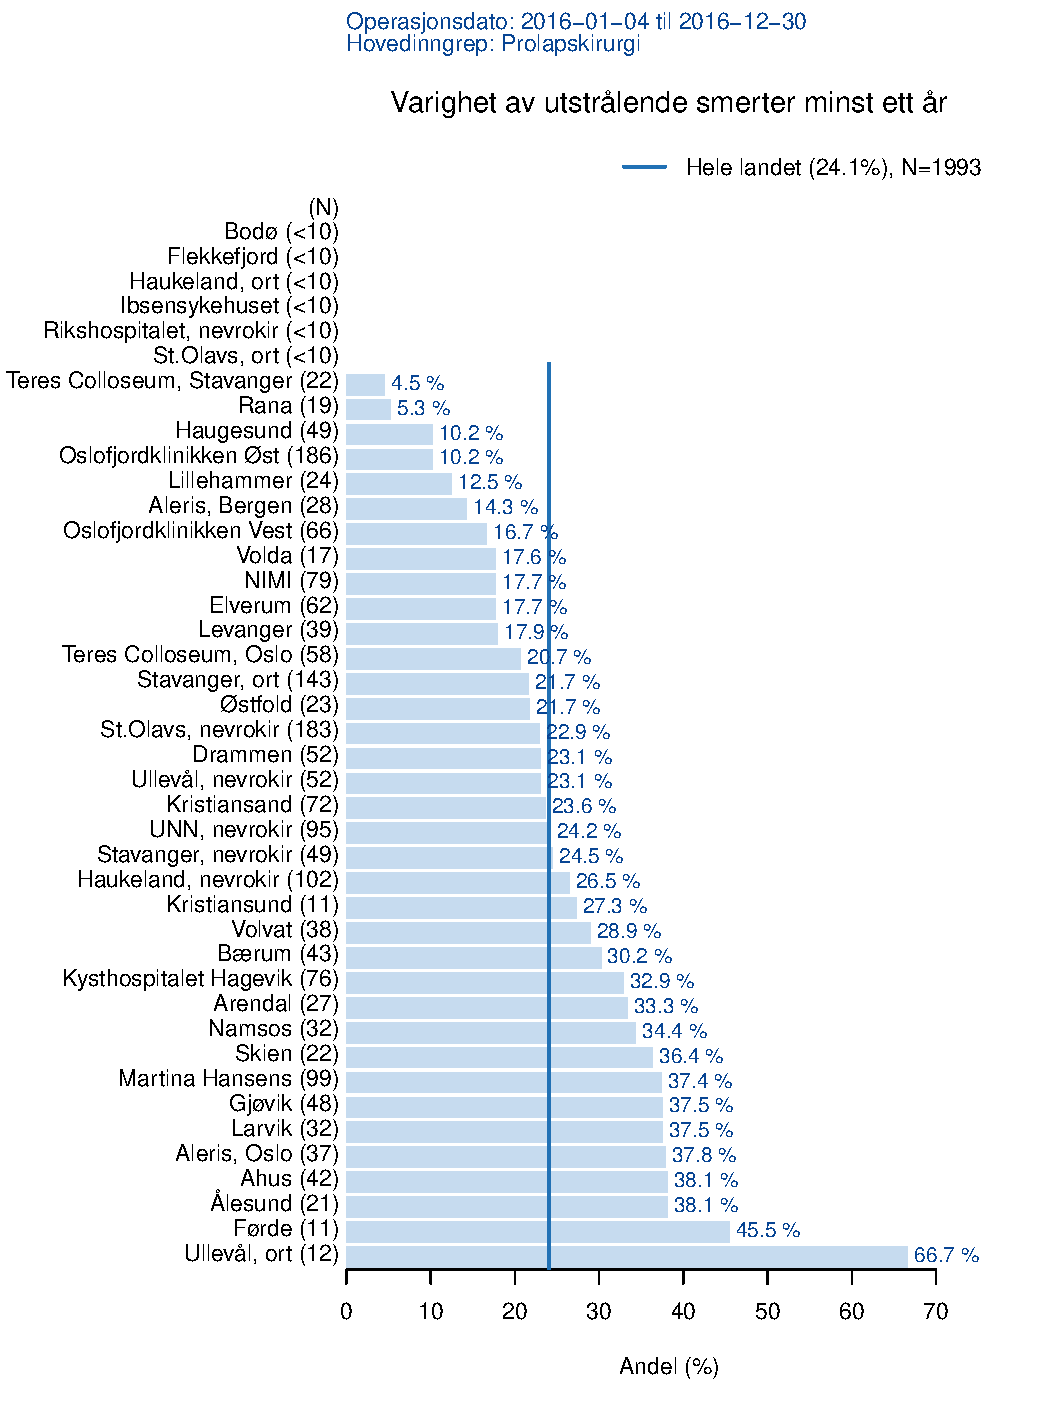
\includegraphics{Figurer/VarighUtstrAvdPro.pdf}}
\caption{Lumbale prolapspasienter som har hatt utstrålende smerter i mer enn ett år før operasjonen.}
\label{fig:VarighSmerteUtstrAvdPro}
\end{figure}

\begin{figure}[h] 
\scalebox{0.7}{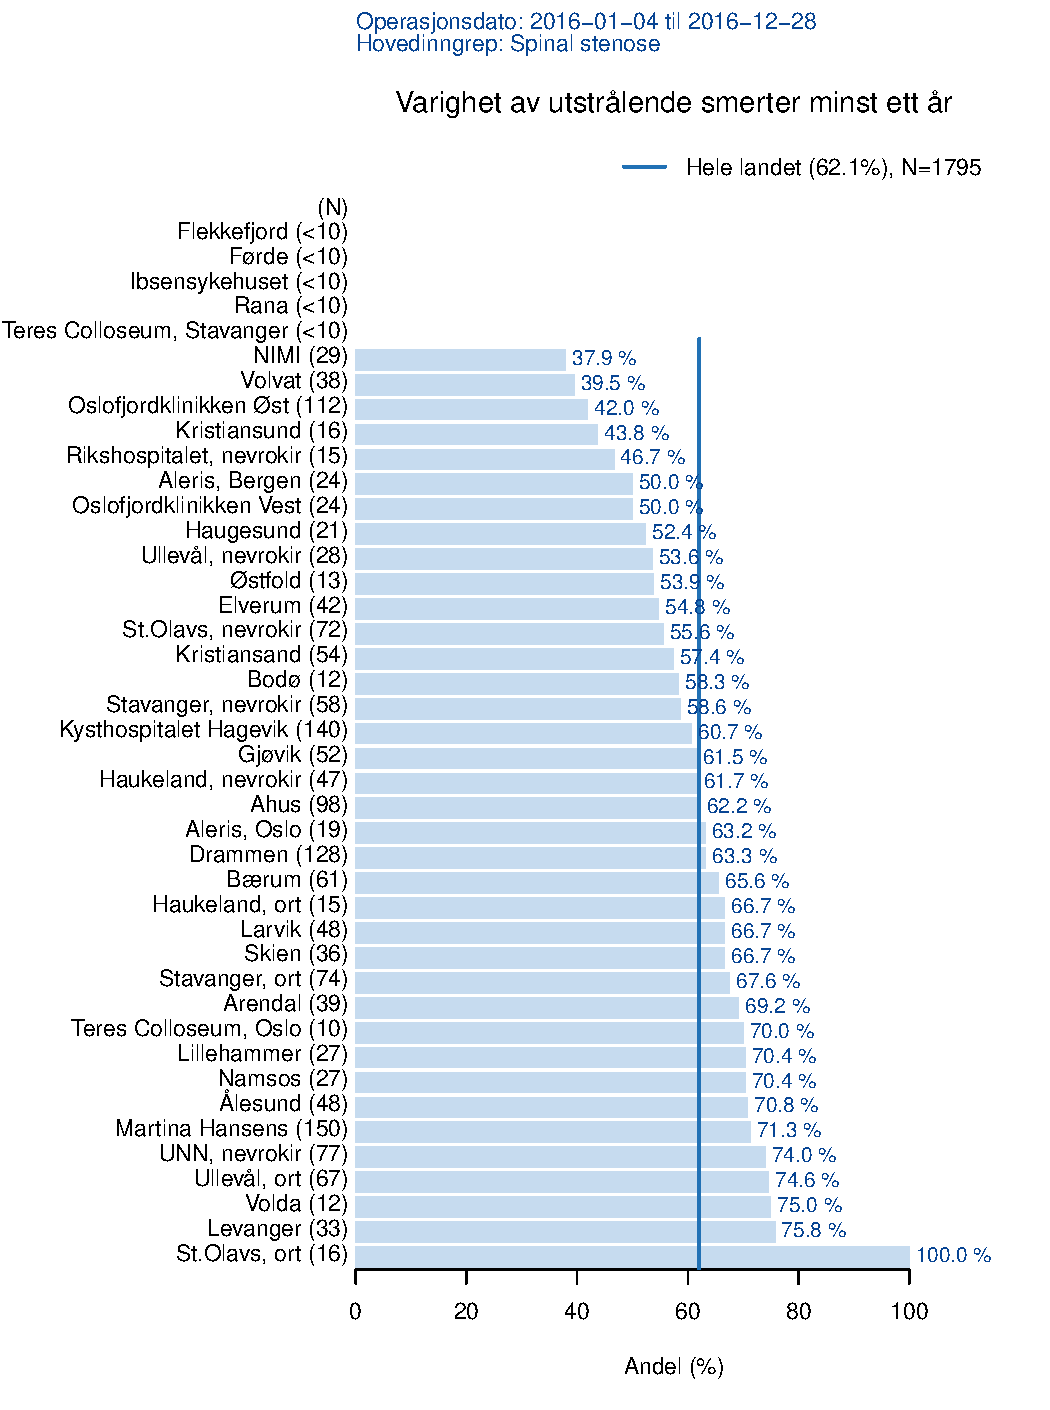
\includegraphics{Figurer/VarighUtstrAvdSS.pdf}}
\caption{Lumbal spinal stenosepasienter som har hatt utstrålende smerter i mer enn ett år før operasjonen.}
\label{fig:VarighSmerteUtstrAvdSS}
\end{figure}

Figur \ref{fig:VarighSmerteUtstrTid} viser utvikling over tid for andel pasienter med lang symptomvarighet. 

\begin{figure}[h] 
\center{
      \scalebox{0.55}{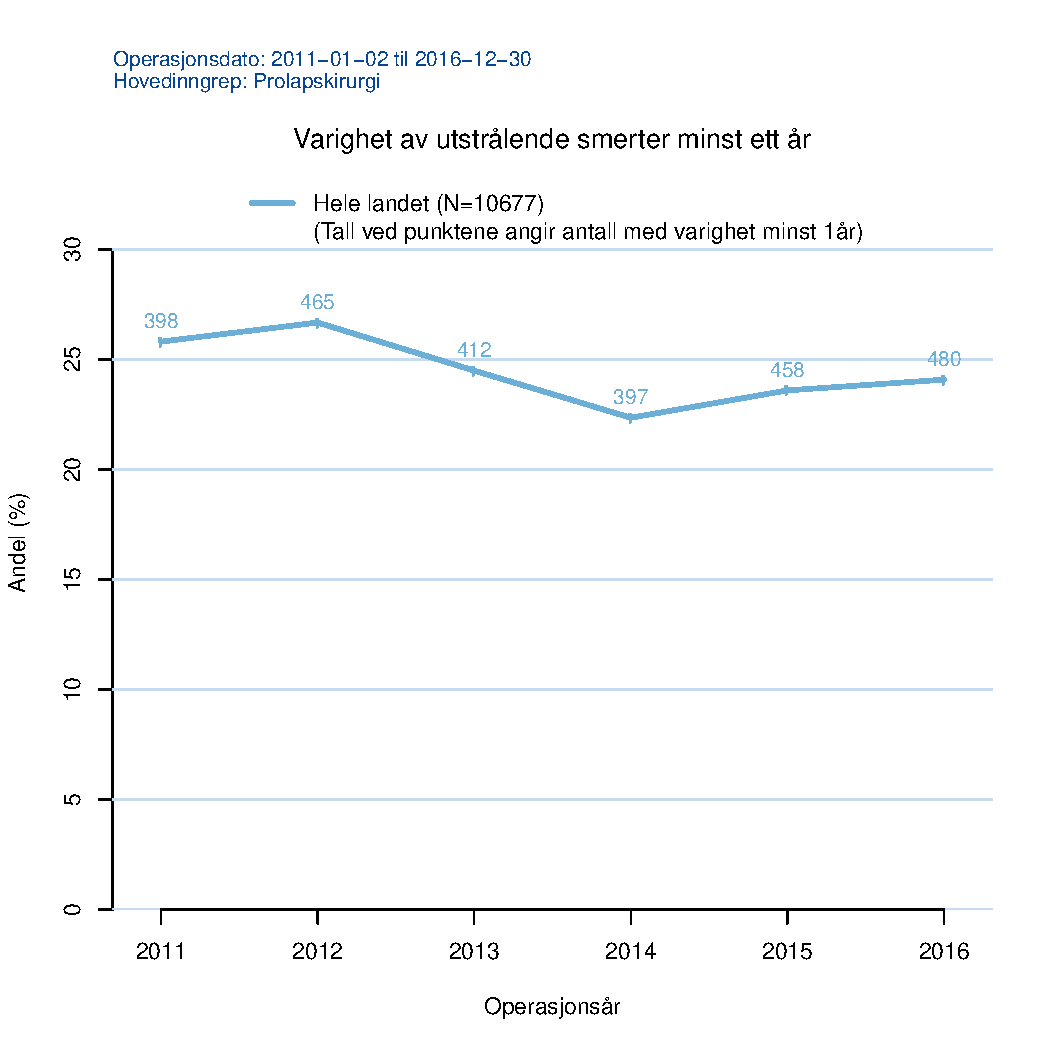
\includegraphics{Figurer/VarighUtstrTidPro.pdf}}
      \scalebox{0.55}{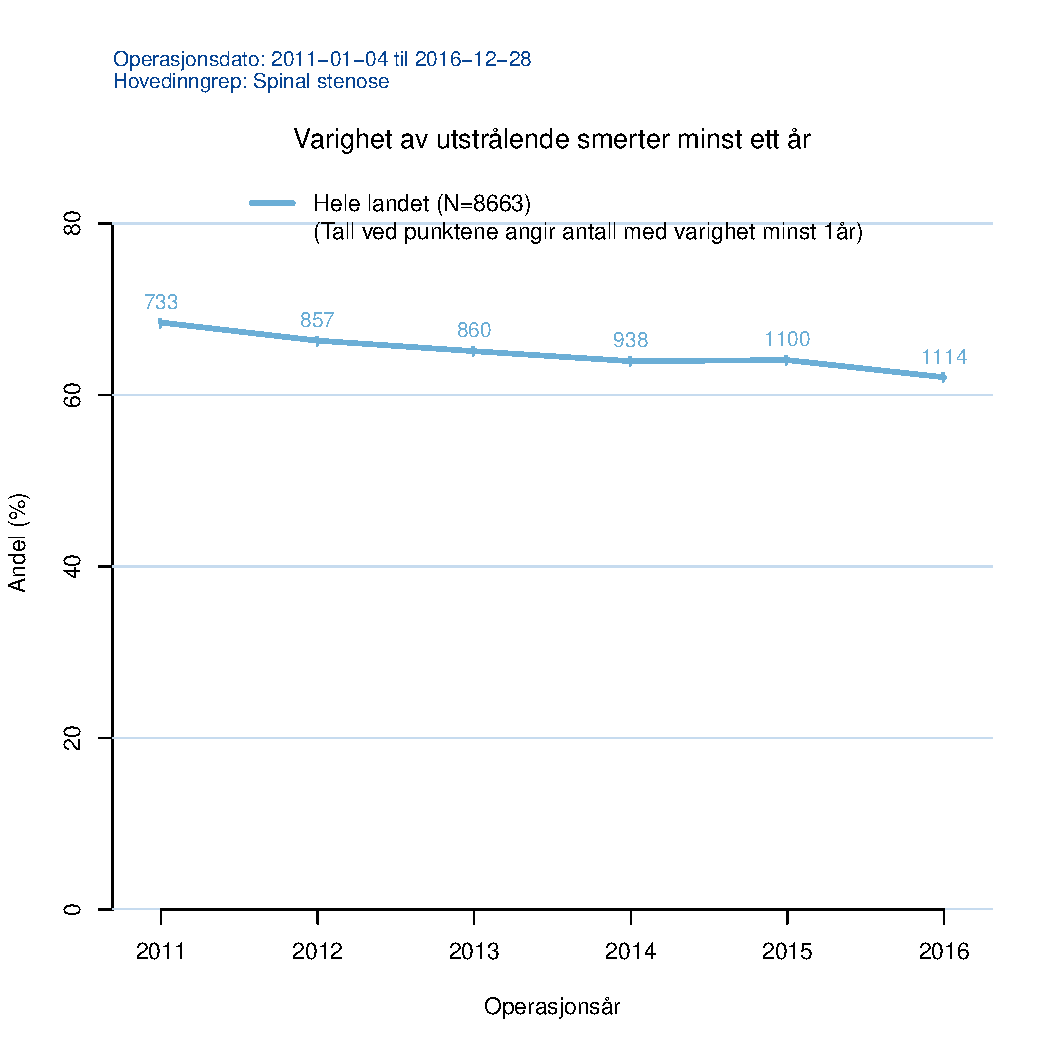
\includegraphics{Figurer/VarighUtstrTidSS.pdf}}} 
\caption{Prolaps- og Spinal stenosepasienter som har utstrålende smerter i mer enn ett år før operasjonen, utvikling over tid.}
\label{fig:VarighSmerteUtstrTid}
\end{figure}


%Lena: kun utstrålende smerter.

%\begin{figure}[h] 
%\scalebox{s1}{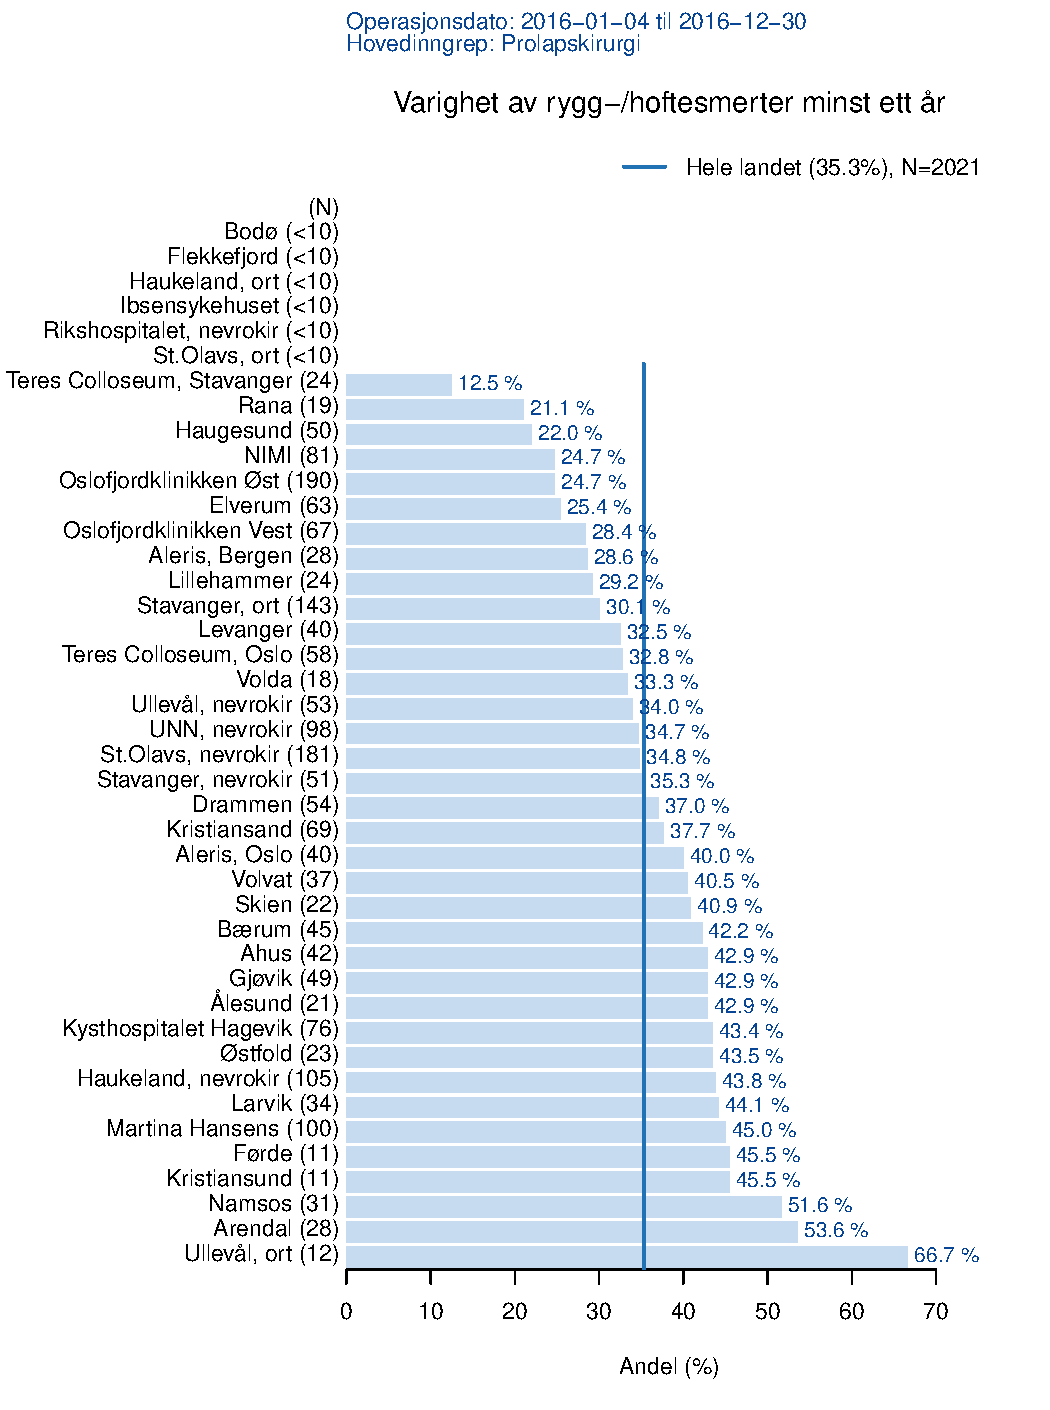
\includegraphics{Figurer/VarighRyggHofAvdPro.pdf}}
%\caption{Prolapspasienter som har hatt smerter i rygg-/hofte
      %i mer enn ett år før operasjonen.}
%\label{fig:VarighSmerteRyggAvdPro}
%\end{figure}

%\begin{figure}[h] 
%\scalebox{s1}{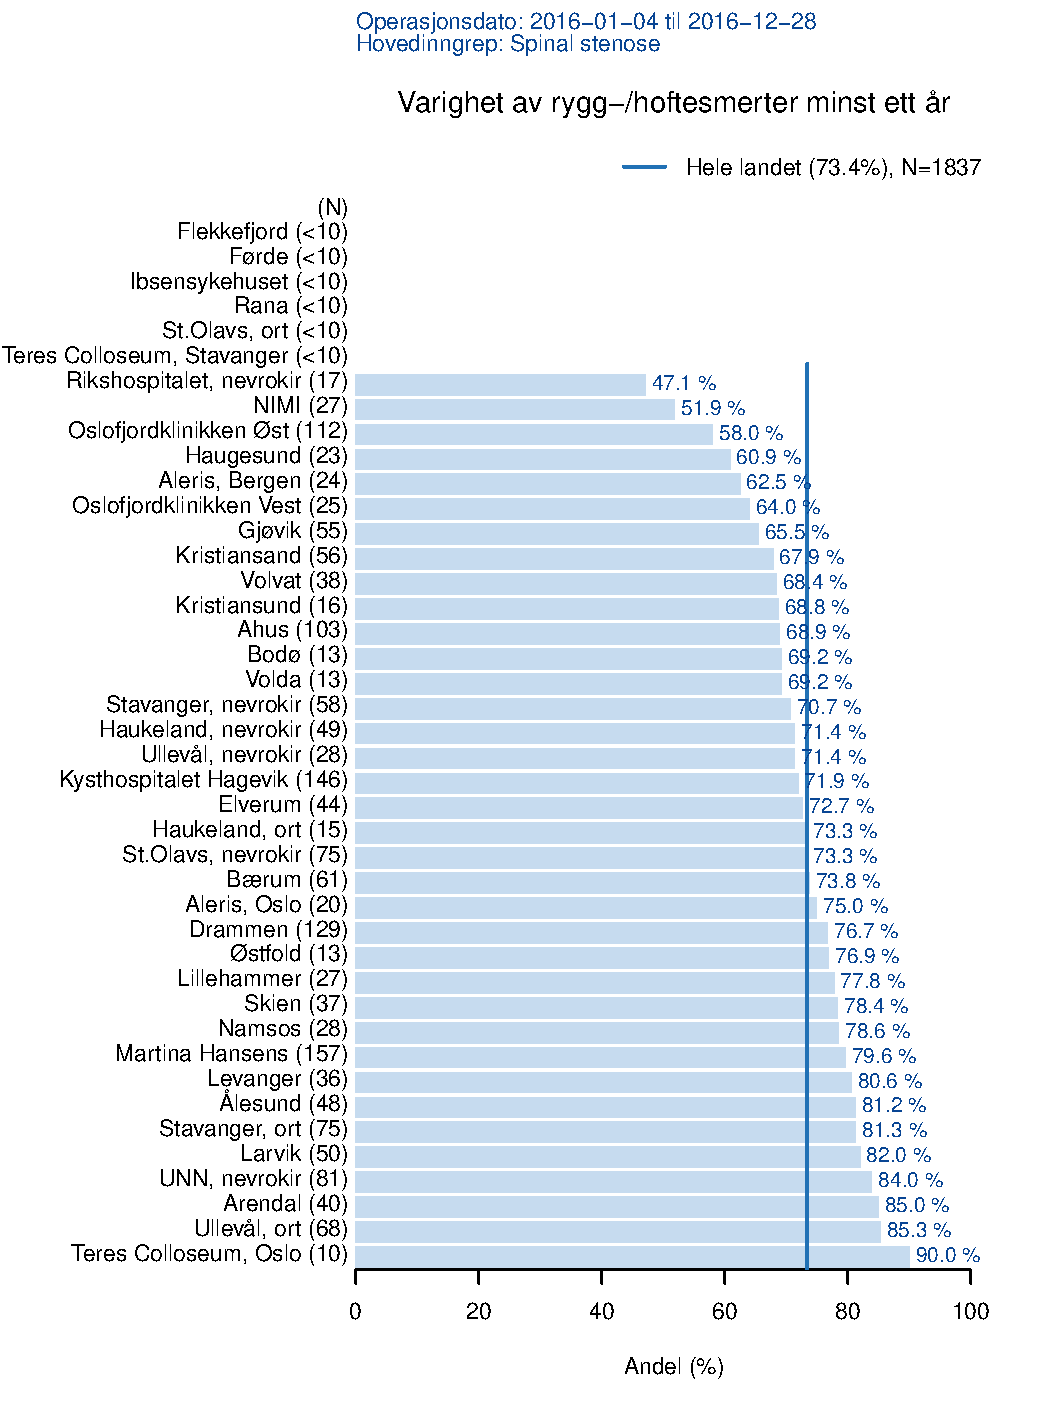
\includegraphics{Figurer/VarighRyggHofAvdSS.pdf}}
%\caption{Spinal stenosepasienter som har hatt smerter i rygg-/hofte
      %i mer enn ett år før operasjonen.}
%\label{fig:VarighSmerteRyggAvdSS}
%\end{figure}
									


 \subsubsection{Lite symptomer før operasjon (Prosessmål)}     
      Pasienter som har mye plager, vil kunne forvente størst nytte av ryggoperasjon,
mens de som har lite plager vil ha mindre potensial for forbedring og større risiko
for forverring. Gevinst av kirurgi henger derfor sammen med hvor streng
indikasjonsstillingen («inngangsbilletten» til kirurgi) har vært. Figur \ref{fig:BeinsmEndrPre} viser denne
sammenhengen tydelig. Det er verdt å merke seg er at hvis pasienten har lite smerter før
operasjon (bensmerter under eller lik 3 på den horisontale smerteskalaen), er det stor
sjanse for at pasienten faktisk blir verre  etter
operasjon (mindre enn 0 på den vertikale skalaen). \\

\begin{figure}[ht]
\scalebox{0.7}{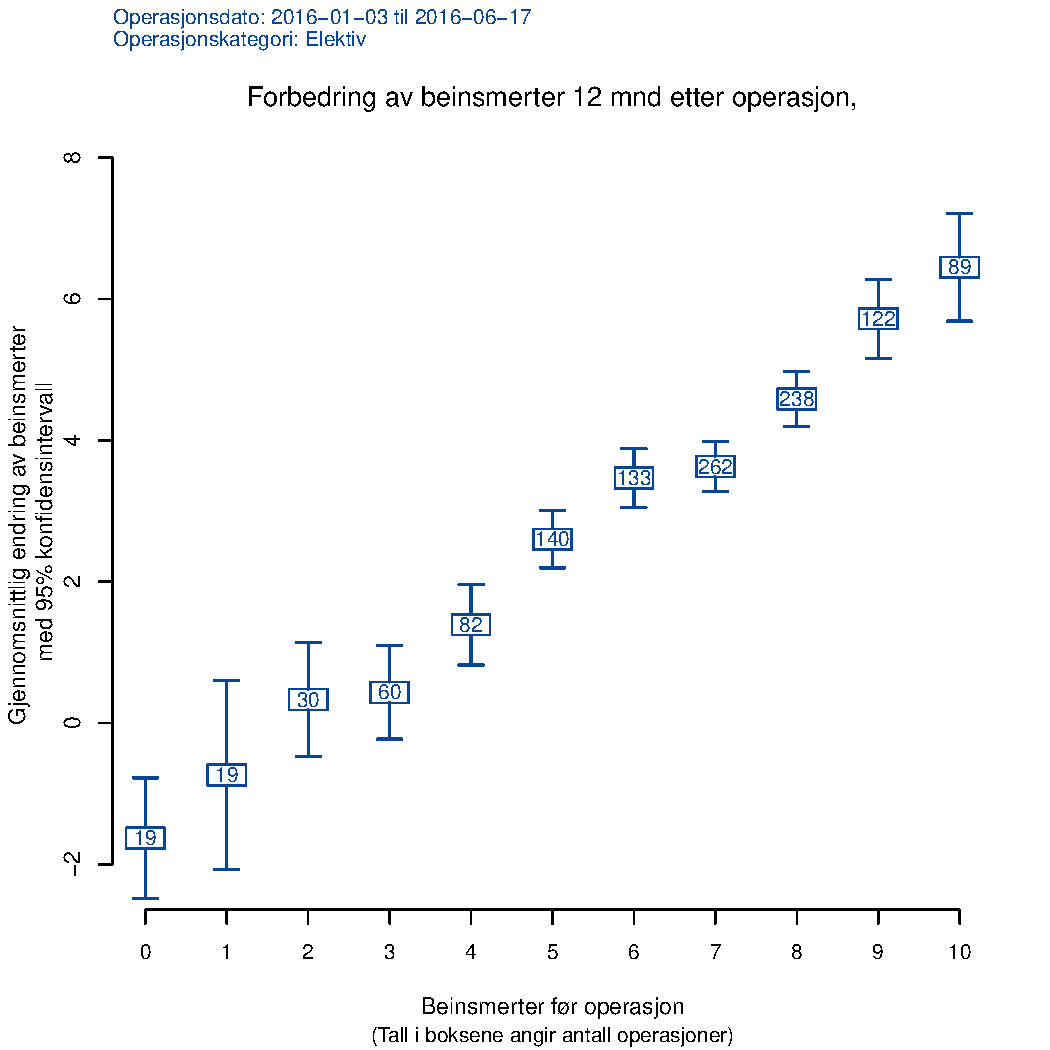
\includegraphics{Figurer/FigBeinsmEndrPre.pdf}}
\caption{\label{fig:BeinsmEndrPre}  Sammenheng mellom intensitet av bensmerte før operasjon og
      forbedring etter operasjon. Skala for bensmerter går fra 0 til 10, hvor 0 betegner
      ingen og 10 verst tenkelige smerte før operasjon (horisontal akse). Negativ endring
      av bensmerten (vertikal akse) tilsvarer forverring, 0 betyr uendret smerte etter
      operasjon.}
\end{figure}

\clearpage

Figur \ref{fig:BeinsmLavPre} viser at det er stor variasjon i hvor stor grad sykehusene opererer
pasienter med lumbalt prolaps og lite beinsmerter . Pasienter med lammelse (parese) er tatt
ut av analysen, da de ofte må opereres uansett grad av smerte.




\begin{figure}[ht]
\scalebox{0.7}{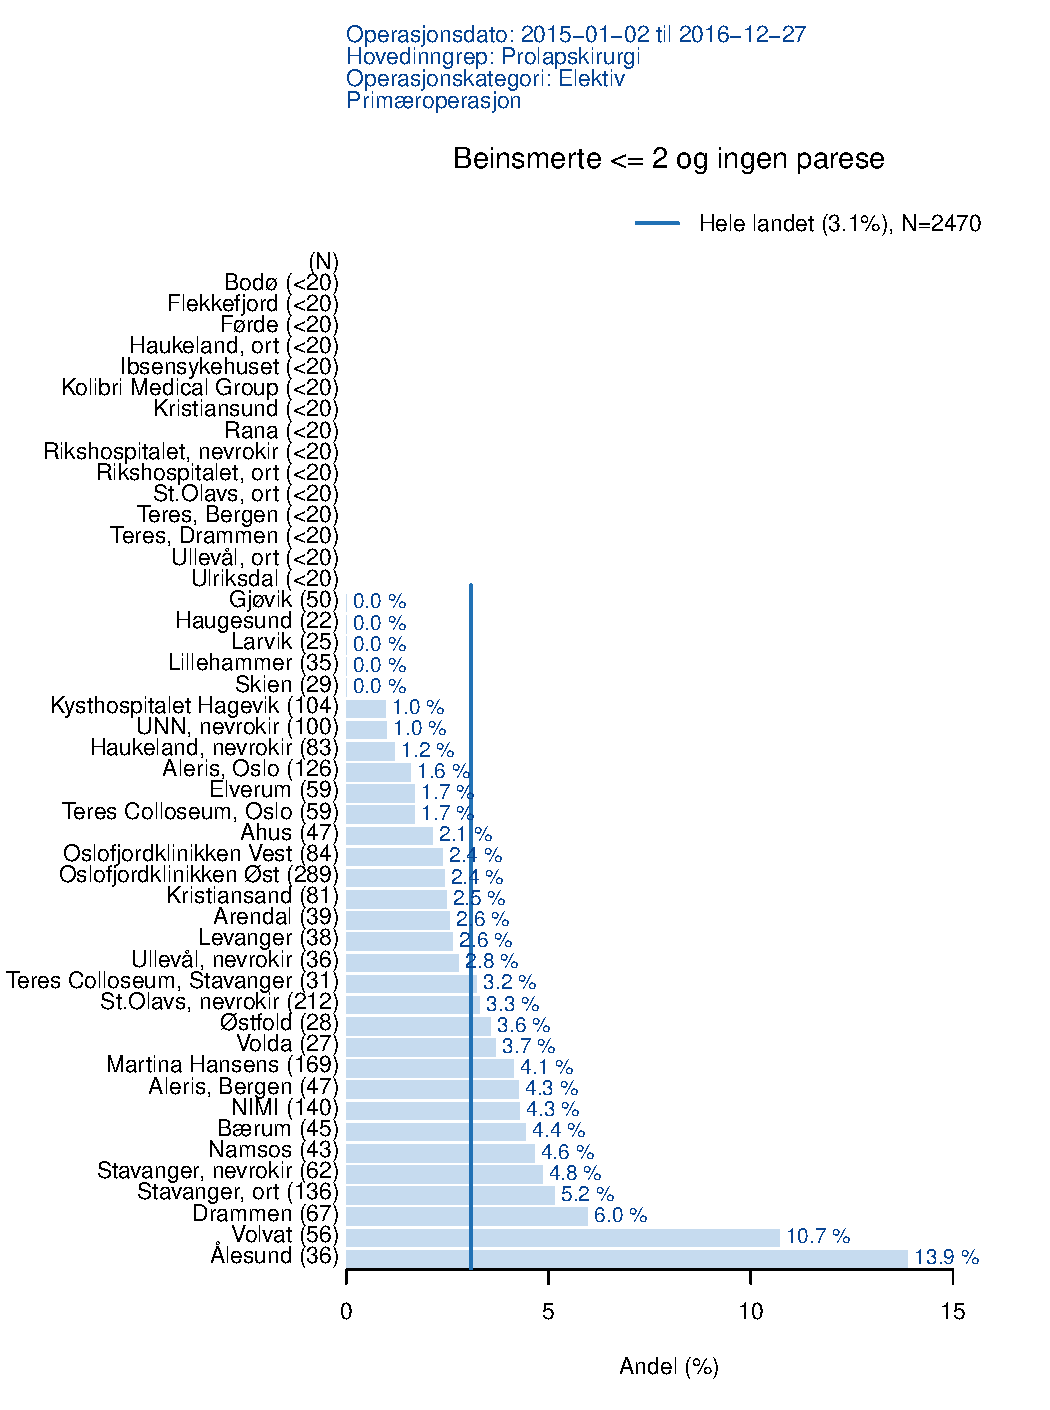
\includegraphics{Figurer/FigBeinsmLavPre.pdf}}
\caption{\label{fig:BeinsmLavPre}  Andel pasienter med lite beinsmerter ($\leq 3$) operert for prolaps.}
\end{figure}






\subsubsection{Sårinfeksjon (Resultatmål)}




\textbf{I. Sårinfeksjon.}

Årsakene til sårinfeksjon er komplekse. NKR viste for mange år siden at dette har god forbyggende effekt. For lumbale prolaps operasjoner har
andel sårinfeksjoner (pasientrapportert) har blitt noe redusert fram til 2011, samtidig med at forbyggende antibiotikabehandling økte sterkt. I dag får 99\% antibiotika ved kirurgi for lumbalt prolaps og spinal stenose. Siden 2011 har andelen sårinfeksjoner ligget stabilt rundt 2 \% for prolapsopererte og rundt 3 \% for spinal stenose opererte.
Figurene \ref{fig:KpInfAvdPro} og \ref{fig:KpInfAvdSS} viser andel pasienter som fikk sårinfeksjon ved hver avdeling i årene 2016 og 2017.

      


%\begin{figure}[ht]
%      \centering \scalebox{s2}{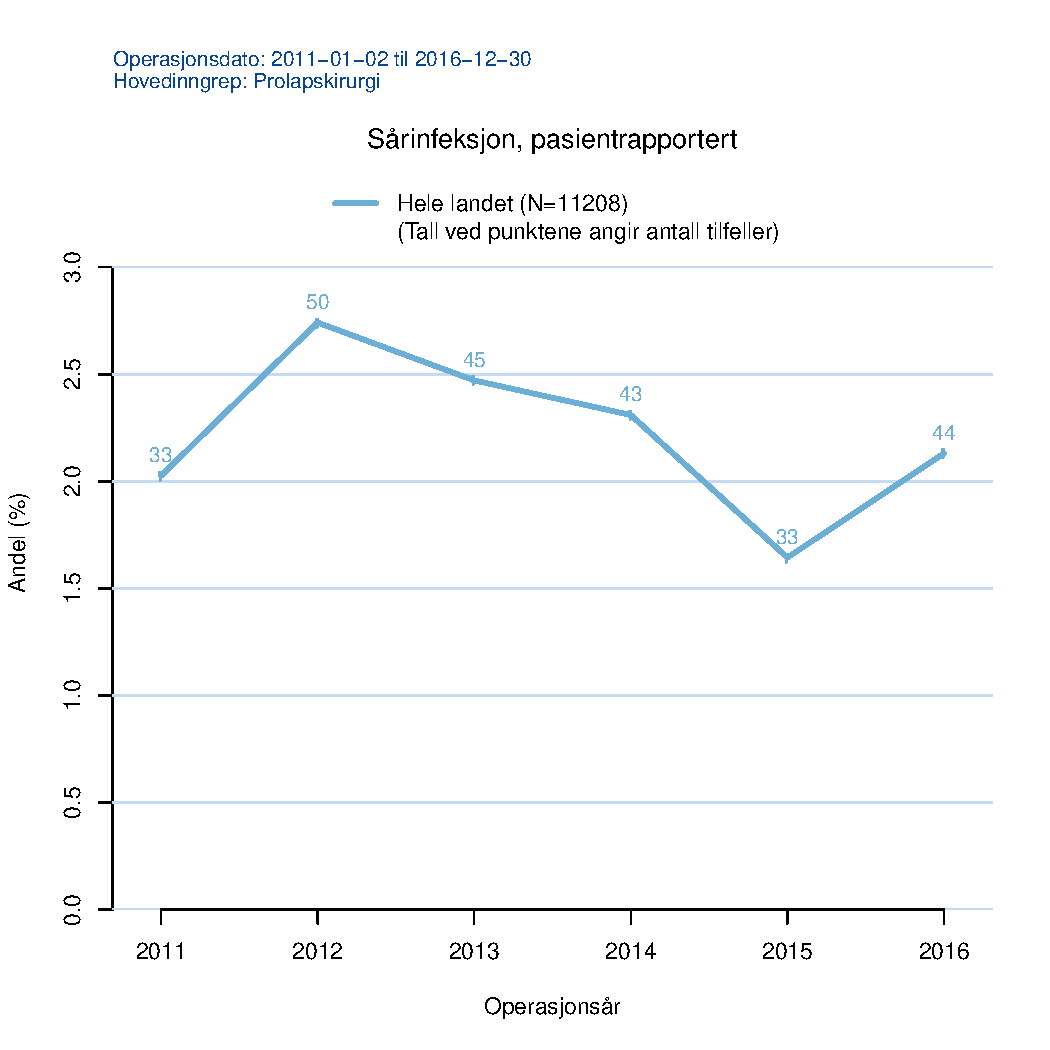
\includegraphics{Figurer/FigKpInf3MndTidPro.pdf}}
%      \centering \scalebox{s2}{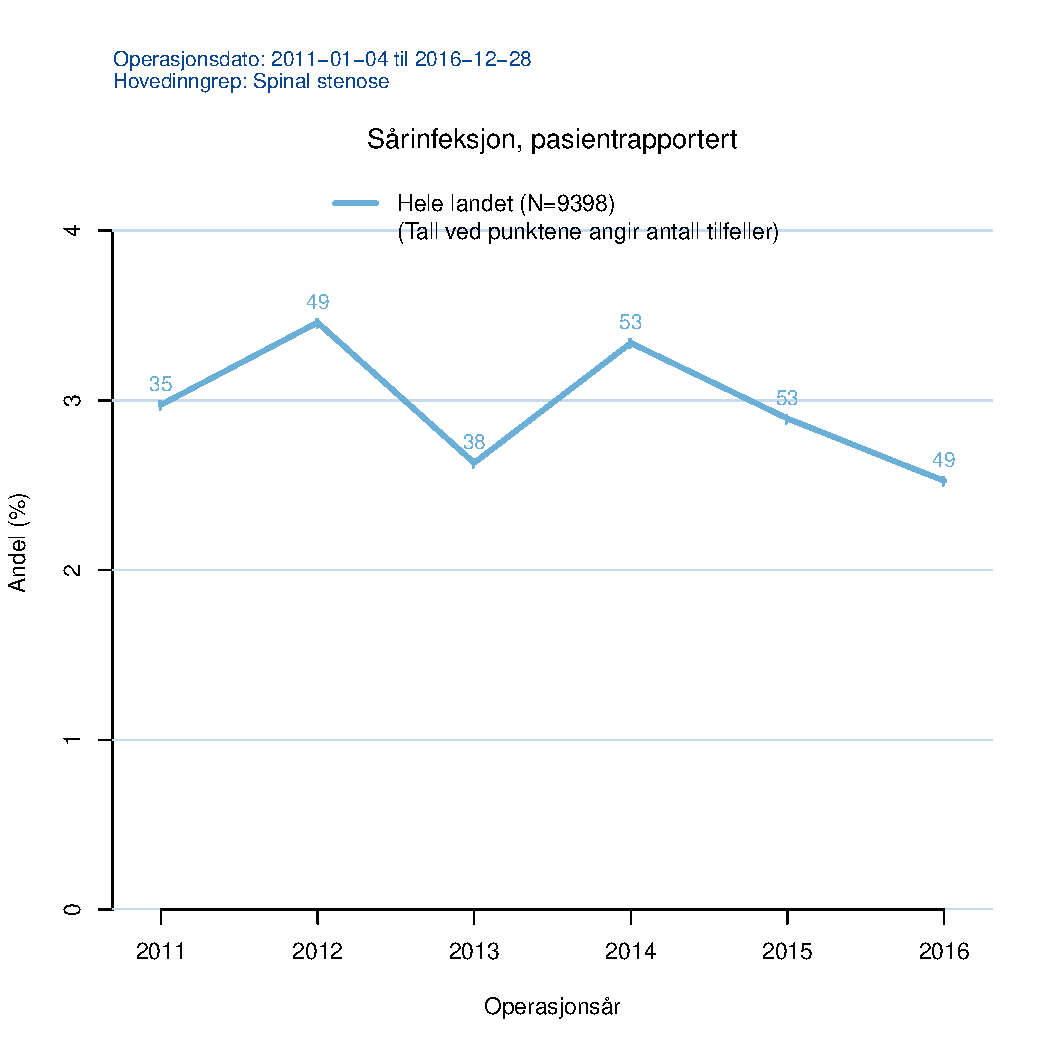
\includegraphics{Figurer/FigKpInf3MndTidSS.pdf}}
%      \caption{\label{fig:KpInfTid} Andel pasienter som rapporterer om sårinfeksjon 3 måneder etter
      %hhv. prolapskirurgi og spinal stenose, utvikling over tid.}
%\end{figure}



\begin{figure}[ht]
\scalebox{0.7}{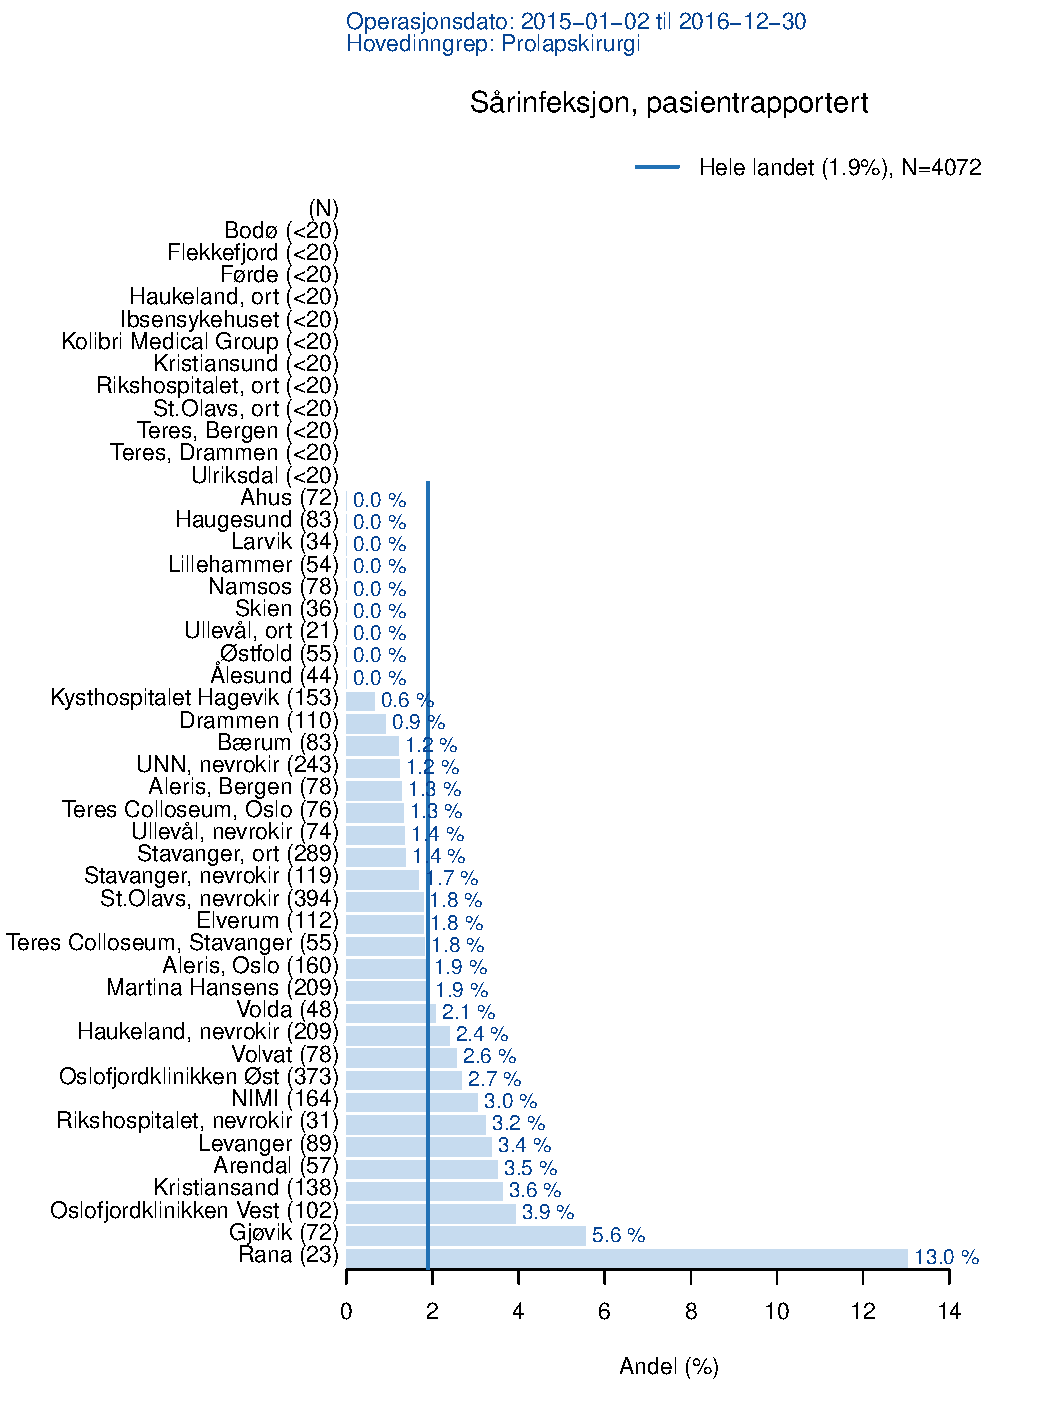
\includegraphics{Figurer/FigKpInf3MndPro.pdf}}
\caption{\label{fig:KpInfAvdPro} Andel pasienter som rapporterer om sårinfeksjon 
      (overfladisk og dyp) 3 måneder etter lumbal prolapskirurgi.}
\end{figure}

\begin{figure}[ht]
\scalebox{0.7}{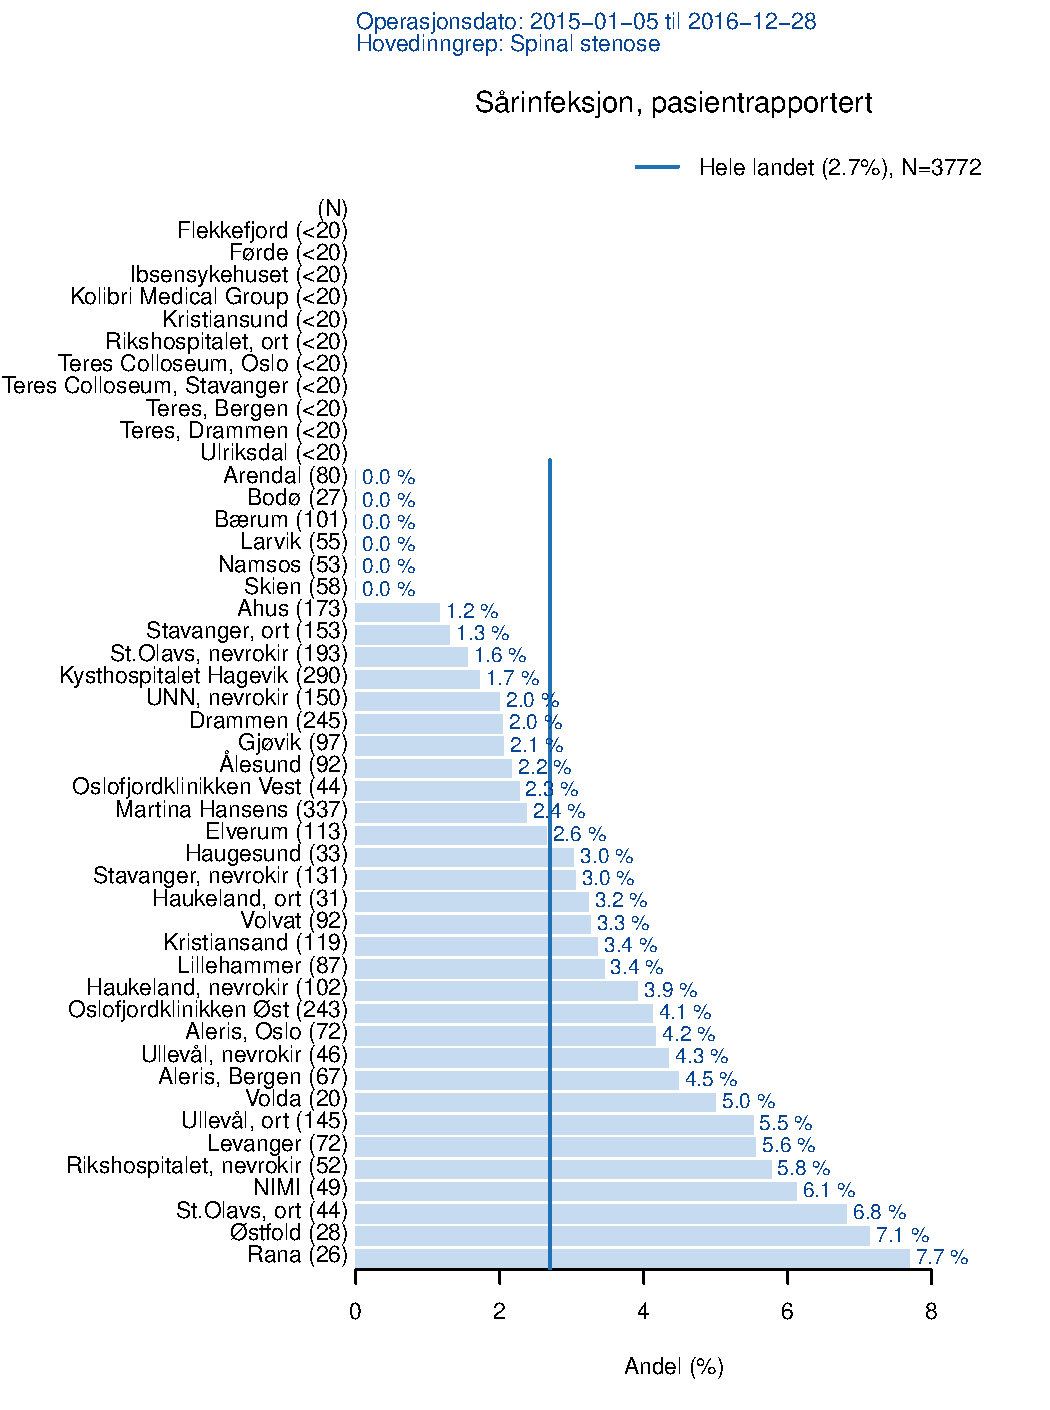
\includegraphics{Figurer/FigKpInf3MndSS.pdf}}
\caption{\label{fig:KpInfAvdSS} Andel pasienter som rapporterer om sårinfeksjon 
      (overfladisk og dyp) 3 måneder etter lumbal spinal stenose operasjon.}
\end{figure}

\clearpage

\subsubsection{Komplikasjoner (durarift)}


Durarift er oftest en ufarlig komplikasjon, men kan medføre væskelekkasje og
ubehag for pasienten, lengre liggetid og i noen tilfeller behov for reoperasjon.
Unntaksvis kan også konsekvensen være nerveskade og alvorlig infeksjon. Figurene \ref{fig:DuraPro} og \ref{fig:DuraSS} 
viser andelen som får durarift etter første gangs operasjon for henholdsvis lumbalt prolaps og spinal stenose i løpet av de to siste år.

\begin{figure}[ht]
\scalebox{0.7}{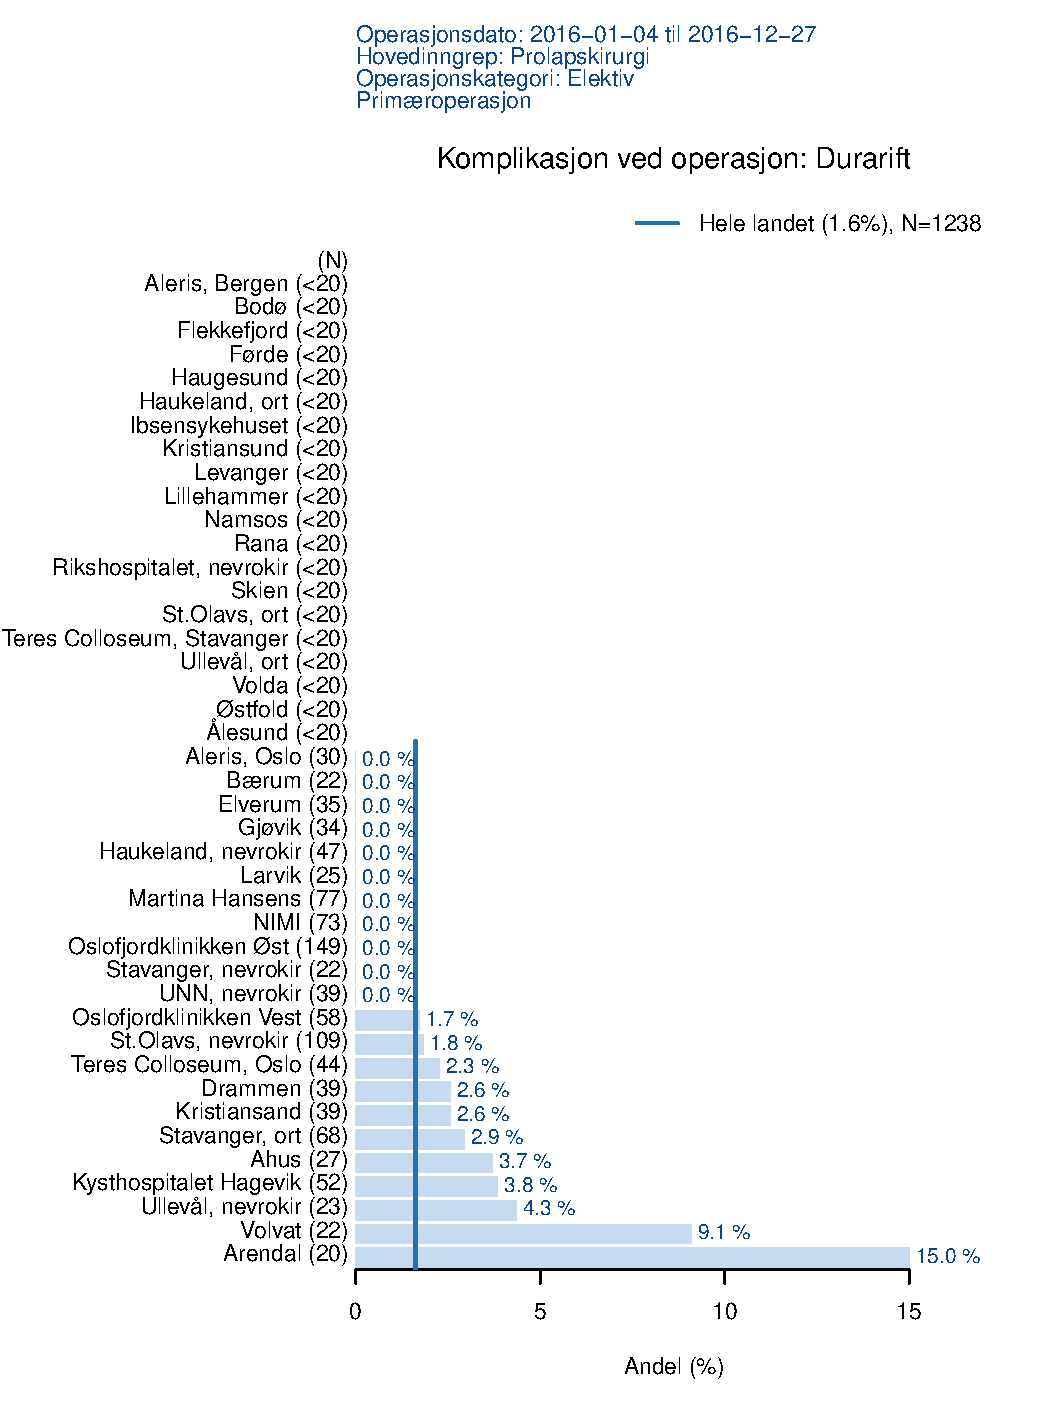
\includegraphics{Figurer/FigDuraPro.pdf}}
      \caption{\label{fig:DuraPro} Andel pasienter som fikk durarift etter kirurgi for lumbalt prolaps, 
      elektive pasienter, ikke tidligere ryggopererte.}
      \end{figure}
      
\begin{figure}[ht]
\scalebox{0.7}{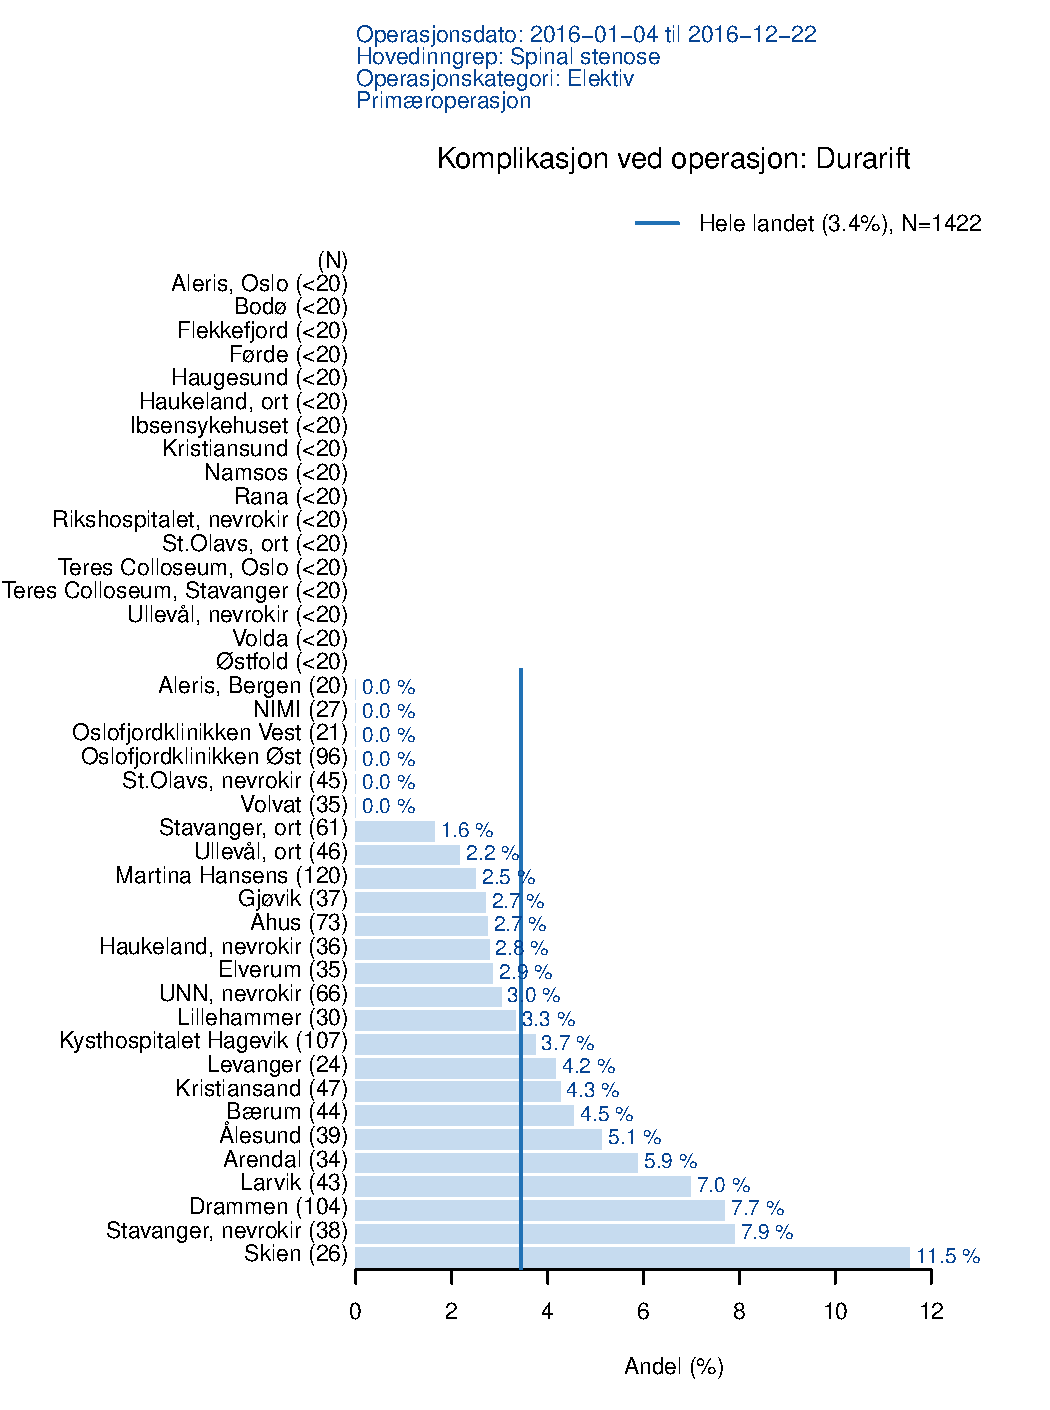
\includegraphics{Figurer/FigDuraSS.pdf}}
\caption{\label{fig:DuraSS} Andel pasienter som fikk durarift etter kirurgi for lumbal 
                  spinal stenose, elektive pasienter, ikke tidligere ryggopererte.}
\end{figure}

\clearpage



\section{Nakkekirurgi}

I Norge drives nakkekirurgi kun ved nevrokirurgiske avdelinger knyttet til de fem
universitetssykehusene i Oslo, Bergen, Trondheim, Stavanger og Tromsø, samt ved
hovedsakelig ett privat sykehus (Oslofjordklinikken, øst og vest).

Pasienter som opereres i nakken for degenerative tilstander har armsmerte med eller 
uten funksjonssvikt (radikulopati), varierende grad av nakkesmerter og noen har ryggmargspåvirkning (myelopati). 

Da  det ikke finnes nasjonale kvalitetsindikatorer for nakkekirurgi vil det bli en
viktig oppgave for NKR å utvikle slike i fremtiden. Det pågår derfor flere forskningsstudier i regi av NKR som ville kunne bidra til dette. 
Her presenteres sykehusvise data splittet på diagnose og behandling.




\subsection{Bakgrunnsdata, degenerativ nakke}


%\subsubsection{Alder, kjønn og komorbiditet}
Gjennomsnittsalder ved nakkeoperasjon var 52 år i 2017 og 84 \% ble operert med elektiv, planlagt kirurgi. Andel kvinner var  46 \%.
Andel som hadde ASA-grad over II var 9 \%. Andelen eldre over 70 år som nakkeopereres har ligget jevnt 
rundt 5 \% frem til og med 2017, men varierer noe mellom sykehus, spesielt mellom offentlige og private, 
Figur \ref{fig:NakkeAlder70Sh}.


\begin{figure}[ht]
\scalebox{0.65}{\includegraphics{Figurer/NakkeAlder70Sh.pdf}}
\caption{\label{fig:NakkeAlder70Sh} Andel nakkeopererte med alder over 70 år per sykehus}
\end{figure}

\clearpage

\subsection{Virksomhetsdata}

Som hovedregel kan ikke pasienter som opereres på grunn av ryggmargspåvirkning (myelopati) påregne bedring etter kirurgi i motsetning til de som behandles for nerverotspåvirkning (radikulopati). Hensikten med å operere de som har ryggmargsskade er snarere å forhindre forverring. Figur \ref{fig:NakkeOprIndikMyelopatiSh} viser at andelen som opereres for myelopati varierer mellom sykehusene.

\begin{figure}[ht]
\scalebox{0.7}{\includegraphics{Figurer/NakkeOprIndikMyelopatiSh.pdf}}
\caption{\label{fig:NakkeOprIndikMyelopatiSh} Andel nakkeoperete med diagnosen myelopati}
\end{figure}




\clearpage

\subsubsection{Sårdren}

Bruk av sårdren etter fremre nakkekirurgi har vært omdiskutert i litteraturen. Tidligere norske studier kan tyde på at bruk av sårdren er unødvendig, da det ikke ser ut til å redusere faren for postoperativ blødning. Figur \ref{fig:NakkeSaardrenUmFTid} viser at bruk av sårdren ved fremre nakkekirurgi er avtagende i Norge, men variasjonen mellom sykehus er stor, Figur \ref{fig:NakkeSaardrenUmFSh}.

\begin{figure}[ht]
\scalebox{0.7}{\includegraphics{Figurer/NakkeSaardrenUmFTid.pdf}}
\caption{\label{fig:NakkeSaardrenUmFTid} Andel som har hatt sårdren etter fremre nakkekirurgi i Norge per år.}
\end{figure}

\begin{figure}[ht]
\scalebox{0.7}{\includegraphics{Figurer/NakkeSaardrenUmFSh.pdf}}
\caption{\label{fig:NakkeSaardrenUmFSh} Andel som har hatt sårdren etter fremre nakkekirurgi per sykehus.}
\end{figure}

\clearpage

\subsection{Resultatmål}

Pasientene er fulgt opp med spørreskjema 3 og 12 måneder etter kirurgi.
Resultatene er ikke justert for forskjeller i pasientpopulasjonene.

%\subsubsection{Sårinfeksjon}

\subsubsection{Resultat etter fremre nakkekirurgi for nerverotssmerte og funksjonssvikt (cervical radikulopati)}




Neck Disability Index (NDI) er et godt validert mål for å vurdere bedring i smerterelatert
funksjonshemming  i dagliglivets aktiviteter samt sykdomsspesifikk livskvalitet hos 
nakkeopererte. Til å måle armsmerteintensitet før og etter operasjon brukes numerisk 
smerteskala (NRS, 0-10). Figurene nedenfor viser resultater etter fremre nakkekirurgi hos 
pasienter som har nerverotssmerte og funkssjonsvikt (radikulopati) uten tegn til 
ryggmargsskade 
(myelopati). Figur \ref{fig:NakkeNRSsmerteArmEndr12mndUmFSh} og  
\ref{fig:NakkeNDIendr12mndUmFSh} at viser at mellom 60 og 70 \% har en betydelig forbedring av 
armsmerte og funksjonssvikt (NRS og NDI reduksjon tilsvarende 30 \%  eller mer) ett år etter 
kirurgi. Det et er variasjon i resultater mellom sykehus. Over 80 \% av pasientene er fonøyde 
med behandlingen de fikk, Figur \ref{fig:NakkeFornoydBeh12mndFremSh}.  





\begin{figure}[ht]
\scalebox{0.6}{\includegraphics{Figurer/NakkeNRSsmerteArmEndr12mndUmFSh.pdf}}
\caption{\label{fig:NakkeNRSsmerteArmEndr12mndUmFSh} Andel som har fått betydelig bedring av nerverotsmerte  etter fremre nakkekirurgi, siste 2 år.}
\end{figure}

\begin{figure}[ht]
\scalebox{0.7}{\includegraphics{Figurer/NakkeNDIendr12mndUmFSh.pdf}}
\caption{\label{fig:NakkeNDIendr12mndUmFSh} Andel pasienter som har fått betydelig bedring av fysisk funksjon i dagliglivet etter fremre nakkekirurgi, siste 2 år.}
\end{figure}

\begin{figure}[ht]
\scalebox{0.7}{\includegraphics{Figurer/NakkeFornoydBeh12mndFremSh.pdf}}
\caption{\label{fig:NakkeFornoydBeh12mndFremSh} Andel pasienter som er godt fornøyd med behandlingen de fikk på sykehuset etter fremre nakkekirurgi, siste 2 år.}
\end{figure}


\clearpage

\subsubsection{Sårinfeksjon }


En av de hyppigste komplikasjonene etter nakkekirurgi er sårinfeksjon. I litteraturen er vanligvis bruk av profylaktisk antibiotikabehandling  anbefalt ved 
nakkekirurgi. Andelen som får dette har ligget stabilt og var 99,7 \% i 2017.
Ved  3 måneders etterkontroll svarer pasientene selv 
på to spørsmål  for å kartlegge dette: ''Ble du behandlet med antibiotika for overfladisk sårinfeksjon i operasjonssåret i løpet av de 4 første ukene etter operasjonen?" og 
''Har du blitt eller blir du behandlet i over 6 uker med antibiotika for dyp infeksjon i operasjonssåret?''  Forekomsten i 2017 var 
2.9 \% (totalt for bakre og fremre nakkekirurgi).  Andelen som har svart ja, ved hvert sykehus, på minst ett av disse spørsmålene er vist i Figur \ref{fig:NakkeKomplinfek3mndSh}.  

\begin{figure}[ht]
\scalebox{0.65}{\includegraphics{Figurer/NakkeKomplinfekSh.pdf}}
\caption{\label{fig:NakkeKomplinfek3mndSh} Andel pasienter som rapporterer om sårinfeksjon 3 måneder etter nakkekirurgi (fremre og bakre) i 2017. }
\end{figure}

\clearpage

\subsubsection{Komplikasjoner etter fremre nakkekirurgi}
De hyppigste komplikasjonene etter fremre nakkekirurgi er svelg og stemmevansker som følge 
av nervepåvirkning og arrdannelser. Ved etterkontroll etter 3 måneder svarer pasientene på
følgende spørsmål: ''Har du etter operasjonen vedvarende problemer med stemmen din 
(f.eks. hesthet/svak stemme)? " og " Har du etter operasjonen hatt vedvarende ubehag ved svelging av mat og drikke? "
Andelen som har svart ja på disse to spørsmålene er henholdsvis 10 \% og 16 \% i 2017, men dette  varierer mellom sykehus, Figur \ref{fig:NakkeStemme3mndSh} og \ref{fig:NakkeSvelg3mndSh}. Årsaken til disse forskjellene er uklar. 


\begin{figure}[ht]
\scalebox{0.7}{\includegraphics{Figurer/NakkeStemme3mndSh.pdf}}
\caption{\label{fig:NakkeStemme3mndSh} Andel pasienter som rapporterer stemmeproblemer 3 måneder etter fremre nakkekirurgi i 2017.}
\end{figure}

\begin{figure}[ht]
\scalebox{0.7}{\includegraphics{Figurer/NakkeSvelg3mndSh.pdf}}
\caption{\label{fig:NakkeSvelg3mndSh} Andel pasienter som rapporterer svelgproblemer 3 måneder etter fremre nakkekirurgi i 2017.}
\end{figure}





%Lena: alt nedenfor har jeg flyttet hit, skal ikke med
%\subsubsection{Varighet av smerter i rygg-/hofte og av utstrålende smerter på operasjonstidspunktet}


      
      
 

\end{document}




\chapter{Metoder for fangst av data}\label{cha:metoder}
Pasientene fyller ut spørreskjema og samtykkeerklæring som sendes ut med innkalling til ryggoperasjon. Skjema leveres ferdig utfylt ved innkomst. Alternativt deles de ut av sykepleier og sekretær ved innkomst.Legeskjema fylles ut av kirurg på operasjonsstua, enten online eller på papir, like etter at inngrepet er gjennomført, Figur \ref{fig:gangeniregistrering}. Papirskjema samles og punches inn av sekretær ved det enkelte sykehus. Ved etterkontroll sendes scannbare skjema fra NKR sitt sekretariat ved UNN, direkte til og fra pasienten, uten at behandlende sykehus er involvert. Dette forhindrer selektiv rapportering av operasjonsresultater fra sykehusene. Pasienter som ikke responderer får en påminnelse med nytt brev inkludert nytt spørreskjema. 

\begin{figure}[ht]
\includegraphics[width=\textwidth]{Figurer/gangeniregistrering.pdf}
\caption{Datafangst i NKR}
\label{fig:gangeniregistrering}
\end{figure}


\chapter{Metodisk kvalitet}\label{cha:kva}
\subsection*{Definisjoner}
\textbf{Validiteten} (gyldigheten) av den informasjonen som kommer ut av registeret er avhengig av registerets dekningsgrad, komplettheten av de innsamlede data, om opplysningene er nøyaktige/korrekte og hvor mange pasienter som responderer på spørreskjema ved etterkontroll.

\textbf{Tilslutningen} angir hvor stor andel av sykehus/avdelinger som opererer ryggpasienter som også leverer data til NKR (sykehusnivå).

\textbf{Dekningsgraden}  angir hvor stor andel av de som blir operert ved de enkelte sykehus/avdelinger som blir registrert (individnivå). 

\textbf{Kompletthet } angir mengden manglende informasjon i de spørreskjemaene som er innsamlet og registrert, dvs. ubesvarte, åpne felter («missing verdier»). 

\textbf{Nøyaktighet/korrekthet} angir om opplysningene som er gitt i spørreskjemaet avviker fra «sanne verdier» for eksempel som følge av feilrapportering, puchefeil eller feil ved skanning av skjema. 

\textbf{Responsraten } ved etterkontroll er avhengig av
at pasientene kan kontaktes/nås etter utskrivelse fra sykehus, og at de opplever det enkelt og meningsfullt å besvare spørreskjema.


\section{Antall registreringer}\label{sec:reg}
Antall operasjoner innrapportert til NKR, degenerativ rygg var 4683 i 2015 og 4841 i 2016, det vil si en økning på 3,4 \%.  
Antall operasjoner innrapportert til NKR, degenerativ nakke var 1131 i 2015 og 1033 i 2016, det vil si en nedgang på 8,6 \%. I 2016 ble det innrapportert 1219, dvs.3.0 \% færre  nakkeoperasjoner enn året før til NPR i målgruppen (alder 20 til 85 år). Dette kan indikere en ujustert dekningsgrad på 1033/1219 = 85 \%. Dekningsgraden vil imidlertid bli lavere når man tar hensyn til at den  andel av pasientene som er operert ved private sykehus er registrert i NKR, men ikke i NPR.


\section{Aktualitet}\label{sec:akt}

Data puches fortløpene inn i NKR. Ved noen sykehus kan det være en forsinklese fra hendelse (for eksempel oprasjon) til data registreres i NKR, spesielt så lenge registeret ikke er tilgjengelig gjennom EPJ. Data som er lagt i registeret er imidlertid tilgjengelig i rapportsytemet innen maximum 12 timer. Postoperative data scannes fortløpende inn i databasen. I rapportsystemet kan man få helt oppdatert informasjon om bakgrunnsvariabler, virksomhetsdata, komplikasjonsfrekvens og PROMs, samt ikke ferdigstilte skjema.
\section{Metode for beregning av dekningsgrad}\label{sec:met}

Annet hvert år utføres individbasert dekningsgradsanalyse for henholdsvis NKR degenerativ rygg og nakke med kobling mot Norsk pasientregister(NPR).
Samtykkeerklæringen til NKR dekker  sammenstilling av data. Dette er også er hjemlet i relevante bestemmelser i NPR-forskriften (§ 1 - 2b og § 3 - 7); - Saksnummer i Helsedirektoratet: 17/ 9624. Koblingsnøklene er: Pseudonymisert fødselsnummer, operasjonsdato og helseforetak.

\textbf{Dekningsgraden beregnes etter følgende formler:}

Dekningsgrad NKR : kun NKR + begge registre/kun NPR + kun NKR + begge registre

Dekningsgrad NPR : kun NPR + begge registre/ kun NKR + kun NPR + begge registre

\section{Tilslutning}\label{sec:endek}

\subsection{NKR, degenerativ rygg}
I 2016 hadde 28 av 28 helseforetak startet raportering av kirurgisk inngrep til NKR. Dette gir en tilslutning på foretaksnivå på 100 \%. 41 av 41 av sykehusavdelingene (inkludert private) rapporterer til NKR i løpet av 2016. De sykehus som ikke rapporterte til NKR  i 2015 (Sykehuset Vestfold (Tønsberg/Larvik), Førde Sjukehus og Kristiansund sjukehus) har alle startet registrering i 2016.

\subsection{NKR, degenerativ nakke}
Tilslutningen på foretaksnivå er 100 \%.  I Norge drives nakkekirurgi kun ved nevrokirurgiske avdelinger knyttet til de fem universitetssykehusene i Oslo, Bergen, Trondheim, Stavanger og Tromsø, samt ved tre privat sykehus (Oslofjorklinikken, Aleris og Volvat). 

\section{Dekningsgrad}\label{sec:obs}

\subsection{ Dekningsgrad (ledelse, systematikk)}

I henhold til oppdragsdokumentet fra Helse og omsorgsdepartementet er
sykehusene forpliktet til å rapportere til NKR. Dekningsgraden sier noe om hvor
mange operasjoner som ble rapportert i forhold til hvor mange som faktisk ble
utført ved de ulike helseforetakene. En viktig forutsetning for i det hele tatt å kunne
drive kvalitetssikring av egen virksomhet er å få kunnskap om
behandlingsresultatene gjennom NKR. Dekningsgraden er derfor en viktig
kvalitetsindikator.



\textbf{For NKR degenerativ rygg var dekningsgraden på individnivå 64,3 \%. }  1448 av 1982 inngrep kun i NKR er rapportert fra private sykehus. Disse sykehusene har kun planlagt behandling. Legges disse 1448 inngrep til NKRs dekningsgrad, øker dekningsgraden for planlagte operasjoner til 67,2 prosent for degnerativ rygg .

\textbf{For NKR degenerativ nakke var dekningsgraden tall 75 \% på indivdnivå i 2015}.Oppdaterte dekningsgradsanalyser for 2017 vil bli lagt frem i årsrapporten for 2018.



 
\textbf{Mer omfattende dekningsgradsanalyser på RHF, HF og sykehusnivå for NKR degenerativ rygg for 2016 er tilgjengelig på NKR sin hjemmeside:} \url{www.ryggregisteret.no}.


Den relativt lave dekningsgraden skyldes i første rekke manglende fokus på kvalitetssikring hos ledelsen og dårlige rutiner for
rapportering, spesielt i legegruppen. Størst er problemet for akutt kirurgi, mest i
helger, høytider og ferier.Interessen for å kvalitetssikre egen virksomhet gjennom rapportering til NKR søynes fortsatt å være størst blant private aktører og i Helse Vest og Midt-Norge innen offentlig virksomhet. 

\subsection*{Frafallsanalyser}

I årets dekningsgradsanalyse ble det gjort en frafallsanalyse på ryggopererte  som var regisitrert i NPR, men ikke i NKR. Denne viste at andel øyeblikkelig hjelp var høyere for operasjoner som kun finnes i NPR (24,9 \%) enn for operasjoner som lot seg koble mellom registrene (9,7 \%). 
Dekningsgraden til NKR var omtrent dobbelt så høy for planlagte operasjoner som for ø-hjelp, som inkluderer operasjoner utført i helger, helligdager og offentlige høytidsdager. Ryggopererte som ikke ble registrert i NKR var i gjennomsnitt tre år yngre sammenliknet de som ble registrert.






\section{Prosedyrer for intern sikring av datakvalitet}\label{sec:sik}
Alle innregistreringer av person sjekkes mot folkeregisteret. Det varsles om avvikende verdier ved punching av data, og en egen elektronisk hjelpefunksjon i databasen fungerer som rettledning. Når et skjema er fylt ut blir det varslet om manglende utfylling i en korrekturapport. Ufullstendig utfylte skjema lagres på en kladdliste som brukeren kan holde oversikt over. Egne brukermanualer er utarbeidet og kan lastes ned fra  \url{www.ryggregisteret.no}  (”Registerbeskrivelse”, ”Praktisk veileder” og ”Brukerhåndbok”). Gjennom registerets rapportsystem gis det tilbakemelding til sykehusavdelingene om manglende registreringer og sannsynlige feil. 

\section{Metode for validering av data i registeret}\label{sec:metval}
NKR benytter flere metoder for validering av data. Hensikten er i hovesak å unngå sytemstiske feil (infromasjon og seleksjons-bias). Publiering av valideringsstudiene i internasjonale fagfelle-vurderte tidsskrift er helt nødvendig for å kvalitetssikre dette arbeidet og for å gi legitimitet i fagmiljøet.Under punkt 5.8 blir det gjort næremere rede for de enkelte valideringsproskjektene i NKR:
\begin{itemize} \item {Validering av allerde innsamlede data mot eksterne kilder (data re-catch).}
\item Innhenting av data som mangler i NKR (data catch).
\item Validering av måleinstumenter (PROMs).
\item Validering av terskelverider brukt  ved sammenstilling av resultateri rapportsystemet .
\item Frafallsanalyser, se pkt. 5.5.1.

\end{itemize}

\section{Vurdering av datakvalitet}\label{sec:valdat}


\subsection{Nøyaktighet / korrekthet}

Feilregistrering etter punching av preoperative skjema: 0,3 \% 
Feilregistrering etter skanning av spørreskjema ved kontroll 3 og 12 mnd: 0,04 \% 
(Intern valideringsstudie fra april- august 2010).

NKR gjennomførte vår/sommer 2010 en valideringsstudie der data fra NKR på 470 pasienter ble sjekket mot opplysninger i sykejournalene ved en rekke sykehus.  Hovedfunnene fra denne (re-catch) studien var:

\begin{itemize}
\item Feilklassifisering av type operasjoner (inngrep) i NKR: = 3 \%
	\item Problemområder:
\begin{itemize}
		\item Komorbiditet og reoperasjoner innen 90 dager: Underrapportering
		\item ASA-klassifisering: Høy avviksprosent mellom anestesiskjema fylt
        ut før operasjon og registrerte verdier i NKR. Gjennomsnittsverdiene
        var imidlertid identiske.
\end{itemize}
\end{itemize}
\subsection{Kompletthet}

Tabell \ref{tab:kompletthet} viser kompletthet av innsamlede data i NKR degenerativ rygg.

\subsection{Responsrate ved etterkontroll}

Flere vitenskapelige artikler fra NKR publiert i internasjonale tiddsskrift viser at responsraten ved ettårskontroll er rundt 80 \% for spinal stenose opererte og rund 65-70 \% for prolapsopererte. Komplettheten av innsamlede data ved etterkontroll er høy (95 \%) og uendret fra 2011. Vi har gjennomført en (catch) studie som er publisert i 2011. Her var ”lost to follow up” 22 \%. Ved systematisk telefonintervju fant vi ingen forskjell i operasjonsresultat mellom de som returnerte og ikke returnerte (TK Solberg et al., Acta Orthop. 2011). Disse funnene ble bekreftet i en helt tilsvarende studie fra et tilsvarende  danse ryggkirurgiregister (DANEspine) i 2016 (K Höjmark et al., Eur. Spine Journal, 25: 282-6, 2016).


\subsection{Kriterier for sukksess og dårlig operasjonsresultat / ”bechmarking”}

For å kunne gjøre sammenlikninger av resultater på tvers av institusjoner har NKR gjennomført en valideringsstudie for å definere terskelverdier for å kunne karakterisere operasjonsresultat som suksessfylte (TK Solberg et al., Acta Orthop. 2013). Disse terskelverdiene innarbeides nå i NKR sitt rapportsystem. Flere nye studier ble satt igang i 2016 å definere/validere kriterier for gode og dårlige behandlingsresultat, inkludert kriterier for forverring etter kirurgi. Disse vil også bli brukt i en prediksjonsmodell som grunnlag for en riskokalkulator. Målet er å kunne beregne individuell risikoprofil slik at kalkulatoren kan brukes som felles beslutningsstøtte for pasient og kirurg. Dermed kan informasjon fra NKR om tidligere ryggoperte formidles tilbake til beslutningstakerne i forkant av operasjon, og mulige fordeler og ulemper med behandlingen blir synliggjort.


\begin{table}[ht]
\centering
\begin{tabular}{lr}
  \hline
  Variabel & Kompletthet (\%) \\
  \hline
  Alder & 99.6 \\
  Kjønn & 100.0 \\
  BMI & 99.7 \\
  Utdanning & 98.8 \\
  Sivilstatus & 99.5 \\
  Morsmål & 99.6 \\
  Røyking & 99.2 \\
  ASA-grad & 99.4 \\
  Tidligere ryggoperert? & 98.3 \\
  Bruk av smertestillende medisiner & 98.5 \\
  Bruk av antibiotika - profylakse & 98.3 \\
  Inngrep (type operasjon) & 100.0 \\
  ODI & 99.5 \\
  Ryggsmerte & 95.7 \\
  Bensmerte & 94.9 \\
  EQ-5D & 94.7 \\
  Yrkesstatus & 98.2 \\
  Helsetilstand (VAS) & 92.6 \\
  Endring i ODI (funksjon i dagliglivets aktiviteter) & 98.7 \\
  Endring i helserelatert livskvalitet (EQ-5D) & 98.3 \\
  Endring av ryggsmerte & 95.0 \\
  Endring av bensmerte & 94.9 \\
  Pasientevaluert nytte av operasjon & 99.4 \\
  Pasienttilfredshet med behandlingen & 99.0 \\
  \hline
  \end{tabular}
  \caption{Kompletthet av innsamlede data i 2016}
  \label{tab:kompletthet}
\end{table}
    


\chapter{Fagutvikling og klinisk kvalitetsforbedring}\label{cha:fag}


\section{Pasientgruppe som omfattes av registeret}
Målgruppen er pasienter som blir operert for degenerative tilstander (``aldersbetingede slitasjeforandringer'') i ryggsøylen ved alle offentlige og private sykehus. Degenerative er tilstander kan skape trange forhold for nervestrukturer på grunn av skiveprolaps, benpåleiringer, fortykkede leddbånd og feilstillinger i ryggsøylen. 
Pasientene har ofte sterke smerter, dårlig fysisk funksjon som medfører arbeidsuførhet og redusert livskvalitet. De fleste opplever en betydelig bedring av sine plager etter kirurgi.


\section{Registerets spesifikke kvalitetsindikatorer}\label{sec:regspe}

\begin{enumerate}
	\item Bench-mark kriterier for klinisk meningsfylt godt og dårlig
    operasjonsresultat bedømt med PROM (validert av NKR).
	\item Forekomst av risikofaktorer som predikerer dårlige og gode
    operasjonsresultater (virksomhetsdata og ulike
    pasientkarakteristika/bakgrunnsvariabler).
	\item Forekomst av komplikasjoner.
\end{enumerate}

Det registreres ca 350 ulike variabler i databasen til NKR. Disse kan deles i 3 hovedkategorier:

\begin{enumerate}
	\item \emph{Bakgrunnsvariabler (besvares av pasient)}: Demografiske og
    sosioøkonomiske data, samt andre kjente risikofaktorer som kan ha betydning
    for operasjonsresultatet, dvs. alder, kroppsmasse indeks (BMI), røyking,
    utdanning, co morbiditet, ASA grad, utdanning, røykevaner, sivilstatus,
    yrkesstatus med mer.  
	\item \emph{Virksomhetsdata (besvares av lege/annet helsepersonell)}: Diagnose,
    behandling, liggetid, operasjonstid, antibiotikaprofylakse, operasjonstekniske
    forhold med mer.
	\item \emph{Resultatmål (besvares av pasient)}: Her benyttes kliniske endepunkter blir i form av et sett validerte måleinstrumenter som er anbefalt
    i internasjonal litteratur; pasient rapporterte utkomme mål (patient
    reported outcome measures, PROMs). I tillegg rapporteres komplikasjoner både av kirurg og pasient.
\end{enumerate}

Nærmere beskrivelse av registerets formål, utforming, innhold, tekniske løsning og bruksområde finnes og kan lastes ned fra \url{www.ryggregisteret.no} (”Registerbeskrivelse”, ”Praktisk veileder” og ”Brukerhåndbok”)   Dette bør vi ikke ta med da de kun ser på Årsrapporten. 


\section{Pasientrapporterte resultat- og erfaringsmål (PROM og PREM)}\label{sec:pasutk}

NKR bruker PROM som indikatorer for kvalitet:
\begin{itemize}
	\item Endring av ryggspesifikk og smerterelatert funksjon i dagliglivets 
    aktiviteter og livskvalitet (Oswestry Disability Index, ODI).
	\item EQ-5D; som er et generelt livskvalitetsmål som gir mulighet til å angi 
    behandlingsresultater i kvalitetsjusterte leveår (QALYs). EQ-5D kan også brukes 
    til å sammenligne resultater på tvers av behandlinger og ulike sykdommer og til 
    kost nytte analyser.
	\item Pasientvurdert nytte av operasjon.
	\item Pasientens tilfredshet med behandlingen som ble gitt ved sykehuset (PREM).
	\item Yrkesstatus, andel av de som var sykemeldte før operasjon dom er tilbake i 
    jobb etter 3 og 12 måneder.
	\item Endring av smerte i rygg og bein (Nummerisk smerteskala).
	\item Endring av selvevaluert helsetilstand (VAS-skala).
	\item Komplikasjoner (både pasient og kirurg rapporterte).
\end{itemize}


\section{Sosiale og demografiske ulikheter i helse}\label{sec:sosdem}

I NKR registreres en rekke demografiske data (alder, kjønn, adresse (inkludert innenfor hvilket HF område pasieten bor og behandles)) , sivilstatus, utdanning, morsmål samt yrkes og trygdestatus. I tillegg registreres livsstilsfaktorer som røyking og BMI. NKR har publiert flere vitenskapelige artikler  og rapporterer om sammenhengen mellom operasjonsresultat og utdanning, røyking, fedme og fremmedspråklighet. I tillegg rapporterer NKR på forskjeller i forbruksrater av ryggkirurgi i ulike boområder (HF og RHF) 

\section{Bidrag til utvikling av nasjonale retningslinjer, nasjonale
kvalitetsindikatorer o.l.}\label{sec:retut}


I nasjonale retningslinjer for kirurgisk behandling av degenerative tilstander i ryggsøylen fra 2007 (\url{www.formi.no/images/uploads/pdf/Formi\_nett.pdf}) er anbefalingene knyttet til varighet av symptomer før prolapskirurgi. Dette rapporteres fra NKR. For øvrig finnes ingen nasjonale retningslinjer. En viktig oppgave for NKR er å utvikle flere kvalitetsindikatorer. Se forøvrig kapittel \ref{sec:brures}.

\section{Etterlevelse av nasjonale retningslinjer}\label{sec:retbru} 
Symptomvarighet under ett år anbefales ved operasjon for prolaps og er inkludert som variabel i NKR og dets rapportsystem. Forøvring finnes ingen validerte og etablerete nasjonale retningslinjer for rygg og nakkekirurgi.

\section{Identifisering av kliniske forbedringsområder}\label{sec:ide}
En Forskningsstudie fra NKR viser at antibiotika profylakse reduserer risiko for postoperativ sårinfeksjon. Bedre indikasjonsstilling og seleksjon av pasienter før kirurgi. Bedre pasientinformasjon. Raskere behandling nå indikasjon for kirurgi er stilt og ikke-kirurgisk behandling har vært forsøkt. Bedret kommunikasjon med fremmedspråklige pasienter. Reduksjon av antall multiple reoperasjoner og tilbud om alternative tiltak. Mindre invassiv/omfattende kirurgi kan gi kortere liggetid og kan dermed redusere kostnader.

\section{Tiltak for klinisk kvalitetsforbedring initiert av
registeret}\label{sec:brures}

Se punkt 6.7.  Disse resultatene har vært presentert for fagmiljøet i rapportene fra NKR, på brukermøter, kurs for spesialistkandidater innen nevrokirurgi og ortopedi i Norge og Skandinavia og i internasjonale tidsskrift.  

\section{Evaluering av tiltak for klinisk kvalitetsforbedring (endret praksis)}\label{sec:evakva}
Bruk av omfattende kirurgi ved spinal stenose går ned, også liggetid på sykehus. Bruk av synsfremmende midler ved ryggkirurgi øker. Dekningsgraden har økt betydelig ved de 4 sykehusene som har vært omfattet dekningsgradprosjektet som er gjort med støtte fra Nasjonalt servicemiljø for medisinske kvalitetsregistre. Oppdaterte dekningstall som kan evaluere effekten av dette prosjektet vil være tilgjengelig i 2018.

\section{Pasientsikkerhet}\label{sec:kom}
\textbf{En rekke variable knyttet til pasientsikkerhet registreres og rapporteres fra NKR:}

Intraoperative komplikasjoner (legerapportert):\\
Durarift, nerveskade, blødning som krever transfusjon eller reoperasjon, respiratoriske og kardiovaskulære komplikasjoner, operert feil nivå/side, anafylaksi.\\
\\Postoperative komplikasjoner (pasientrapportert):\\
Blant annet dyp og overfladisk infeksjon, DVT, lungeemboli, nevrologiske utfall oppstått etter operasjon, pneumoni, urinveisinfeksjon. Spørsmålene er hentet fra det svenske ryggkirurgiregisteret (SWEspine).\\
\\Dødsfall under sykehusopphold registreres i NKR. Dødsfall etter utskrivelse i NKR degenerativ nakke-kohorten  varsles til NKR når det er meldt til folkeregisteret.\\

 
 
\chapter{Formidling av resultater}\label{cha:dat}


\section{Resultater tilbake til deltakende fagmiljø}\label{sec:resfag}
Registerets online og interaktive rapportsystem oppdateres kontinuerlig fra databasen. Deltagende fagmiljø (autentiserte brukere) kan nå rapportsystemet (``Rapporteket'') via helseregister.no/Norsk Helsenett. Både bakgrunnsvariabler, virksomhetsdata og PROM data for hver sykehusavdeling kan evalueres og sammenliknes med et landsgjennomsnitt og de tre ``beste" avdelingene. 

Automatisk genererte samlerapporter med forhåndsdefinert fritekst viser figurer, tabeller, tallverdier og statistiske analyser basert på de data som til enhver tid er lagret databasen. Samlerapportene kan oppsummere data for ulike tidsperioder og kan splittes på kjønn, tidsperiode, type operasjon, foretaksnivå (avdeling, HF, RHF) med mer. Nye interaktive rapporter er utvikles kontinuerlig. De enkelte sykehus kan nå lage egne figurer og tabeller ved bruk av alle variablene i registeret og komponere sine egne rapporter, samt laste ned egne rådatafiler for å kunne gjøre analyser og/eller forskningsstudier. Rapporteket for NKR Degenerativ nakke ble satt i produksjon i første halvdel av 2016.


\section{Resultater til administrasjon og ledelse}\label{sec:resled}


Rapportene fra NKR sendes til de enkelte sykehusavdelingene (PDF). Årsrapportene sendes ledelsen i RHF og HF og viser resultater splittet på disse nivåene i helsetjenesten. Egne automatiserte samlerapporter kan leveres til HF eventuelt RHF med ønsket tidsintervall, dersom  ønskelig. Regionale forskjeller i operasjonsrater for nakkekirurgi i Norge ble publisert i 2015. Effektiviteten av prosjektet ``Raskere tilbake'' har vært evaluert for ryggkirurgi i 2016 gjennom et mastergradsprosjekt i helseøkonomi. NKR har levert en evalueringsrapport av spinalkirurgisk virksomhet ved henholdsvis ortopedisk og nevrokirurgisk avdeling ved Stavanger USH til Helse Stavanger HF. 

\section{Resultater til pasienter}\label{sec:respas}
Noen sykehus har valgt å offentliggjøre egne kvalitetsdata fra NKR. På UNN HF’s hjemmeside har man siden 2009 lagt ut slike data knyttet til egen virksomhet. Denne informasjonen er tilgjengelig for alle. NKR deltok på ``Ryggforeningens'' seminar ``Med ryggen mot helsevesenet'' 23. - 24. april 2016 og årsmøtet 10-11 Juni 2017. Adm. leder av denne pasientforeningen ble medlem i NKR sitt fagråd i 2016. NKR har også  presentert resultater fra NKR gjennom medlemsbladet ``Ryggstøtten'' (red. Eirik Moe). I tillegg bidrar NKR stadig oftere med aggregerte tall som brukes i erstatningssaker og tvister mellom pasient og forsikringsselskap og Norsk pasientskadeerstatning (for eksempel hyppighet av en gitt komplikasjon).

\section{Publisering av resultater på institusjonsnivå}\label{sec:off}
I årsrapportene og under den årlige presentasjonen av nye resultater fra de nasjonale medisinske kvalitetsregistrene, i regi av Nasjonalt servicemiljø for medisinske kvalitetsregistre, vises data på institusjonsnivå (antall registreringer til NKR, dekningsgrad og resultater etter prolaps, spinal stenose og nakkekirurgi (PROM)). Det presenteres også en del data på instiusjonsnivå til de deltakende fagmiljø gjennom registeres interne online rapportsystem.

\chapter{Samarbeid og forskning}\label{cha:for}
NKR sitt fagråd er et kliniker og forskernettverk. Medlemmene representerer  alle RHF-ene, både ortopediske og nevrokirurgiske spesialistforeninger, sentrale ryggforskningsmiljø i Norge samt pasientorganisasjonen ''Ryggforeningen". NKR driver allerede et utstrakt forskningssamarbeid i Norge, blant annet med Nasjonalt senter for spinale lidelser (St. Olav/NTNU), Formidlingsenheten for muskel- og skjelettlidelser (FORMI, OUS), Nasjonal samarbeidsgruppe for helseforskning (NSG; arbeidsgruppe for nasjonalt satsningsområde innen ``Muskel – og skjelettplager, skade og sykdommer'' (MUSS), NPR og NAV.  NKR er også involvert i store norske multisenter studier, bl.a. Norsk spinal stenose studie (NORDSTEN (RCT)). NKR samarbeider også med Norsk Nakke og Ryggregister (nasjonalt register for konservativ behandling ved tverrfaglige poliklinikker i spesialisthelsetjenesten), slik at de samme måleinstrumentene brukes til å evaluere overlappende pasientgrupper. 
Flere studier vedrørende indikasjonsstilling og resultat etter prolaps og spinal stenose kirurgi vil bli publisert i løpet av 2017/18. 


\section{Samarbeid med andre helse- og kvalitetsregistre}\label{sec:samfag}
Direkte kobling mot NPR for dekningsgradsanalyser er etablert.
En studie som evaluerer prosjekt ``Raskere tilbake'' i ryggkirurgipopulasjonen med kobling mot trygdregisteret i NAV er ferdigstilt. To av fagrådets medlemmer er representanter i ``The International Consortium for Health Outcomes Measurements'' (ICHOM, Harvard USA) sin ``low back pain working group''. Her jobber man med internasjonal standardisering av PROMs for bruk i kvalitetsregistre i samarbeid med registermiljø fra hele verden.  Sammenstilling av NKR data fra Norge med et lokalt kvalitetsregister i USA (Harvard, Boston) viste store forskjeller i bruk av fusjonskirurgi ved behandling av spinal stenose. Studien ble publisert i 2016. Sammenstilling av data fra Norge med kvalitetsregistre i Sverige og Danmark er gjennomført og to vitenskapelige artikler er under publisering. En studie som sammenlikner effekt («relative effectiveness» og helseøkonomi) av rygg, nakke, hofte og knekirurgi, kobler NKR data med de relevante kvalitetsregistrene (hofte og kneprotese) pågår. Resultatene forventes ferdigstilt i løpet av 2017. Data fra Helseundersøkelsen i Nord-Trøndelag (HUNT) er også koblet mot NKR i 2016 for å kunne identifisere genmarkører for kronifisering og utvikling av nevropatiske smertesyndrom. 


\section{Vitenskapelige arbeider}\label{sec:vitarb} En rekke forskningsstudier knyttet til NKR data i regi av ulike helseprofesjoner/grupper utenfor NKR er under oppstart. Ni doktorgradsprosjekter er knyttet opp mot NKR. 4 Ph.D-er og en mastergrad er fullført mens ett nytt mastergrasprosjekt er i oppstart. Resultater fra NKR har vært lagt frem for spesialistforeningene (Norsk ortopedisk, nevrokirurgisk, spinalkirurgisk forening) på kirurgisk høstmøte, på utdanningskurs for nevrokirurgiske og ortopediske spesialistkandidater, for ``Ryggforeningen'' og gjennom forskningskurs og internasjonale møter. Av 35 vitenskapelige artikler som  utgår fra NKR er 21 publisert mellom 2015 og 1. oktober 2017. I tillegg kommer registerets årsrapporter.  


\textbf{Forskningsrapporter og publiserte artikler på grunnlag av registerets data.}

1.	Jakola AS  et al. Clinical outcomes and safety assessment in elderly patients undergoing decompressive laminectomy for lumbar spinal stenosis: a prospective study. BMC.Surg. 2010

2.	Solberg TK et al. The risk of "getting worse" after lumbar microdiscectomy. Eur.Spine J. 2005

3.	Solberg TK, Olsen JA, Ingebrigtsen T et al. Health-related quality of life assessment by the EuroQol-5D can provide cost-utility data in the field of low-back surgery. Eur.Spine J 2005

4.	Solberg TK et al. Nasjonalt kvalitetsregister for ryggkirurgi. Kirurgen 2009

5.	Solberg TK, Sorlie A, Sjaavik K et al. Would loss to follow-up bias the outcome evaluation of patients operated for degenerative disorders of the lumbar spine? Acta Orthop. 2011

6.	Lønne G et al. Recovery of muscle strength after microdiscectomy for lumbar disc herniation. A prospective cohort study with 1-year follow-up. Eur.Spine J 2011

7.	Iversen T et al. Effect of caudal epidural steroid or saline injection in
chronic lumbar radiculopathy: multicentre, blinded, randomised controlled trial. BMJ 2011

8.	Sørlie A et al. Modic type I changes and recovery of back pain after lumbar microdiscetomy.  Eur.Spine J 2012

9.	Solberg TK  et al. Can we define success criteria for lumbar disc surgery?
Estimates for substantial amount of improvement in core outcome measures.  Acta Orthopaedica 2013

10.	Solberg TK .Ensuring valid and reliable data for quality control and research from a clinical registry for spine surgery Thesis. UiT, Tromsø, 2013

11.	Iversen T et al. Accuracy of physical examination for chronic radiculopathy. BMC Musculoskeletal Disorders 2013

12.	Grotle M et al. Public and private health service in Norway; a comparison of patient characteristics and surgery criteria for patients with nerve root affections due to discus herniation. Eur.Spine J 2014

13.	Lønne G et al. MRI evaluation of lumbar spinal stenosis: is a rapid visual assessment as good as area measurement? Eur.Spine J 2014

14.	Nerland US et al. Comparative effectiveness of microdecompression and laminectomy for central lumbar spinal stenosis: study protocol for an observational study. BMJ Open 2014

15.	Nerland US et al. Minimally invasive decompression versus open laminectomy for central stenosis of the lumbar spine: pragmatic comparative effectiveness study.  BMJ 2015

16.	Clement C et al. A proposed set of metrics for standardized outcome reporting in the management of low back pain. Acta Orthopaedica  2015

17.	Gulati S et al. Does daily tobacco smoking affect outcomes after microdecompression for degenerative central lumbar spinal stenosis?  Acta Neurochirurgica  2015

18.	Giannadakis C. Microsurgical decompression for central lumbar spinal stenosis: a single-center observational study. Acta Neurochirurgica  2015

19.	Nerland US et al. The risk of getting worse: Predictors of deterioration after decompressive surgery for lumbar spinal stenosis – A multicenter observational study.  World Neurosurgery 2015

20.	Giannadakis C.  Does obesity affect outcomes after decompressive surgery for lumbar spinal stenosis? – A multicenter observational registry-based study. World Neurosurgery 2015

21.	Iversen T et al. Outcome prediction in chronic unilateral lumbar radiculopathy: prospective cohort study. BMC Musculoskeletal Disorders 2015

22.	Weber C. Is there an association between radiological severity of spinal stenosis and disability, pain or surgical outcome? :  An observational multicentre study. Spine 2015

23.	Jon-André Kristiansen, Lise Balteskard et al. The use of surgery for cervical degenerative disease in Norway in the period 2008-2014: A population-based study of 6511 procedures. Acta Neurochirurgica Mar 2016

24.	Sasha Gulati, Trond Nordseth et al. Does daily tobacco smoking affect outcomes after microdecompression for degenerative central lumbar spinal stenosis? – A multicenter observational registry-based study. Acta Neurochirurgica 157 (7). May 2015

25.	Erland Hermansen, Ulla Kristina Romild et al. Does surgical technique influence clinical outcome after lumbar spinal stenosis decompression? A comparative effectiveness study from the Norwegian Registry for Spine Surgery. European Spine Journal. June 2016

26.	A Gulati, T Solberg et al. Surgery for lumbar spinal stenosis in patients with rheumatoid arthritis: A multicenter observational study. European Journal of Rheumatology 2016 

27.	Austevoll IM, Gjestad R et al. The effectiveness of decompression alone compared with additional fusion for lumbar spinal stenosis with degenerative spondylolisthesis: a pragmatic comparative non-inferiority observational study from the Norwegian Registry for Spine Surgery. European Spine Journal. July 2016

28.	Giannadakis C, Solheim O et al. Surgery for Lumbar Spinal Stenosis in Individuals Aged 80 and Older: A Multicenter Observational Study. Journal of the American Geriatrics Society. September 2016

29.	A Sørlie, S Gulati et al. Open discectomy vs microdiscectomy for lumbar disc herniation - a protocol for a pragmatic comparative effectiveness study. F1000 Research 5:2170. September 2016

30.	JH Rudolfsen. Labor market participation and “Raskere tilbake”. A study of patients suffering from lumbar disc herniation and spinal stenosis. Master thesis in economics. School of business and economics, UiT. June 2016


31. Sasha Gulati, Mattis A. Madsbu, Tore K. Solberg, Andreas Sørlie, Charalampis Giannadakis, Marius K. Skram, Øystein P. Nygaard, Asgeir S. Jakola. 8.	Lumbar microdiscectomy for sciatica in adolescents: a multicentre observational registry-based study. Acta Neurochirurgica 159(3) · January 2017

32. Mattis Madsbu, Tore K Solberg, Oyvind Salvesen, Oystein P Nygaard, Sasha Gulati. 8.	7.	Surgery for Herniated Lumbar Disk in Individuals 65 Years of Age or Older: A Multicenter Observational Study. JAMA SURGERY  February 2017

33. David A T Werner, Margreth Grotle, Sasha Gulati, [...] and Tore K Solberg.4. Criteria for failure and worsening after surgery for lumbar disc herniation: a multicenter observational study based on data from the Norwegian Registry for Spine Surgery. European Spine Journal · June 2017.

34. Samer Habiba, Oystein P Nygaard, Jens Ivar Brox, [...]and Tore K Solberg. Risk factors for surgical site infections among 1,772 patients operated on for lumbar disc herniation: a multicentre observational registry-based study. Acta Neurochirurgica 159(6) · April 2017

35. Greger Lønne, Andrew J Schoenfeld, Thomas D. Cha, [...] and Tore K Solberg. Variation in selection criteria and approaches to surgery for Lumbar Spinal Stenosis among patients treated in Boston and Norway. Clinical neurology and neurosurgery 156 · March 2017  


\onecolumn


\part{Plan for forbedringstiltak}\label{par:for}


\chapter{Forbedringstiltak}


\begin{itemize}
  \item Datafangst
    \begin{itemize}
      \item I 2016 ble papirversjonen av spørreskjema til den nye versjon 3.0 av NKR degenerativ rygg utviklet. Ved årsskiftet 2017/18 skal dataløsningen for versjon 3.0 ferdigstilles på ny plattform i OpenQreg. Man vil da tilstrebe å ta iburk arketype-variabler, spesielt knyttet til demografi og livsstil. Samtidig skal NKR flyttes over i Norsk Helsenett og et arbeid er igang for å ta ibruk datainnsamling via ''PROMS''  som er utviklet av HEMIT. Dette medfører at pasientene kan nås elektonisk (via epost, og SMS) for innsamling av opplysninger, spesielt ved etterkontroll. \item Oppgradering av NKR degenerativ nakke, som allerede ligger i OpenQreg gjennomføres i 2017 for å sikre bedre datafangst. \item Dataløsning for SMS- varsling/påminning ved etterkontroll ble etablert for NKR degenerativ rygg i 2016 og skal i drift i 2017/18. \item Et integrasjonsarbeid mellom NKR og  eletroniske pasientjournal er planlagt med oppstart 2018.
      \item Egen applikasjon for langtidsoppfølging utover ett år for selekterte grupper ryggopererte ble utviklet i 2016.
    \end{itemize}
  \item Metodisk kvalitet
    \begin{itemize}
    
      \item Med støtte fra Nasjonal servicemiljø for medisinske kvalitetsregisre gjennomførte NKR et prosjekt for å øke dekningsgraden i 2016. Fire sykehus ble besøkt og en spørreundersøkelse (Quest-Back) ble gjennomført for å kartlegge årsker til manglende innrapportering.
      \item Når ny registerplattform i OpenQreg er etablert for degnerativ rygg vil intern kvalitetssikring av data bli forbedret på linje med den oppdaterte vesjonen av degenerativ nakke som nå er i drift.
      \item I en pågående studie fra St. Olav HF blir NKR data på pasientrapportert varighet av postoperativ sykemelding etter ryggkirurg  validert mot tilsvarende data fra NAV.
      \item Et doktorgradsprosjekt knyttet til NKR data fra Helse Innlandet HF innbefatter validering av innsamlede data ved å sjekke om det er samsvar mellom data fra NKR og opplysninger i elektonisk pasientjournal. Denne studien vil også gjenta NKR sin studie fra 2010 der pasienter som ikke responderer på etterkontroll blir sporet opp og intervjuet. Dette for å se om de som ikke svarer har et annet operasjonsresultat enn de som svarer på etterkontroll. Årsaker til manglende respons vil også bli kartlagt. Et prosjekt i Helse Bergen HF validerer pasientrapportert sårinfeksjon i NKR mot opplysninger i EPJ.
      
    \end{itemize}
  \item Fagutvikling og kvalitetsforbedring av tjenesten
    \begin{itemize}
      \item Nye kvalitetsindikatorer utviklet av NKR presenteres i denne rapporten. Nye indikatorer må valideres grundig og legges frem for fagfellevurdering  (peer-review) i internasjonale tidsskrift før de eventuelt implementeres. Dette medfører et stort forskningsarbeid som pågår forløpende.  
      \item Noen nye pasientrapporterte mål som skal inn i registeret er et utvalg fra Fear Avoidance Beliefs Questionnaire (FABQ), som vil bli brukt   i prediktoranalyser.
      \item Nye demografiske variabler og livsstilsfaktorer, virksomhetsdata og sikkerhet som skal inn i versjon 3.0 av degenerativ rygg er: \begin{itemize} \item Etnisk tilhørighet, lese og skrivevansker,  bruk av snus tobakk. \item Ventetid på henholdsvis poliklinik og operasjon, pre og postopertativ liggetid. \item Bruk av trygg kirurgi prosedyre, operatørens erfaringsnivå, bruk av blodfortynnende og immunsupprimerende medisin. \end{itemize}
    
  
      \item Økt bruk av resultater til klinisk kvalitetsforbedring i hver
        enkelt institusjon, med bedre tilgang til avdelingsspesifikke rapporter. I november 2017 arrangeres praktisk kurs i minmal invassiv operasjonsteknikk (St. Olav HF) for spesialistkandidater. NKR bidrar med kurs i bedre indikasjonsstilling før kirugi basert på rapporter og publikasjoner fra NKR.
      \item Prioriterte, kliniske forbedringsområder er utvikling av risikokalkulator for bedret indikasjonsstilling for kirurgi.
    \end{itemize}
  \item Formidling av resultater: Populærvitenskaplig artikkel om behandling av spinal stenose og resultater fra NKR er under bearbeidelse. Kronikken er planlagt publiert i riksdekkende avis i løpet av 2017. Hoveresultater i årsrapport for 2016 skal legges frem for Ryggforeningens medlemsblad  Ryggstøtten. NKR vil fortsatt videreutvikle det interne rapportsystemet med fokus på avdelingsvise resultater, samt aggregering og formidling av disse til HF og RHF nivå.  

  \item Samarbeid og forskning
    \begin{itemize}
      \item Kobling av data med reseptregisteret for å kartlegge bruk av sterke smertestillende (opioider) blant ryggpasienter. Økt smarbeid med tilsvarende registre i Skandinavia og Holland med bruk av felles datasett.
         \end{itemize}
\end{itemize}




\part{Stadievurdering}


\chapter{Referanser til vurdering av stadium}


\bigskip
\bigskip

\begin{longtable}{rp{8cm}lccc}
  \caption[Vurderingspunkter for stadium \registernavn]
  {Vurderingspunkter for stadium \registernavn} \\
  \hline 	 
  Nr & Beskrivelse & Kapittel & Ja & Nei & Ikke aktuell\\ 	 
  \hline 	 
  \endfirsthead 	 
  \caption[]{forts.}\\ 	 
  \hline 	 
  Nr & Beskrivelse & Kapittel & Ja & Nei & Ikke aktuell\\
  \hline 	 
  \endhead
  \\
  \multicolumn{4}{c}{\textit{Tabellen fortsetter på neste side}} \\
  \hline
  \endfoot 	 
  \hline 	 
  \endlastfoot
   & \textbf{Stadium 2} & & \\
  1 & Er i drift og samler data fra HF i alle helseregioner
    & \ref{cha:res}, \ref{sec:endek}  & \CheckedBox
    & \Square & \Square \\
  2 & Presenterer resultater på nasjonalt nivå & \ref{cha:res} & \CheckedBox
    & \Square & \Square \\
  3 & Har en konkret plan for gjennomføring av dekningsgradsanalyser
    & \ref{sec:met} & \CheckedBox & \Square & \Square \\
  4 & Har en konkret plan for gjennomføring av analyser og løpende
      rapportering av resultater på sykehusnivå tilbake til deltakende
      enheter & \ref{sec:resfag}, \ref{sec:resled} & \CheckedBox & \Square
      & \Square \\
  5 & Har en oppdatert plan for videre utvikling av registeret
    & Del \ref{par:for} & \CheckedBox & \Square & \Square \\
    & & & & \\

   & \textbf{Stadium 3} & & \\
  6 & Kan redegjøre for registerets datakvalitet
    & \ref{sec:sik} & \CheckedBox & \Square & \Square \\
  7 & Har beregnet dekningsgrad mot uavhengig datakilde
    & \ref{sec:met}, \ref{sec:endek}, \ref{sec:obs} & \CheckedBox & \Square
      & \Square \\
  8 & Har dekningsgrad over 60 \%
    & \ref{sec:obs} & \CheckedBox & \Square & \Square \\
  9 & Registrerende enheter kan få
      utlevert egne aggregerte og nasjonale resultater
    & \ref{sec:resfag}, \ref{sec:resled}  & \CheckedBox & \Square & \Square \\
  10 & Presenterer deltakende enheters etterlevelse av de viktigste
      nasjonale retningslinjer der disse finnes
    & \ref{sec:retbru} & \CheckedBox & \Square & \Square \\
  11 & Har identifisert kliniske forbedringsområder basert på analyser fra
       registeret & \ref{sec:ide} & \CheckedBox & \Square & \Square \\
  12 & Brukes til klinisk kvalitetsforbedringsarbeid
    & \ref{sec:brures}, \ref{sec:evakva} & \CheckedBox & \Square & \Square \\
  13 & Resultater anvendes vitenskapelig & \ref{sec:vitarb} & \CheckedBox
    & \Square & \Square \\
  14 & Presenterer resultater for PROM/PREM & \ref{sec:pasutk} & \CheckedBox
    & \Square & \Square \\
  15 & Har en oppdatert plan for videre utvikling av registeret
    & Del \ref{par:for} & \CheckedBox & \Square & \Square \\
    & & & & \\

   & \textbf{Stadium 4} & & \\
  16 & Kan dokumentere registerets datakvalitet gjennom valideringsanalyser
    & \ref{sec:metval}, \ref{sec:valdat} & \CheckedBox & \Square & \Square \\
  17 & Presenterer oppdatert dekningsgradsanalyse hvert 2. år
    & \ref{sec:met}, \ref{sec:endek}, \ref{sec:obs} & \CheckedBox & \Square
      & \Square \\
  18 & Har dekningsgrad over 80\% & \ref{sec:obs} & \Square & \CheckedBox
      & \Square \\
  19 & Registrerende enheter har løpende (on-line) tilgang til oppdaterte
      egne og nasjonale resultater & \ref{sec:resfag}
      & \CheckedBox & \Square & \Square \\
  20 & Resultater fra registeret er tilpasset og tilgjengelig for pasienter
    & \ref{sec:respas} & \CheckedBox & \Square & \Square \\
  21 & Kunne dokumentere at registeret har ført til
      kvalitetsforbedring/endret klinisk praksis & \ref{sec:evakva}
      & \CheckedBox & \Square & \Square \\
  \label{tab:sta} 	 
\end{longtable}


%\listoffigures
%\listoftables

\end{document}
